\chapter{Double Higgs Boson Production Analysis}
\label{chap:DoubleHiggs}

\chapterquote{Life is really simple, but we insist on making it complicated.}%
{Confucius, 551 BC $-$ 479 BC}%: Blackwood's Magazine May 1830


Having discovered a Higgs-like particle the \LHC in 2012\cite{Aad:2012tfa,Chatrchyan:2012ufa}, it became  crucial to understand the interaction between the Higgs and other particles, and  to determine whether it is the Standard Model Higgs. A number of Higgs theories beyond the Standard Model may be tested via the double Higgs production in an electron-positron collider \cite{Kaplan:1983fs,Goldberger:2008zz}. The study of double Higgs production would prevail the  measurement of the Higgs trilinear self coupling, \gHHH, and the quartic coupling, \gWWHH. The precision for the measurement of \gHHH achievable by the Compact Linear Collider (\CLIC), is superior to that at the \LHC and the HL-LHC  \cite{Contino:2013gna}.

%The Higgs mechanism and the Higgs boson in the Standard Model have been explained in \Chapter{chap:Theory}. even with 3000$fb^{-1}$ of data

In \ee collisions, there are two main challenges with the study of the double Higgs production,  \eeToHH. Firstly, the process has a small cross section: 0.149\,fb at \rootS{1.4} and 0.588\,fb at \rootS{3}. The other challenge is that at high centre-of-mass energies, events are often boosted.  Consequently, many final-state particles are in the forward region of the detector, where the reconstruction performance is inferior to the barrel region. In addition, particles can escape detection, causing a degradation in the event reconstruction performance.


In this chapter, a full \CLICILD detector simulation study has been performed for the double Higgs production process, \eeToHH, via \WW fusion. Event generation and simulation will be discussed first. An overview of the analysis, including lepton finding and jet reconstruction, is presented, followed by an optimised multivariate analysis to distinguish signal from background processes. The optimised event selection is used to derive an estimate of the uncertainty on  \gHHH and \gWWHH measurements at \CLIC. Part  of this analysis has been published in \cite{Abramowicz:2016zbo}.
%The results of the signal selection are interpreted in the context of the Higgs self coupling.

\section{Analysis strategy overview}

The study of double Higgs production via \WW fusion can probe the Higgs trilinear self coupling, \gHHH, and quartic coupling, \gWWHH. Leading-order Feynman diagrams for double Higgs production via \WW fusion are shown in \Figure{fig:doubleHiggsFeynman}. The diagram shown in  \Figure{fig:doubleHiggsFeynman1} contains the triple Higgs vertex, which is sensitive to the Higgs trilinear self coupling \gHHH. The diagram in the \Figure{fig:doubleHiggsFeynman2} is sensitive to the quartic coupling \gWWHH. Figures \ref{fig:doubleHiggsFeynman3} and \ref{fig:doubleHiggsFeynman4} show the Feynman diagrams for irreducible background processes in the study of \gHHH and \gWWHH.


\begin{figure}[!htbp]
  \begin{subfigure}[b]{0.22\textwidth}
    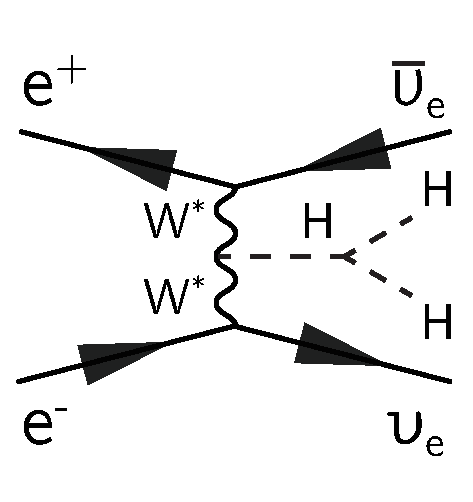
\includegraphics[width=\textwidth]{{{doubleHiggs/Feynman/1}}}
    \caption{}
    \label{fig:doubleHiggsFeynman1}
  \end{subfigure}
  \begin{subfigure}[b]{0.22\textwidth}
    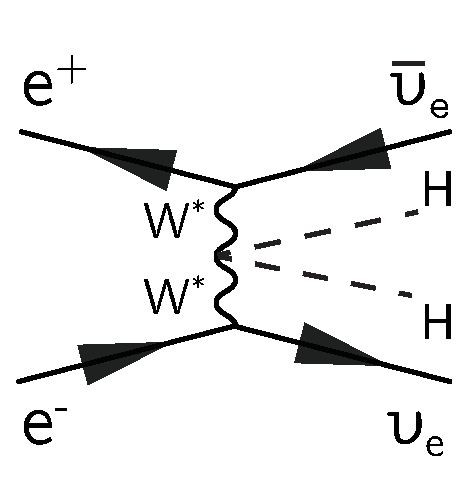
\includegraphics[width=\textwidth]{{{doubleHiggs/Feynman/2}}}
    \caption{}
    \label{fig:doubleHiggsFeynman2}
  \end{subfigure}
  \begin{subfigure}[b]{0.22\textwidth}
    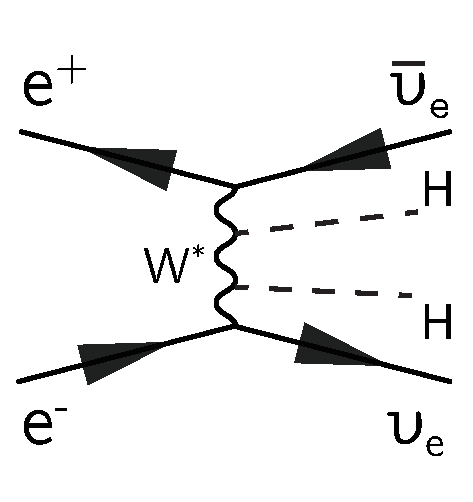
\includegraphics[width=\textwidth]{{{doubleHiggs/Feynman/3}}}
    \caption{}
    \label{fig:doubleHiggsFeynman3}
  \end{subfigure}
  \begin{subfigure}[b]{0.22\textwidth}
    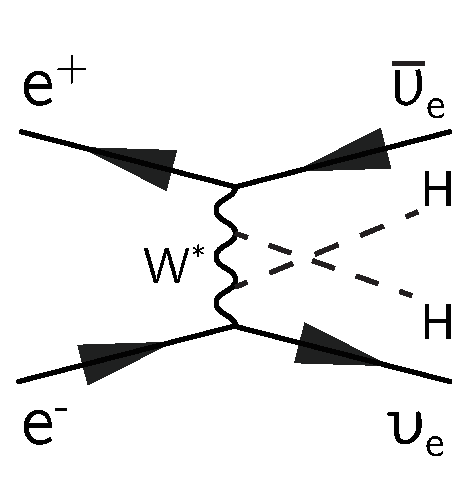
\includegraphics[width=\textwidth]{{{doubleHiggs/Feynman/4}}}
    \caption{}
    \label{fig:doubleHiggsFeynman4}
  \end{subfigure}
\caption
   {The main Feynman diagrams for the leading-order \eeToHH processes at \CLIC.}
   \label{fig:doubleHiggsFeynman}
\end{figure}

Double Higgs production can   also  be procduced via {\HepProcess{ \Pep \Pem \to \PZ \PHiggs \PHiggs}\xspace}, where the \PZ decays to \HepProcess{\Pnu \APnu}. The \HepProcess{\PZ \PHiggs \PHiggs} process has been studied in  \ee collisions at \rootSGeV{500} \cite{Baer:2013cma}. However, for the \CLIC energies of \rootS{1.4} and 3\,TeV, its contribution to the \HepProcess{\PHiggs \PHiggs \Pnu \APnu} final state is small compared to that of the \WW fusion, and it can be neglected.

%The cross section of {\HepProcess{ \Pem \Pep \to \PZ \PHiggs \PHiggs}\xspace} is one order of magnitude smaller than \eeToHH via the \WW fusion,  shown in \Figure{fig:theoryHiggsCrossSection},. Therefore, the effect of {\HepProcess{ \Pem \Pep \to \PZ \PHiggs \PHiggs}\xspace} present in \eeToHH channel at \rootS{1.4} and 3\,TeV is negligible.


%However, {\HepProcess{ \Pem \Pep \to \PZ \PHiggs \PHiggs}\xspace} can be easily identified via the recoil mass. Hence {\HepProcess{ \Pem \Pep \to \PZ \PHiggs \PHiggs}\xspace} is not considered in this studied.

The two Higgs in the  \eeToHH decay to a range of particles. Hence  double Higgs production has several distinct final-state topologies. The sub-channel with the largest cross section, \eeToHHbbbb, has been studied by  collaborators at \CERN. In this chapter, the \eeToHHbbWW sub-channel  is investigated. Firstly, the \eeToHHbbWW sub-channel is studied for fully hadronic decays of the \WW; fully hadronic \WW decays have the largest branching fraction and the lack of neutrinos in the final states allows each \PW to be reconstructed. The semi-leptonic final state of the \WW system in \eeToHHbbWW is also studied. Here the presence of the neutrino in the final state makes it  difficult to reconstruct the two Higgs bosons.

 %hadronic decay of the \WW in the \eeToHHbbWW channel is studied, because the hadronic decay has the largest cross section  in the \eeToHHbbWW channel . The hadronic decay sub-channel  does not have   neutrinos in the final state, which allows each \PW to be reconstructed. The semi-leptonic final state of the \WW system in the \eeToHHbbWW is also studied. The presence of the neutrino in the final state makes it  difficult to reconstruct the two Higgs bosons, as some momenta of one Higgs boson is carried by the neutrino. %This channel is discussed briefly and its analysis strategy is adapted from the hadronic decay analysis.
%The double Higgs production, \eeToHH, is divided into two sub-channel: \eeToHHbbWW and \eeToHHbbbb to target the specific kinematic properties if each final state, which provides cross-validation between two sub-channels and an improvement in signal selection when combined.


%However, hadronic decay final state of the \eeToHHbbWW has a very low cross section. The signal selection is challenging and aggressive background rejection methods are deployed.
%The analysis of the \eeToHHbbbb  sub-channel has been studied independently by collaborators. In this thesis, two analyses are combined for the final couplings extractions.
%The    is studied independently by collaborators. However, there is collaboration between the two studies. The two analyses are combined on the final couplings extractions.

%Combining with the low cross section, results for these two final states are not reported. The analysis can be easily (and have been) adapted for the semi-leptonic and leptonic final states.

The process, \eeToHHbbWWHadFull, results in a six quark final state with missing momentum. The high number of quarks requires an efficient jet reconstruction and a jet pairing algorithm to select the signal events. The two \Pbottom quarks in the final state can be identified statistically with \Pbottom jet tagging. %Since the final state does not contain leptons, event-level lepton finding - typically for energetic isolated leptons -  would improve the signal selection efficiency.

The chapter is organised as follows. Firstly, suitable signal and background processes are identified. Events with isolated high-energy leptons are discarded.  Vertex information is used to identify \Pbottom quark jets, in return to help to select signal events. The particles are clustered into jets and the jets are used as inputs for pre-selection and multivariate analysis.

The event reconstruction was first performed for \rootS{1.4} and then \rootS{3}, using the Marlin framework and reconstruction package in \ilcsoft v01-16. More details on the reconstruction software can be found in \Chapter{chap:Reconstruction}.

% The \eeToHHbbWW hadronic decay will be presented first, followed by the semi-leptonic sub-channel analysis.


\section{Monte Carlo sample generation}

A full list of generated samples with their cross sections can be found in \Table{tab:doubleHiggsMCSamples}. All samples were generated with the \CLICILD detector model.
% TODO
% Understand beamsstrahlung and EPA
%For this simulation study, the first step is to generate Monte Carlo samples. A full list of generated samples with their cross sections can be found in \Table{tab:doubleHiggsMCSamples}. The software for Monte Carlo sample generation used  is described in \Section{sec:pandoraMC}.

At high centre-of-mass energies, in addition to considering electron-electron interactions, electron-photon and photon-photon interactions are important as their interactions become significant. These photons are produced due to the high electric field generated by the colliding beams. Processes involving real photons from beamsstrahlung (BS) and ``quasi-real'' photons are generated separately. For the ``quasi-real'' photon initiated processes, the Equivalent Photon Approximation (EPA) has been used \cite{lyth:jpa00215525}.

%Background samples considered in this analysis are listed in Table \ref{tab:doubleHiggsMCSamples}. The signal channel is \eeToHHbbWWFull where both \PW 's decay hadronically.
%W's decay hadronically? Does this make sense from a physics point of view?
%The analysis is performed with \CLICILD detector concept at \rootS{1.4} and 3\,TeV, and the semi-leptonic channel. Unless specified, the

Background processes with multiple quarks and missing momentum in the final states are challenging to reject, as the topologies are similar to that of the signal events. Two example background processes are \eeTo{ \Pquark \Pquark \Pquark \Pquark \Pnu \APnu} and \HepProcess{\Pepm\Pphoton \to \Pnu \Pquark \Pquark \Pquark \Pquark}. For the same reason, single Higgs boson production, such as \eeTo{\Pquark \Pquark \PHiggs \Pnu \APnu}, has a similar final state to the signal events and is also difficult to reject.

Some processes are not considered in this analysis because they either have very different event topologies to the signal, or they have very small cross sections. For example,  \HepProcess{\Egamma   \to \Pquark \Pquark \PHiggs \Plepton} is neglected  as the cross section is very small, even at \rootS{3}.

%For example, six-quark final states were not simulated due to constraints of the simulating software.
The background processes are generated according to the final states fermions and usually correspond to the contributions from multiple Feynman diagrams. These diagrams are already accounted for in the generated samples for explicit Higgs production.   Therefore, to separate Higgs production from other processes, all background processes are generated with a Higgs boson mass of 14\,TeV to ensure a negligible Higgs contribution. Processes involving Higgs production are simulated with a Higgs boson mass of 126\,GeV.

%. The final states of background processes could also happen via Higgs production, which would result in double counting of Higgs events with signal sample.

The cross section of the signal, \eeToHHbbWW, is scaled according to values listed in \cite{Dittmaier:2012vm}, as the values are more updated than the  default Higgs branching ratios in the generator software.

 %the default Higgs branching ratios in the generator software are less accurate than the values listed in \cite{Dittmaier:2012vm}.

%Multi-quark final state background samples could, in principle, contain higgs production. Therefore, they are generated with a Higgs mass of 14\,TeV. This will

% ATTN need to rewrite
The simulation and reconstruction chain is described in \Chapter{chap:Reconstruction}. For some background processes, events are generated requiring that the invariant mass of the total momenta of all quarks is above 50\,GeV or 120\,GeV.This restricts the event generation to the region of phase space that could be populated by the signal processes.

% because the invariant masses of the visible momenta of signal events are mostly above 150\,GeV.

%   For electron-photon interaction with $\Pquark\Pquark\Pquark\Pquark\Pnu$ final state at \rootS(1.4), events are simulated requiring invariant mass of quarks above 120\,GeV.

% These generator level cuts requires  limits are necessary to generate a large amount of background samples in a feasible timeframe, without losing significant signal samples.

Finally, the beam induced background, \ggHad, is simulated and overlayed on all events. Details can be found in \Section{sec:pandoraggHad}.
% according to the integration time of each subdetector

\begin{table}[!htbp]\centering
% TODO fix lumi correction for e gamma, gamma e
% TODO change some of sample cross section for  electron-photon interaction with four quarks and a neutrino final state

%{
\begin{tabular}{lr}
\hline \hline
Process \rootS{1.4} &  $\sigma$ / fb   \\
\hline
\eeToHH & 0.149 \\
\hline
\eeToHHbbWWFull,hadronic & 0.018  \\
\eeToHHbbbbFull & 0.047 \\
\eeToHHotherFull & 0.085 \\
\hline
\eeTo{\qlight \qlight \PHiggs \Pnu \APnu}  & 0.86 \\
\eeTo{\Pcharm \APcharm \PHiggs \Pnu \APnu}  & 0.36 \\
\eeTo{\Pbottom \APbottom \PHiggs \Pnu \APnu}  & 0.31 \\

\eeTo{ \Pquark \Pquark \Pquark \Pquark}   &   1245.1\\
\eeTo{ \Pquark \Pquark \Pquark \Pquark \Plepton \Plepton}& 62.1* \\
\eeTo{ \Pquark \Pquark \Pquark \Pquark \Plepton \Pnu}& 110.4*\\
\eeTo{ \Pquark \Pquark \Pquark \Pquark \Pnu \APnu} & 23.2* \\

\eeTo{ \Pquark \Pquark} &  4009.5\\
\eeTo{ \Pquark \Pquark \Plepton \Pnu} &  4309.7\\
\eeTo{ \Pquark \Pquark \Pl \Pl} &  2725.8 \\
\eeTo{ \Pquark \Pquark \Pnu \Pnu} & 787.7  \\
\hline
\egamma{\Pepm}{\Pphoton}{\BS}{\Pepm \Pquark \Pquark \Pquark \Pquark} & 2317  \\
%\egamma{\Pem}{\Pphoton}{BS}{\Pem \Pquark \Pquark \Pquark \Pquark} & 1160.7  \\
%\egamma{\Pep}{\Pphoton}{BS}{\Pep \Pquark \Pquark \Pquark \Pquark} & 1156.3 \\
\egamma{\Pepm}{\Pphoton}{\EPA}{\Pepm \Pquark \Pquark \Pquark \Pquark} & 574 \\
%\egamma{\Pem}{\Pphoton}{EPA}{\Pem \Pquark \Pquark \Pquark \Pquark} & 287.1 \\
%\egamma{\Pep}{\Pphoton}{EPA}{\Pep \Pquark \Pquark \Pquark \Pquark}  & 286.9 \\
\egamma{\Pepm}{\Pphoton}{\BS}{\Pnu \Pquark \Pquark \Pquark \Pquark}& 159.1\myDagger \\
%\egamma{\Pem}{\Pphoton}{BS}{\Pnu \Pquark \Pquark \Pquark \Pquark}& 79.8\myDagger \\
%\egamma{\Pep}{\Pphoton}{BS}{\APnu \Pquark \Pquark \Pquark \Pquark}& 79.3\myDagger \\
\egamma{\Pepm}{\Pphoton}{\EPA}{\Pnu \Pquark \Pquark \Pquark \Pquark}& 34.7\myDagger  \\
%\egamma{\Pem}{\Pphoton}{EPA}{\Pnu \Pquark \Pquark \Pquark \Pquark}& 17.4\myDagger  \\
%\egamma{\Pep}{\Pphoton}{EPA}{\APnu \Pquark \Pquark \Pquark \Pquark}& 17.3\myDagger  \\
\egamma{\Pepm}{\Pphoton}{\BS}{\Pquark \Pquark \PHiggs \Pnu} & 31.5* \\
%\egamma{\Pem}{\Pphoton}{BS}{\Pquark \Pquark \PHiggs \Pnu} & 15.8* \\
%\egamma{\Pep}{\Pphoton}{BS}{\Pquark \Pquark \PHiggs \Pnu} & 15.7* \\
\egamma{\Pepm}{\Pphoton}{\EPA}{\Pquark \Pquark \PHiggs \Pnu} & 6.78* \\
%\egamma{\Pem}{\Pphoton}{EPA}{\Pquark \Pquark \PHiggs \Pnu} & 3.39* \\
%\egamma{\Pep}{\Pphoton}{EPA}{\Pquark \Pquark \PHiggs \Pnu} & 3.39*   \\
\hline
\gammagamma{\Pphoton}{\BS}{\Pphoton}{\BS}{ \Pquark \Pquark \Pquark \Pquark}& 21406.2*  \\
\gammagamma{\Pphoton}{\BS}{\Pphoton}{\EPA}{ \Pquark \Pquark \Pquark \Pquark}& 4018.7* \\
\gammagamma{\Pphoton}{\EPA}{\Pphoton}{\BS}{ \Pquark \Pquark \Pquark \Pquark}& 4034.8* \\
\gammagamma{\Pphoton}{\EPA}{\Pphoton}{\EPA}{ \Pquark \Pquark \Pquark \Pquark}& 753.0* \\
\hline \hline
\end{tabular}

\caption[Signal and background samples with the corresponding cross sections at \rootS{1.4}.]
{List of signal and background samples used in the double Higgs analysis with the corresponding cross sections at \rootS{1.4}. \Pquark can be \Pup, \Pdown, \Pstrange, \Pbottom or \Ptop. Unless specified, \Pquark, \Plepton and \Pnu represent either particles or the corresponding anti-particles. \Pphoton(BS) represents a real photon from beamstrahlung (BS). \Pphoton(EPA) represents a ``quasi-real'' photon, simulated with the Equivalent Photon Approximation. For processes labeled with * and $\myDagger$, events are generated with the invariant mass of the total momenta of all quarks above 50 and 120\,GeV, respectively.}
\label{tab:doubleHiggsMCSamples}
\end{table}
%Simulated \PW has invariant mass of 80.385\,GeV.

\section{Lepton identification}
\label{sec:doubleHiggsLepton}

For the signal process, \eeToHHbbWWHad, there is no primary lepton in the final state, whilst many background  processes, such as \HepProcess{\Pquark \Pquark \Pquark \Pquark \Plepton \Pnu}, contain primary leptons in final states. Hence, efficiently rejecting events with primary leptons is an important step in the event selection. Primary leptons deposit energies in the tracking detector. The impact parameter to the interaction point of the fitted track of the primary lepton is typically small. At the same time, the primary leptons often have energies above 10\,GeV and are  isolated from other particles. High-energy electrons and muons are stable enough to deposit energies in the calorimeters. However,  tau leptons are short lived with a typical decay lifetime of 290\,fs\cite{Abreu:1991jn}. They decay before reaching the vertex detector. Therefore, only the decay products of the tau leptons can be reconstructed.


%New processors have been developed and existing processors have been optimised for signal selection and background rejection.
%The reconstruction is done via Marlin in \ilcsoft v01-16. The latest functioning flavour tagging processor exist in \ilcsoft v01-16. Thus newer versions of  \ilcsoft can not be used in this analysis.



\subsection{Electron and muon identification}
\label{sec:doubleHiggsLeptonID}

Two approaches to electron and muon identification were utilised, which are described below. The performance is summarised in \Table{tab:doubleHiggsIsoLepPerformance}.

%Two Marlin reconstruction for processors for light lepton(\Pe, \Pmu) tagging are used and optimised. As it is important to identify primary light leptons to help to select signal events, two additional light lepton tagging processors are developed and optimised.

 %described followed by their performances. As the signal is very rare comparing to the background, it is necessary to develop high performance isolated lepton finder to veto events with leptons and improve the signal selection efficiency. An existing lepton finder is optimised in \Section{sec:doubleHiggsIsolatedLeptonFinder} and a separate lepton finder is developed by the author in \Section{sec:doubleHiggsBonoLeptonFinder}.

\subsubsection{\IsolatedLeptonFinderProcessor}
\label{sec:doubleHiggsIsolatedLeptonFinder}
An optimised version of the existing  \IsolatedLeptonFinderProcessor reconstruction package is used. This algorithm identifies high energy electrons and muons that are isolated from other particles. The algorithm parameters were optimised by the collaborator using the \eeToHHbbbb as the signal process and the \eeTo{ \Pquark \Pquark \Pquark \Pquark \Plepton \Pnu} as the background process, as the background processes are the same for this analysis with \eeToHHbbWW process.

%, which is a multi-quark final state containing a primary lepton.

%Electron induced electromagnetic showers are mostly contained in the \ECAL. The primary electrons and muons from the electron-positron interaction leaves primary tracks in the tracking detector, which start typically less than 0.05\,mm from the interaction point. The isolation criteria requires the lepton to be spatially separated from other high energy particles.

Optimal values of the parameters of the \IsolatedLeptonFinderProcessor are listed in \Table{tab:doubleHiggsIsolatedLeptonFinder}: $E$ is the energy of the lepton; $E_{\ECAL}$ is the energy of the lepton deposited in the \ECAL; $E_{cone}$ is the total energy within a cone of an opening angle of $\cos^{-1}(0.995)$ around the lepton; and the impact parameters, $d_0$, $z_0$, and $r_0$ are the closest Euclidean distance of the fitted track of the primary lepton to the interaction point  in $x$-$y$ plane, in $z$ direction, and in $x$-$y$-$z$ three dimensional space, respectively.



%in mm of the lepton track starting point to the interaction point

\begin{table}[!htbp]
\begin{tabular}{lr}
\hline
\hline
\IsolatedLeptonFinderProcessor  & Selection \\
\hline
High Energy &  $E > 15$\,GeV  \\
\Pepm ID & $\frac{E_{\ECAL}}{E} > 0.9$ \\
\Pmupm ID &  $ 0.25> \frac{E_{ECAL}}{E} > 0.05$\\
Primary Track  & $d_0$ < 0.02\,mm;\, $z_0$ < 0.03\,mm;\, $r_0$ < 0.04\,mm \\
Isolation & $E_{cone}^2 \leqslant 5.7\,\uprightMath{GeV} \times E - 50\,\uprightMath{GeV^{2}}$ \\
\hline
\hline

\end{tabular}
\caption
{Optimised parameters of the \IsolatedLeptonFinderProcessor processor.}
\label{tab:doubleHiggsIsolatedLeptonFinder}
\end{table}

\subsubsection{\BonoLeptonFinder}
\label{sec:doubleHiggsBonoLeptonFinder}

A complimentary electron finder, \BonoLeptonFinder, was developed to further identify isolated electrons and muons. Compared to the \IsolatedLeptonFinderProcessor, the main difference is that the \BonoLeptonFinder utilises particle ID information provided by the \pandora reconstruction to identify leptons.

%\IsolatedLeptonFinderProcessor has strict criterion to find high-energy isolated leptons to avoid mistakes. However, since the signal cross section is low in this analysis, it would be beneficial to reject more events with leptons identified to improve the signal to background ratio. Hence another isolated lepton finder is developed. The main feature of the \BonoLeptonFinder is that it utilises calorimetric information provided by \pandora.

\TABLE{tab:doubleHiggsBonoLeptonFinder} lists the  selection cuts for \BonoLeptonFinder. The variables in the \IsolatedLeptonFinderProcessor and the \BonoLeptonFinder are defined in the same way. In addition: \pT is the transverse momentum; $E_{cone1}$ and $E_{cone2}$ are the total energy of PFOs within a cone around the lepton  of an opening angle of $\cos^{-1}(0.995)$ and $\cos^{-1}(0.99)$ respectively.


The algorithm uses two sets of cuts to identify isolated leptons. If a PFO passes either set of cuts, it will be identified by the processor. The first set of cuts uses the particle ID information from \pandora, demanding a \pandora electron or muon with high energy above 10\,GeV and $r_0$ < 0.015\,mm. Afterwards, the lepton should either have $\pT > 40$\,GeV, or $E \geqslant 23\,\uprightMath{GeV^{\frac{1}{2}}} \times \sqrt{E_{cone1}} + 5\,\uprightMath{GeV}$. \FIGURE{fig:doubleHiggsBonoIsoLepE1HighPTSgl} and \ref{fig:doubleHiggsBonoIsoLepE1HighPTBkg} show the distributions of the \pT of identified electrons after  $E$  and $r_0$ cuts, for  \eeToHHbbWWHad signal process and \eeTo{ \Pquark \Pquark \Pquark \Pquark \Plepton \Pnu}  background process respectively. A cut of $\pT > 40$\,GeV preserves most signal events. \FIGURE{fig:doubleHiggsBonoIsoLepE1LowPTSgl} and \ref{fig:doubleHiggsBonoIsoLepE1LowPTBkg} show the distributions of $23\,\uprightMath{GeV^{\frac{1}{2}}} \times \sqrt{E_{cone1}} + 5\,\uprightMath{GeV}$ as a function of $E$ of identified electrons after  $E$  and $r_0$ cuts, for  \eeToHHbbWWHad signal process and \eeTo{ \Pquark \Pquark \Pquark \Pquark \Plepton \Pnu}  background process respectively. A cut along the two-dimensional histogram would discard background events and leave signal events intact.

%which is

The second set of cuts is similar to the first set of cuts. Apart of the differences in the values of the cuts, lepton ID in the second set of  cuts is determined using the fraction of the energy deposited in the \ECAL as a function of the total energy,  $\frac{E_{\ECAL}}{E}$: if $\frac{E_{\ECAL}}{E}$  > 0.95 then the PFO is an electron; and if  $0.2 > \frac{E_{\ECAL}}{E} > 0.05$  then the PFO is a muon.

% uses \ECAL energy fraction, which for a PFO is the energy deposited in the \ECAL divided by the total energy, to determine the lepton ID. The rest of the cuts are very similar to the first cuts. The second set cuts have stricter isolation criterion to reduce fake rate.
%Not sure the last sentence above makes sense




\begin{table}[!htbp]
\begin{tabular}{lr}
\hline
\hline
\BonoLeptonFinder  & Selection \\
\hline
High Energy &  $E > 10$\,GeV  \\
\Pepm ID & \pandora reconstructed;\, $\frac{E_{\ECAL}}{E} > 0.95$ \\
\Pmupm ID &  \pandora reconstructed\\
Primary Track & $r_0 < 0.015$\,mm \\
\hspace{3mm} a) High Transverse Momentum, or  &  $\pT > 40$\,GeV  \\
\hspace{3mm} b) Isolation & $E \geqslant 23\,\uprightMath{GeV^{\frac{1}{2}}} \times \sqrt{E_{cone1}} + 5\,\uprightMath{GeV}$ \\
\hline
High Energy  &  $E > 10$\,GeV  \\
\Pepm ID & $\frac{E_{\ECAL}}{E} > 0.95$ \\
\Pmupm ID & $0.2 > \frac{E_{\ECAL}}{E} > 0.05$ \\
Primary Track & $r_0 < 0.5$\,mm \\
\hspace{3mm} a) High Transverse Momentum, or &  $\pT > 40$\,GeV  \\
\hspace{3mm} b) Isolation & $ E \geqslant 28\,\uprightMath{GeV^{\frac{1}{2}}} \times \sqrt{E_{cone2}} + 30\,\uprightMath{GeV}$ \\
\hline
\hline

\end{tabular}
\caption[Optimised parameters  of \BonoLeptonFinder.]
{Optimised parameters  of  the \BonoLeptonFinder processor. A PFO needs to pass either set of cuts to be identified as a isolated electron or muon. Within a set of cuts, the PFO needs to satisfy either condition a) or b).}
\label{tab:doubleHiggsBonoLeptonFinder}
\end{table}



\begin{figure}[!htbp]
  \begin{subfigure}[b]{0.45\textwidth}
    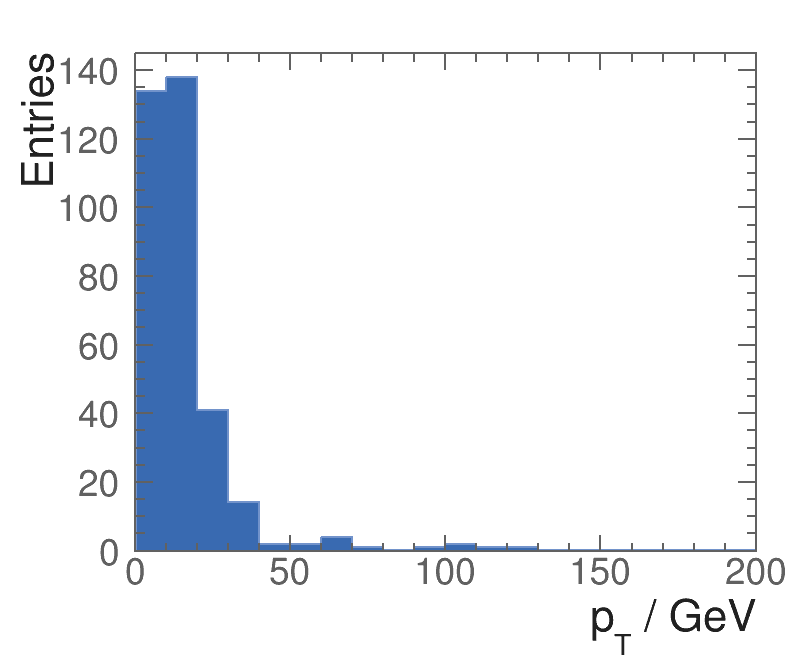
\includegraphics[width=\textwidth]{{{doubleHiggs/isoLep/electron1highPTSignal}}}
    \caption{}
    \label{fig:doubleHiggsBonoIsoLepE1HighPTSgl}
  \end{subfigure}
  \begin{subfigure}[b]{0.45\textwidth}
    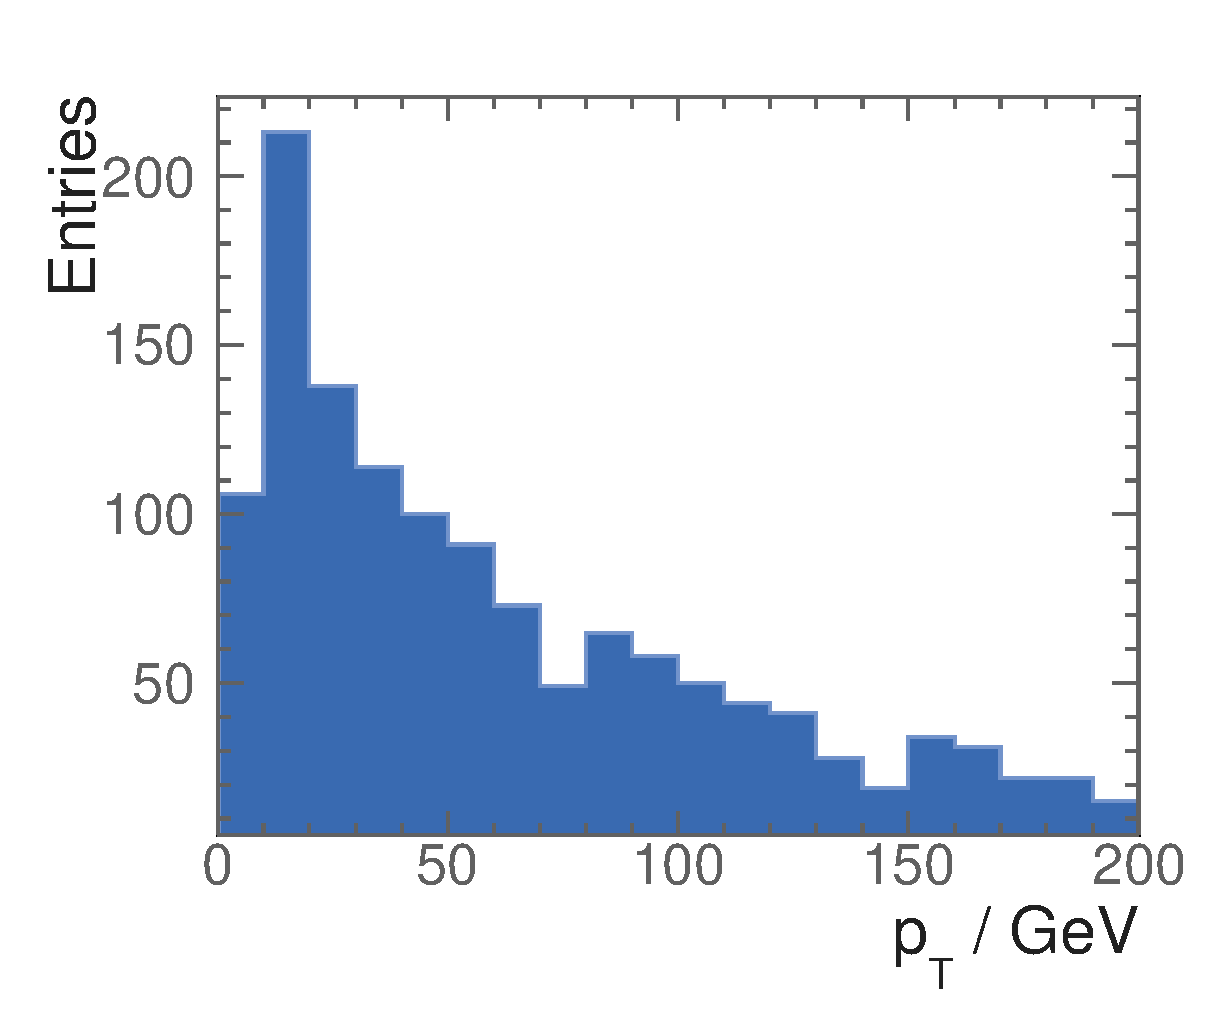
\includegraphics[width=\textwidth]{{{doubleHiggs/isoLep/electron1highPTbkg}}}
    \caption{}
    \label{fig:doubleHiggsBonoIsoLepE1HighPTBkg}
  \end{subfigure}
 \begin{subfigure}[b]{0.45\textwidth}
    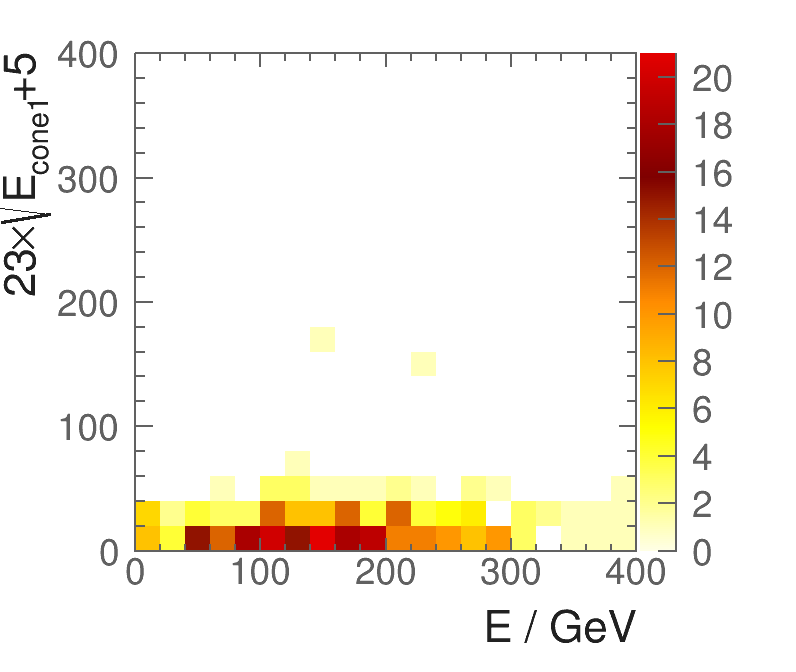
\includegraphics[width=\textwidth]{{{doubleHiggs/isoLep/electron1lowPTSignal}}}
    \caption{}
    \label{fig:doubleHiggsBonoIsoLepE1LowPTSgl}
  \end{subfigure}
  \begin{subfigure}[b]{0.45\textwidth}
    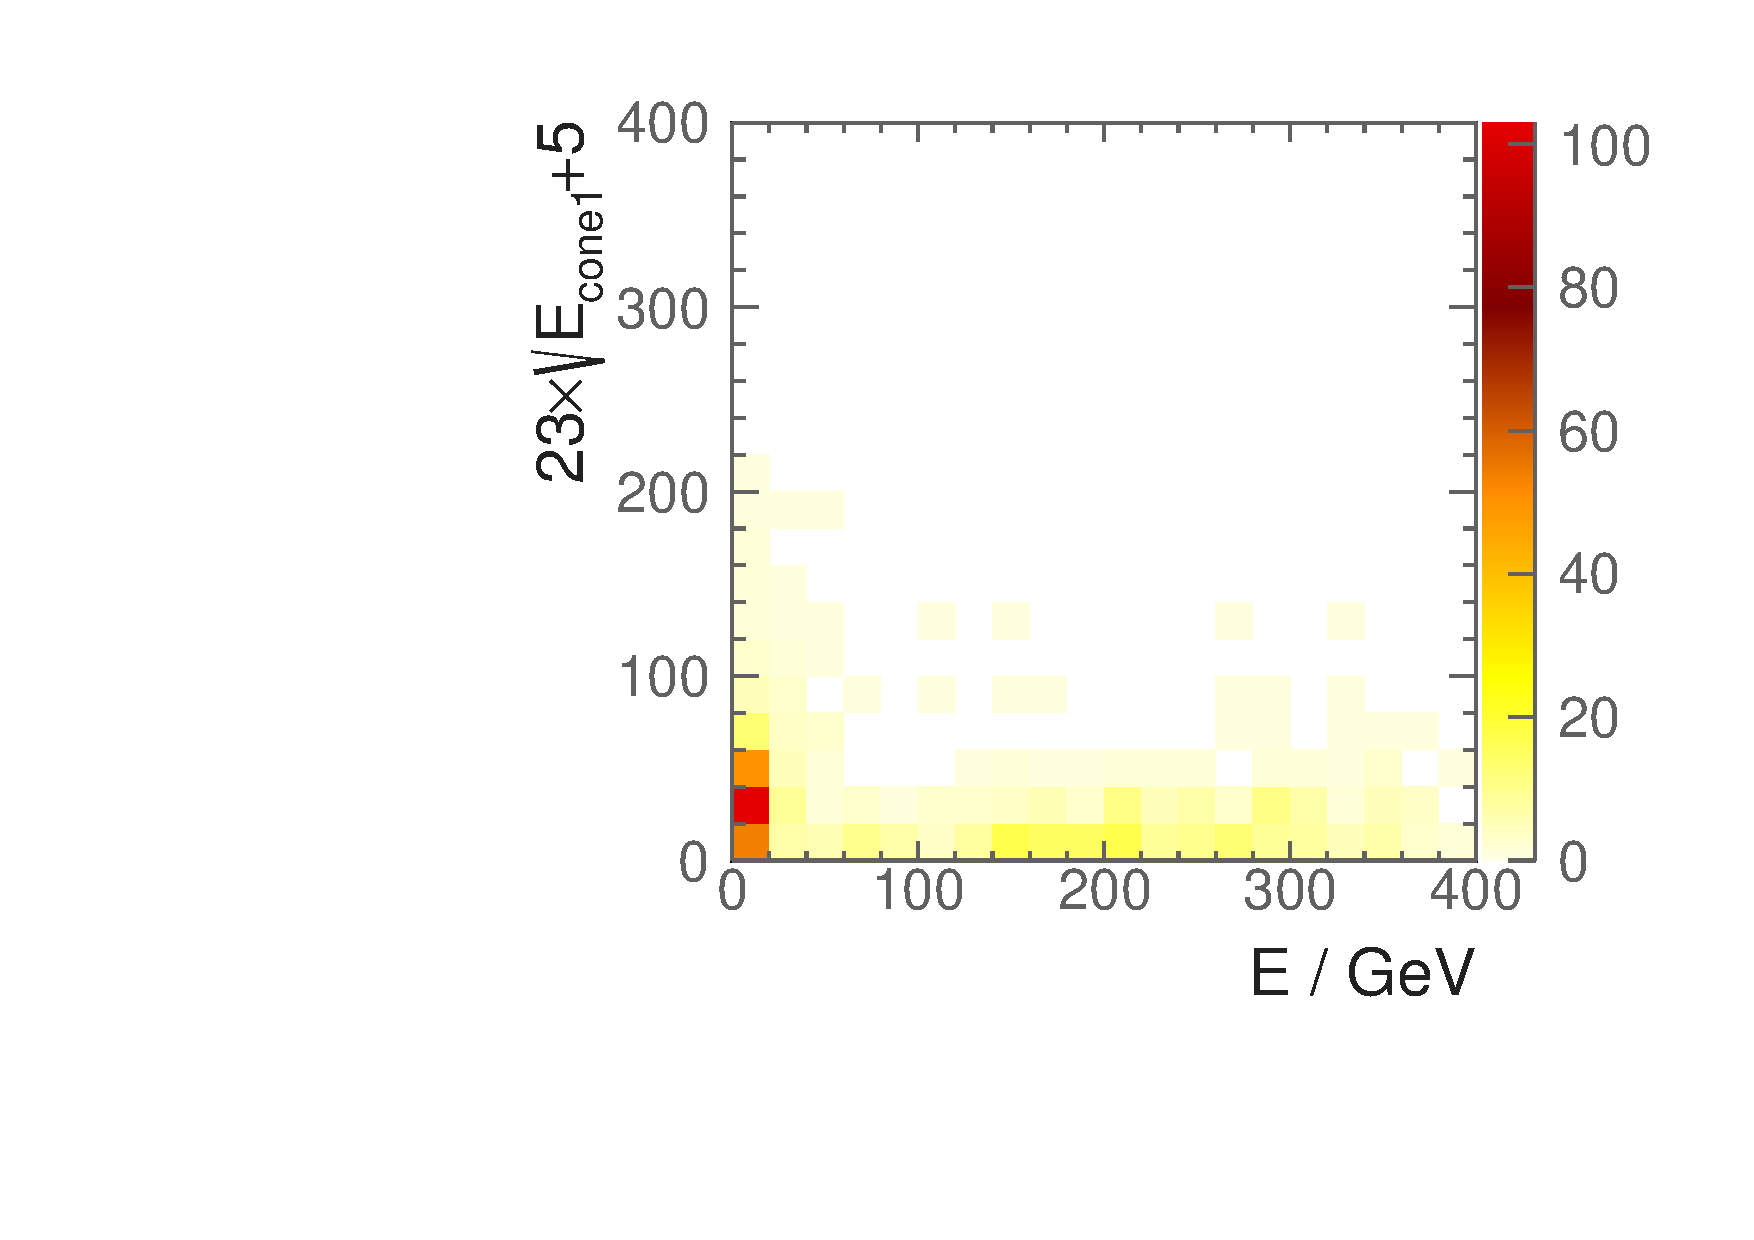
\includegraphics[width=\textwidth]{{{doubleHiggs/isoLep/electron1lowPTbkg}}}
    \caption{}
    \label{fig:doubleHiggsBonoIsoLepE1LowPTBkg}
  \end{subfigure}
\caption
   {Distributions shown for \pT  of identified electrons after  $E$  and $r_0$ cuts, for: a)  \eeToHHbbWWHad signal process; and b) \eeTo{ \Pquark \Pquark \Pquark \Pquark \Plepton \Pnu}  background process. Distributions shown for  $23\,\uprightMath{GeV^{\frac{1}{2}}} \times \sqrt{E_{cone1}} + 5\,\uprightMath{GeV}$ as a function of $E$  after  $E$  and $r_0$ cuts, for: c)  \eeToHHbbWWHad signal process; and d) \eeTo{ \Pquark \Pquark \Pquark \Pquark \Plepton \Pnu}  background process.}
   \label{fig:doubleHiggsBonoIsoLepE1}
\end{figure}


\begin{comment}
\subsubsection{Comparison: \IsolatedLeptonFinderProcessor versus \BonoLeptonFinder}

The two processors share similar criterion for light lepton identification. The main difference is that the \BonoLeptonFinder uses particle identification from \pandora, which takes into account extra calorimetric information to determine the particle ID than simple \ECAL energy fraction. \BonoLeptonFinder also allows high \pT light leptons to be identified in a non-isolated environment.
%aggressive nature of the \BonoLeptonFinder. %The performance of two processors on the signal and selected background samples is shown in \Table{tab:doubleHiggsIsoLepPerformance}.
\end{comment}

\subsection{Tau lepton identification}

The tau lepton has a short lifetime and decays before reaching the vertex detector and  can only be identified through the reconstruction of its decay products. The leptonic decay of tau lepton can be identified using the isolated lepton finder processors described above. Therefore in this section, tau identification will focus on the hadronic decay modes.

The existing \TauFinderProcessor  \cite{LCD-Note-2010-009} reconstruction package has been optimised. In addition, a package, \BonoTauFinder, was developed to provide additional tau lepton identification.

%To improve signal selection, a tau lepton identifier is developed by the author in \Section{sec:doubleHiggsBonoTauFinder}.



\subsubsection{\TauFinderProcessor}

The \TauFinderProcessor works by identifying tau lepton decay products, and requiring the decay products to be isolated from other PFOs. To find the decay products, the algorithm starts with the highest energy track as a seed for the cone clustering algorithm. A cone with opening angle 0.03 rad with respect to the seed is formed. The PFOs within the cone are required to be consistent with the signature of a tau hadronic decay: no more than 3 charged particles in the cone; invariant mass of all PFOs in the cone less than 2\,GeV; and few than 10 \PFOs in the cone. The cone is also required to be isolated from other particles. To reduce fake rate, PFOs with low momentum (less than 1\,GeV) are not used  in tau finding, as they more likely come from \ggHad background. The identified tau lepton and associated decay products are then not used in further tau finding. This tau lepton finding procedure iterates with other high-energy tracks as seeds.


The optimised parameters are listed in \Table{tab:doubleHiggsTauFinderProcessor}. The optimisation is performed by the collaborator using \eeToHHbbbb signal process and the \eeTo{ \Pquark \Pquark \Pquark \Pquark \Plepton \Pnu} background process, by scanning the parameters to obtain a good background rejection rate with lowest signal rejection rate.  Variables are defined in the same way as in previous sections. In addition: $\theta_Z$ is the polar angle with respect to the beam axis; $N_{X^+}$ and $N_{\Ptau}$ are the number of charged particles and the number of \PFOs  in the tau cone respectively; $m_{\Ptau}$ is the invariant mass of the sum of the PFOs in the tau candidate; and $E_{cone}$ is the total energy of \PFOs within a cone of an opening angle between 0.03 and 0.33\,rad  around tau seed track.

\begin{table}[!htbp]
\begin{tabular}{lr}
\hline
\hline
\TauFinderProcessor  & Selection \\
\hline
Veto \ggHad  &  $\pT < 1$\,GeV \\
Seed particle & $\pT > 10$\,GeV \\
Tau candidate cone opening angle & 0.03\,rad \\
Tau candidate rejection & $N_{X^+} > 3$;\, $N_{\Ptau} > 10$;\, $m_{\Ptau} > 2$\,GeV   \\
Isolation &  $ E_{cone} < 3$\,GeV\\
\hline
\hline
\end{tabular}
\caption
{Optimised parameters of the  \TauFinderProcessor processor.}
\label{tab:doubleHiggsTauFinderProcessor}
\end{table}

\subsubsection{\BonoTauFinder}
\label{sec:doubleHiggsBonoTauFinder}

The \BonoTauFinder works in a similar way to the \TauFinderProcessor. It identifies high momentum particles as tau seeds. Particles are iteratively added to a cone in the order of the ascending opening angle to the seed. The cone is called search cone, which contains potential tau decay products. After each particle addition, the temporary search cone is then considered as a temporary  tau candidate and tested for isolation and consistency  with a tau hadronic decay signature. The temporary tau candidate only needs to pass one of the isolation conditions to be identified as a tau candidate. There are multiple isolation conditions for tau 1-prong decay and 3-prong decay, reflecting different topologies of tau decay final states. The isolation criteria typically demand few particles around the search cone and the total \pT in the search cone to be greater than a threshold.

The iterative particle addition procedure stops when the cone opening angle is larger than a threshold. If multiple temporary tau candidates of the same tau seed pass the selection, the one with smallest opening angle is chosen to form the final tau candidate. To reduce the fake rate from \ggHad background, particles with energies less than 1\,GeV are not considered.


\TABLE{tab:doubleHiggsTauFinderProcessor} lists the optimised parameters  for \BonoTauFinder. Variables are defined in the same way as those in previous sections. In addition, $\theta_S$ is the opening angle of the search cone in rad; $cone1$ and $cone2$ are defined as a cone around the tau seed of an opening angle of $\cos^{-1}(0.95)$, and $\cos^{-1}(0.99)$ respectively.

\begin{table}[!htbp]
\begin{tabular}{lr}
\hline
\hline
\BonoTauFinder  & Selection \\
\hline
Veto \ggHad&  $E < 1$\,GeV\\
Seed particle & $\pT > 5$\,GeV \\
\multicolumn{1}{L{0.3\textwidth}}{Maximum search cone opening angle} & $\theta_S \leqslant \cos^{-1}(0.999)$\,GeV\\
Tau candidate rejection & $N_{X^+} \neq 1,3$;\, $m_{PFO} > 3$\,GeV   \\
\hspace{3mm} Isolation 1 or& $N_{cone1} = 0$;\, $ \pT_{cone} \geqslant 10$\,GeV\\
\hspace{3mm} Isolation 2 or& $N_{X^+} = 1$;\, $N_{cone1} = 1$;\, $r_0 > 0.01$\,mm\\
\hspace{3mm} Isolation 3 or& \multicolumn{1}{R{0.7\textwidth}}{{$N_{X^+} = 3$;\, $N_{cone1} = 1$;\, $ \pT_{cone} \geqslant 10$\,GeV;\, $\theta_S < \cos^{-1}(0.9995)$}}\\
\hspace{3mm} Isolation 4 or& \multicolumn{1}{R{0.7\textwidth}}{$N_{X^+} = 1$;\, $N_{cone2} = 0$;\, $r_0 > 0.01$\,mm;\, $ \pT_{cone} \geqslant 10$\,GeV}\\
\hspace{3mm} Isolation 5& \multicolumn{1}{R{0.7\textwidth}}{{$N_{X^+} = 3$;\, $N_{cone2} = 0$;\, $ \pT_{cone} \geqslant 10$\,GeV;\, $\theta_S < \cos^{-1}(0.9995)$}}\\
\hline
\hline

\end{tabular}
\caption
{Optimised parameters of \BonoTauFinder processor}
\label{tab:doubleHiggsBonoTauFinderProcessor}
\end{table}

\FIGURE{fig:doubleHiggsBonoIsoTau} shows the distributions of variables used in isolation criterion of tau candidate for \eeToHHbbWWHad signal process (blue) and  \eeTo{ \Pquark \Pquark \Pquark \Pquark \Plepton \Pnu}  background process (orange). \FIGURE{fig:doubleHiggsBonoIsoTau1} shows the distribution of the transverse momentum of the particles in the search cone, after selecting $N_{cone1} = 0$, used in the  isolation criterion 1. The cut at  $ \pT_{cone} \geqslant 10$\,GeV selects more tau candidates in background events than in the signal events, where there should be no true high-energy isolated tau leptons in signal events. Shown in \Figure{fig:doubleHiggsBonoIsoTau2}, after selecting $N_{X^+} = 1$ and $N_{cone1} = 1$,  the cut at $r_0 > 0.01$\,mm used in the isolation criterion 2 selects more true tau candidates in background events.  \FIGURE{fig:doubleHiggsBonoIsoTau1} shows the distribution of the transverse momentum of the particles in the search cone, after requiring  $N_{X^+} = 3$, $N_{cone1} = 1$ and $\theta_S < \cos^{-1}(0.9995)$ for  isolation criteria 3. The cut at $ \pT_{cone} \geqslant 10$\,GeV  selects  tau candidates in background events.


% of the isolation criteria 1, where  Similarly, in \Figure{fig:doubleHiggsBonoIsoTau2}, the cut at $r_0 > 0.01$\,mm, and in \Figure{fig:doubleHiggsBonoIsoTau3}, the cut at $ \pT_{cone} \geqslant 10$\,GeV


%tau hypothesis singular or tau hypotheses plural?


\begin{figure}[!htbp]
  \begin{subfigure}[b]{0.45\textwidth}
    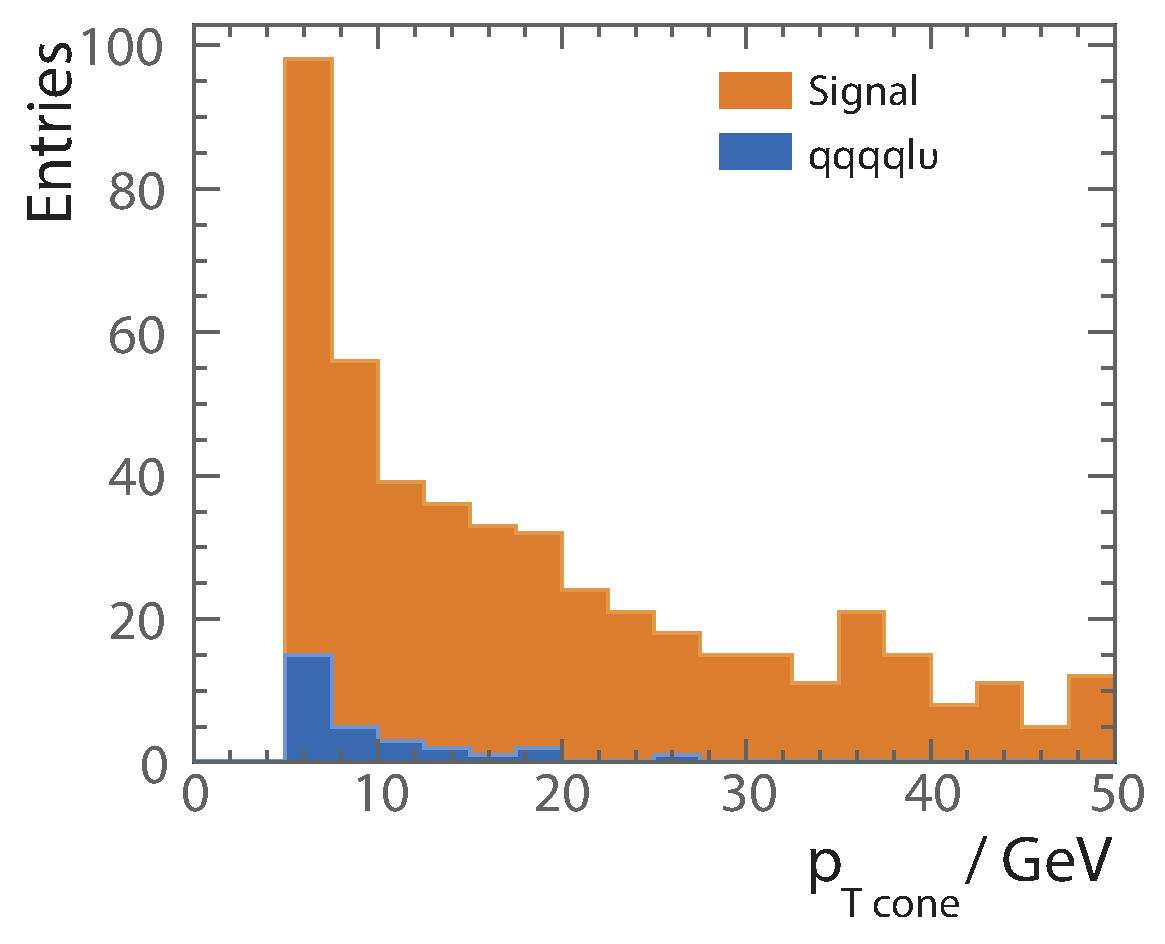
\includegraphics[width=\textwidth]{{{doubleHiggs/isoLep/tau1v2}}}
    \caption{}
    \label{fig:doubleHiggsBonoIsoTau1}
  \end{subfigure}
  \begin{subfigure}[b]{0.45\textwidth}
    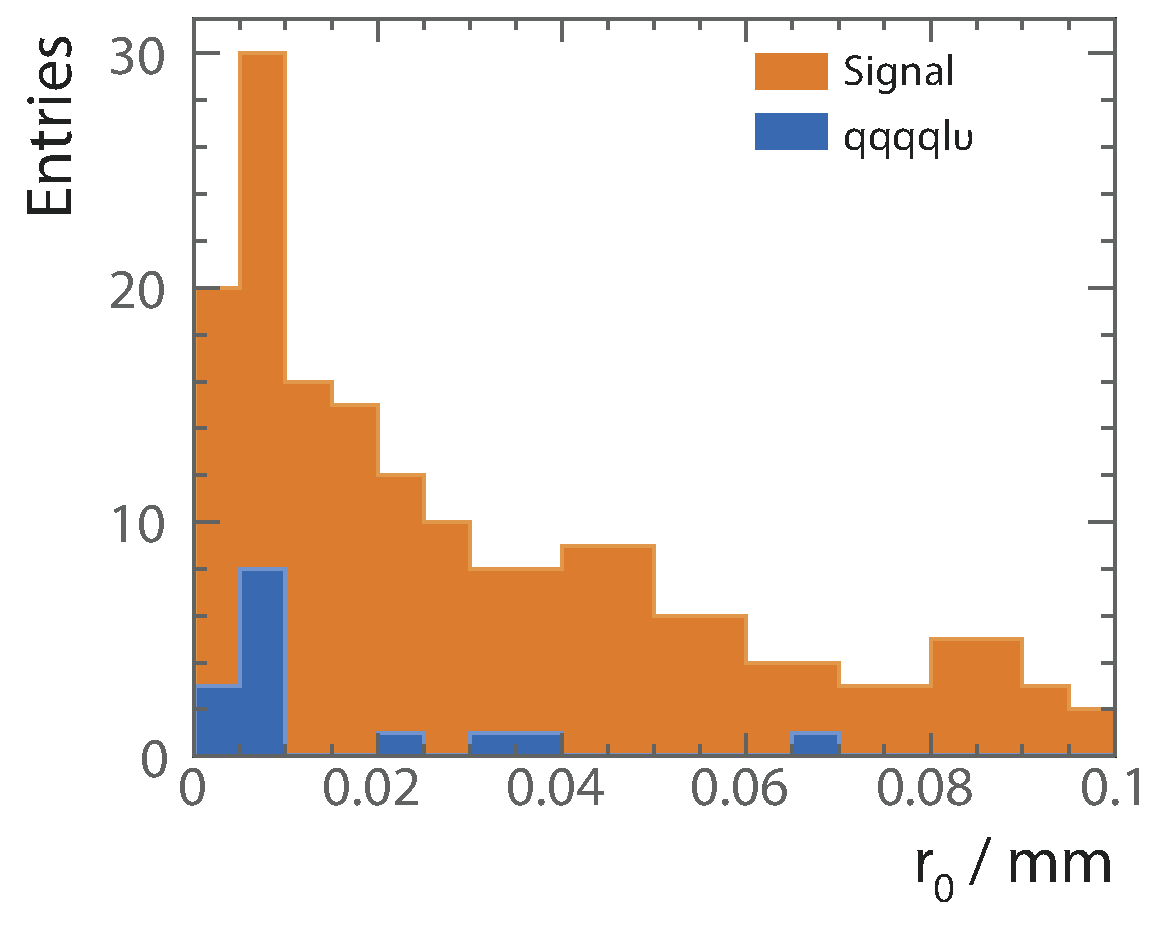
\includegraphics[width=\textwidth]{{{doubleHiggs/isoLep/tau2realv2}}}
    \caption{}
    \label{fig:doubleHiggsBonoIsoTau2}
  \end{subfigure}
 \begin{subfigure}[b]{0.45\textwidth}
    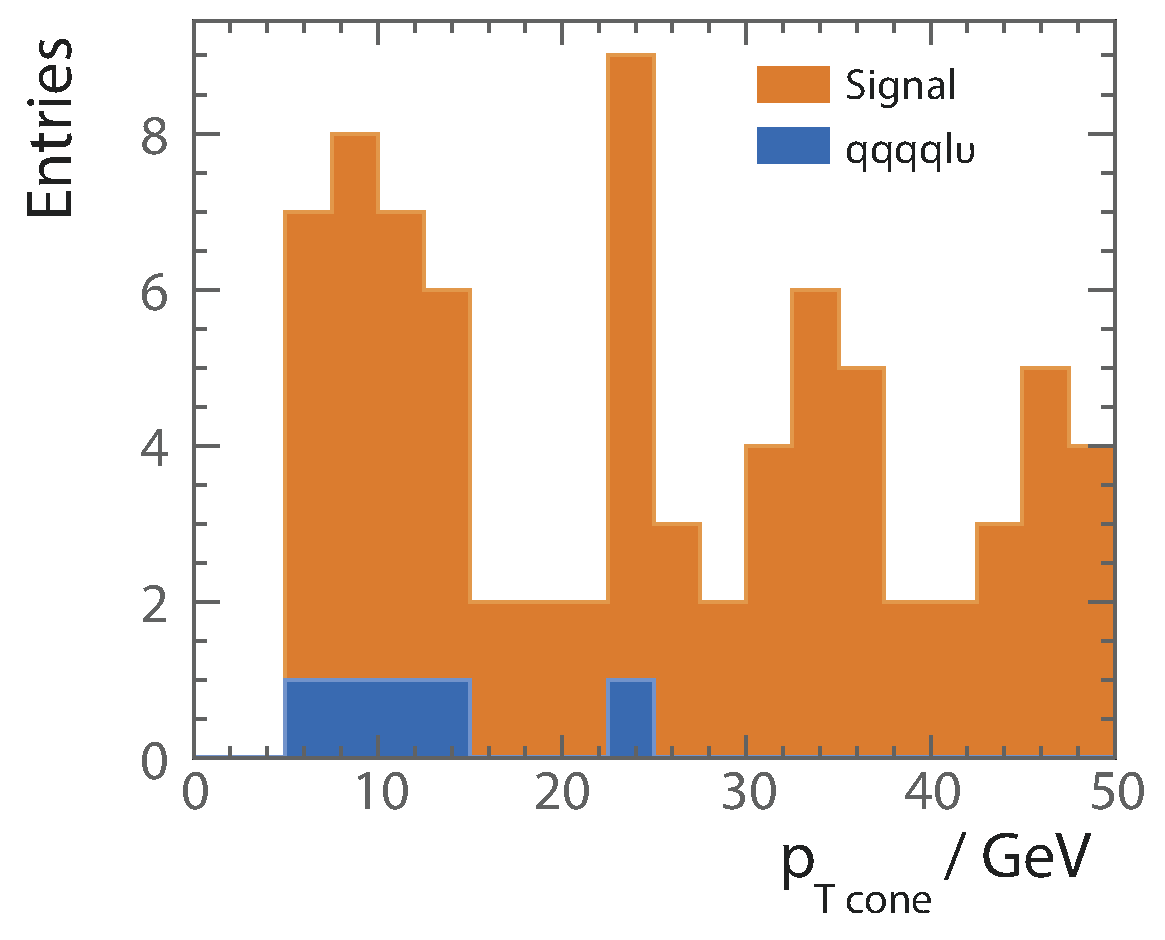
\includegraphics[width=\textwidth]{{{doubleHiggs/isoLep/tau3v2}}}
    \caption{}
    \label{fig:doubleHiggsBonoIsoTau3}
  \end{subfigure}
\caption
   { Distributions to show isolation criteria: a) $\pT_{cone}$ for isolation criterion 1  after  selecting $N_{cone1} = 0$;  b) $r_0$ for isolation criterion 2  after selecting $N_{X^+} = 1$, $N_{cone1} = 1$; and c) $\pT_{cone}$ for isolation criteria 3  after selecting  $N_{X^+} = 3$, $N_{cone1} = 1$, $\theta_S < \cos^{-1}(0.9995)$. Particle ID is from the truth information.  Distributions are shown for tau candidates in \eeToHHbbWWHad signal process (blue) and  \eeTo{ \Pquark \Pquark \Pquark \Pquark \Plepton \Pnu}  background process (orange).}
   \label{fig:doubleHiggsBonoIsoTau}
\end{figure}



Relative to the \TauFinderProcessor algorithm, the main difference is that the \BonoTauFinder adopts an iterative approach to build up a tau candidate, which allows a dynamic tau search cone size.

%The \BonoTauFinder also has smaller cut values on the minimum \pT and invariant mass of the tau candidate, but stricter isolation criterions.
%I've reworded the first sentence in this para - does it make sense?
%looser cut - is this the accepted term? if not, maybe replaced the word looser with something else


\subsection{Very forward electron identification}
\label{sec:doubleHiggsForwardElectron}


At the high centre-of-mass energy of \CLIC, particles produced are often highly boosted.  Because of this, it is important to identify leptons in the forward calorimeters to aid the signal selection. In particular, photon$-$electron interactions can have energetic primary  electrons in  the forward calorimeters, the \LumiCAL and/or the \BeamCAL.

Because of the large background in the forward region, it is challenging to identify primary leptons. In the Monte Carlo production, particles including the primary leptons and beam induced background in the forward calorimeters are not simulated, due to the high demand on the computational resources. Instead, studies have been performed with particles simulated in the forward calorimeters to understand the primary lepton identification efficiencies \cite{sailer2012radiation,Sailer:2017onh,Lukic:forwardElectron}. The studied  primary lepton identification efficiencies are then parameterised as a function of lepton energies. The parametrisation approach is adopted in this analysis.

\FIGURE{fig:doubleHiggsForwardBCAL} shows the primary electron identification efficiencies in the \BeamCAL as a function of polar angle for a 500\,GeV electron.  An external processor \cite{Sailer:2017onh} has been developed to parameterise the primary electron identification efficiencies in the \BeamCAL at \rootS{3} as a function of electron energy and the polar angle. The full simulation study to obtain the primary electron identification efficiencies in the \BeamCAL assumes a background integrated over 40 bunch crossings.  The same primary electron identification efficiency is assumed for \rootS{1.4} and \rootS{3}. In the analysis for \rootS{1.4}, the momenta of the electron is scaled down by a ratio of the centre-of-mass energies to use the external processor.

\FIGURE{fig:doubleHiggsForwardLCAL} shows the primary electron identification efficiencies in the \LumiCAL as a function of electron energy for a polar angle $\theta = 50$\,mrad. The efficiency is obtained from a full simulation study \cite{Lukic:forwardElectron}, assuming a background integrated over 100 bunch crossings. In this analysis, the primary electron identification efficiency  as a function of electron energy is assumed to be parameterised by the curve in \Figure{fig:doubleHiggsForwardLCAL}. The polar angle dependency of the efficiency is not considered, due to the lack of study. The primary electron identification efficiency curve in \Figure{fig:doubleHiggsForwardLCAL} takes the functional form of:
\begin{equation}
\varepsilon=
\begin{cases}
  0, & \text{if}\ E < 50\,\text{GeV},\\
  0.99 \times \frac{(erf(E / \text{GeV} - 100) + 1 )}{2}, & \text{otherwise},
\end{cases}
\end{equation}
where $E$ is the energy of the electron and $erf$ is the error function.

Due to a lack of tracking detector in the very forward region, electrons and photons can not be differentiated. Therefore, both photons and electrons are identified in the forward calorimeters. Events with identified high-energy electrons and/or photons in the \BeamCAL and/or \LumiCAL are rejected.

%For each MC electron in the \LumiCAL, a random number between 0 and 1 is generated. If the random number is less than \varepsilon, the MC electron is tagged.

%It is important to identify leptons in the forward calorimeters to aid the signal selection because  certain background channels, for example



%At the high centre-of-mass energy at the \CLIC, particles are often boosted.  It is important to identify leptons in the forward calorimeters to aid the signal selection because  certain background channels, for example photon-electron interactions, can have energetic primary  electrons in  the forward calorimeters, the \LumiCAL and/or the \BeamCAL.

%It is challenging to identify electrons in these forward calorimeters.  Most particles in these forward calorimeters are from the beam induced background. Nevertheless, sufficiently high energy electrons can be efficiently identified in the \BeamCAL   and \LumiCAL \cite{sailer2012radiation}.
\begin{comment}
The high charge density in the bunches will induce strong electromagnetic fields causing deflection of the
beam particles and the radiation of
beamstrahlung
. In addition, the beamstrahlung photons will interact
with the beam particles and produce electron–positron and quark–anti-quark pairs.  While the photonic
component will be radiated practically along the outgoing beam axis, a noticeable fraction of leptonic
and hadronic pairs will hit the BeamCal calorimeter in the forward region.
\end{comment}

%The reconstruction of electrons in the forward calorimeters uses  a parametrisation approach.  By parameterising the  particle ID efficiency using MC particles, the equivalent performance to the full detector simulation approach can be achieved \cite{Sailer:2017onh,Lukic:forwardElectron} .

%For the \CLICILD detector concept, energies deposited in the \LumiCAL and the \BeamCAL are not reconstructed in simulation. This is because the thousands of beam induced background particles per bunch crossing requires expensive computational resources. However, previous studies \cite{Sailer:2017onh,Lukic:forwardElectron} using parameterise the particle ID efficiency using MC particles give equivalent performance to the full detector simulation approach.


%The current simulation software could not handle the simulation in a feasible time. Therefore, the adopted approach is to parameterise the background particle energy deposition leading to electron tagging algorithms.
%I changed 'and leads to' to 'leading to'. Is that what you meant? The original text was mixing tenses

%For the \BeamCAL, an existing electron tagging algorithm was developed using \rootS{3} collision environment by comparing the simulated electron and background energy distributions \cite{Sailer:2017onh}. An indicative performance plot of 500\,GeV electron tagging efficiency as a function of polar angle is shown in \Figure{fig:doubleHiggsForwardBCAL}. An electron is tagged if the energy is significantly larger than the expected background energy distributions integrated over 40 bunch crossing.

%This parametric tagging approach  most likely underestimates efficiencies due to the coarse binning of energies. For example,  a 650\,GeV particle is treated in the same way as a 600\,GeV particle, as the tagging efficiency for electrons with energy 500 to 1500\,GeV are binned in histograms at an interval of 100\,GeV. Also there is no tagging efficiency for electrons with energy below 500\,GeV or above 1500\,GeV.


%A C++ code library has been developed and used in this analysis.

%The input of the \BeamCAL electron tagging algorithm is the four momenta of the MC electron. Since the algorithm assumes collisions at \rootS{3}, for the \rootS{1.4} user case, the momenta of the MC electron is scaled down by a factor of $\frac{3}{1.4}$.



%For the \LumiCAL,  \Figure{fig:doubleHiggsForwardCAL} shows the \LumiCAL  electron tagging efficiency as a function of the electron energy for polar angle $\theta = 50$\,mrad where events are overlaid with background energy deposition integrated over 100 bunch crossings \cite{Lukic:forwardElectron}. In this analysis, the \LumiCAL electron tagging efficiency, $\varepsilon$, is parameterised as

%Assuming that the \LumiCAL electron tagging efficiency in this analysis is the same as in \Figure{fig:doubleHiggsForwardCAL} for all polar angles and for \rootS{1.4} and 3\,TeV,
%The \LumiCAL electron tagging in this analysis is based on the performance plot in \Figure{fig:doubleHiggsForwardCAL}.

%the \HepProcess{\PHiggs \to \Pmu \Pmu} analysis in \cite{Milutinovic-Dumbelovic:2014uta,Grefe:2012rt} has developed an algorithm for electron tagging in the \LumiCAL with similar logic to the algorithm for the \BeamCAL.
% as this is the only study available for comparison.


\begin{figure}[!htbp]
  \begin{subfigure}[b]{0.45\textwidth}
    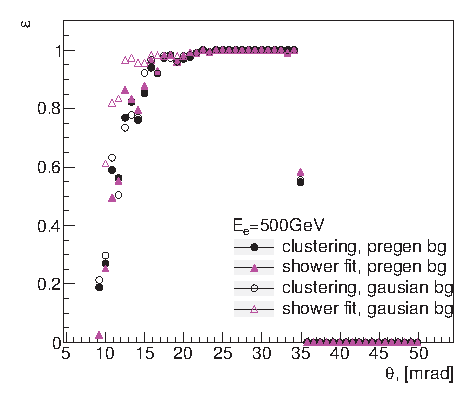
\includegraphics[width=\textwidth]{{{doubleHiggs/forward/ForwardBCAL}}}
    \caption{}
    \label{fig:doubleHiggsForwardBCAL}
  \end{subfigure}
  \begin{subfigure}[b]{0.45\textwidth}
    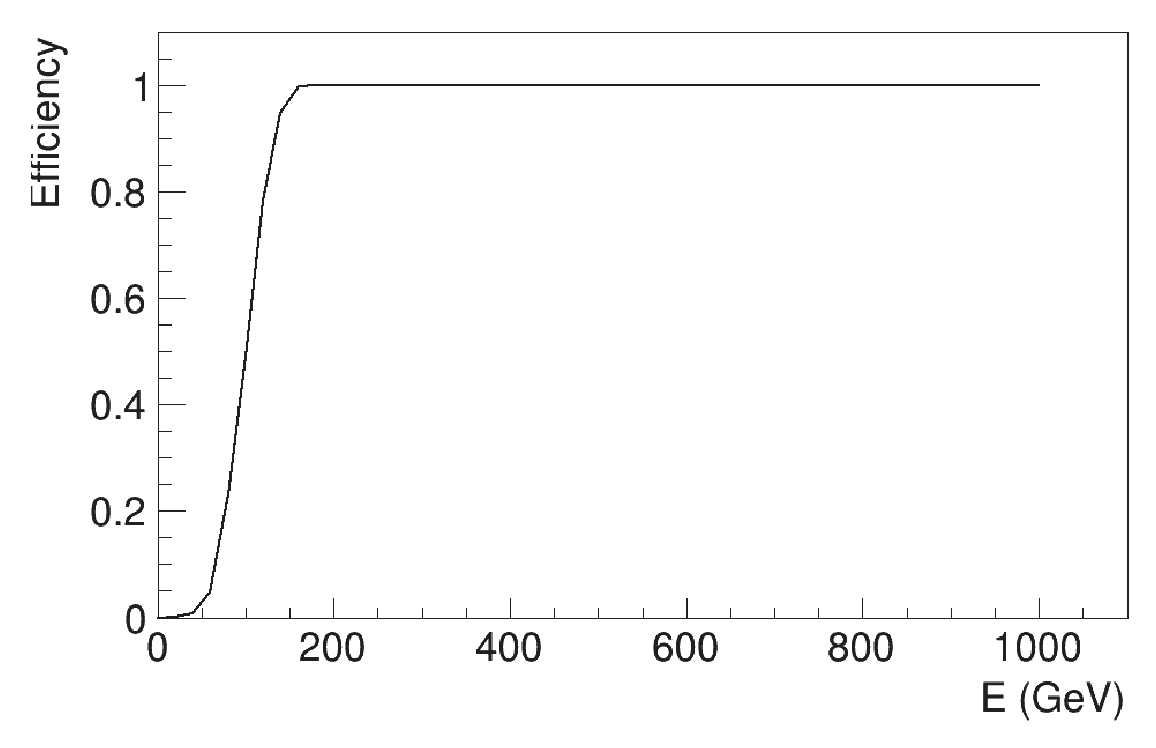
\includegraphics[width=\textwidth]{{{doubleHiggs/forward/ForwardLCAL}}}
    \caption{}
    \label{fig:doubleHiggsForwardLCAL}
  \end{subfigure}
\caption[\BeamCAL and \LumiCAL electron tagging efficiency.]%
   {a) 500\,GeV electron identification efficiency in the \BeamCAL as a function of polar angles, with different methods to model backgrounds: pregenerated and Gaussian,  and two methods to identify electrons:  clustering algorithm and  shower fitting algorithm, obtained from a full simulation study in \cite{Sailer:2017onh}. b)  electron tagging efficiency in the \LumiCAL as a function of the electron energy, for a polar angle $\theta = 50$\,mrad, obtained from a full simulation study in  \cite{Lukic:forwardElectron}. }
   \label{fig:doubleHiggsForwardCAL}
\end{figure}

%appear indistinguishable to the \BeamCAL and \LumiCAL and both photons and electrons are tagged by the above algorithms.


 %Due to the lack of tracking in these region, electrons and photons would have the same electromagnetic shower profile, with the given calorimeter resolution. MC photons and electrons are checked if they fall in the LCal or the BCal, and checked against the known detection efficiency.


%With the increase of the centre-of-mass energy, more  As discussed before, veto events with leptons help the signal selection. Hence the goal is to identify leptons in the forward region.

%These forward calorimeters were not simulated due to computational limitation.
% For \rootS(3), the BeamCal detection efficiency is provided by a software package \cite{}. For \rootS(1.4), the same software for the BeamCal is used, by scaling the energy of the MC particle by a factor of $\frac{3}{1.4}$. For the LumiCal, the identification efficiency is defined as


\subsection{Lepton identification performance}

The performances of the different lepton finding processors for signal events and the selected background processes are shown in \Table{tab:doubleHiggsIsoLepPerformance} for \rootS{1.4}. Numbers in the table  represent the fractions of events  where no leptons are identified by the individual lepton finder.  \BonoLeptonFinder and \BonoTauFinder reject more background events than the \IsolatedLeptonFinderProcessor and \TauFinderProcessor. By combining the processors, 86.6\% of the signal events remain and 16.8\% of the \HepProcess{\Pep \Pem \to \Pquark\Pquark\Pquark\Pquark\Plepton\Pnu} events survive after rejecting events where leptons are identified.
%Second sentence: can you say "" becase this would read better
% \TABLE{tab:doubleHiggsIsoLepPerformance} shows the performance of the processors for signal events and the  \egamma{\Pem}{\Pphoton}{BS}{\Pem \Pquark \Pquark \Pquark \Pquark} background events.

The forward lepton finders are most effective at rejecting background events with primary leptons in the forward region. Only 1\% of signal events are rejected, but 47.4\% of the \egamma{\Pem}{\Pphoton}{BS}{\Pem \Pquark \Pquark \Pquark \Pquark} background events are rejected.

%\TABLE{tab:doubleHiggs1.4TeVPreslection} list the number of events surviving lepton rejection for signal and all background channels.

\begin{table}[!htbp]
\begin{tabular}{lrrr}
\hline
\hline
Efficiency (1.4\,TeV)  &  Signal & \HepProcess{\Pep \Pem \to \Pquark\Pquark\Pquark\Pquark\Plepton\Pnu} & \egamma{\Pem}{\Pphoton}{\BS}{\Pem \Pquark \Pquark \Pquark \Pquark} \\
\hline
\IsolatedLeptonFinderProcessor & 99.3\% & 50.3\%  & 87.3\% \\
\BonoLeptonFinder & 99.1\% & 39.9\%  & 83.7\%\\
\TauFinderProcessor & 97.5\% & 52.3\%  & 90.4\% \\
\BonoTauFinder & 89.7\% & 38.5\%  &  78.5\% \\
Forward Finder Processors & 98.9\% & 95.1\%  & 53.6\% \\
\hline
Combined & 86.6\% & 16.8\%  &  30.8\% \\
\hline
\hline

\end{tabular}
\caption{The performances of the lepton finding algorithms for the signal events and selected background events at \rootS{1.4}.  \Pphoton(BS) represents a real photon from beamstrahlung (BS). Numbers represent the fractions of events where no leptons are identified by the individual lepton finder.}
\label{tab:doubleHiggsIsoLepPerformance}
\end{table}


The lepton finding processors were optimised with events at \rootS{1.4}.  It was found that the same set of parameters is also effective for \rootS{3}. The performances of the lepton finders at \rootS{3} are shown in \Table{tab:doubleHiggs3TeVIsoLepPerformance}.



%Would this read better if you explained why 1.4 is better rather than why 3 is worse? Better should be the focus, no?
When comparing the lepton finding performances at \rootS{1.4} and \rootS{3}, the performance for \rootS{1.4} is better. This is because at \rootS{3}, particles tend to be boosted more and the spatial separation between particles is smaller due to the higher multiplicities. Consequently particles are less isolated from each other. The higher centre-of-mass energy also affects the performance of the forward lepton finder. Whilst at \rootS{1.4}, the forward finder only rejects 5\% of the \HepProcess{\Pep \Pem \to \Pquark\Pquark\Pquark\Pquark\Plepton\Pnu} background events and 1\% of the signal events, at \rootS{3} it rejects 19\% of events from the same background process and 4\% of the signal events, as more leptons are boosted into the forward region.


\begin{table}[!htbp]
\begin{tabular}{lrrr}
\hline
\hline
Efficiency (3\,TeV)  &  Signal  & \HepProcess{\Pep \Pem \to \Pquark\Pquark\Pquark\Pquark\Plepton\Pnu}  & \egamma{\Pem}{\Pphoton}{\BS}{\Pem \Pquark \Pquark \Pquark \Pquark}  \\
\hline
\IsolatedLeptonFinderProcessor & 99.5\% & 66.8\% & 88.8\%  \\
\BonoLeptonFinder & 99.0\% & 52.5\%  & 82.2\%\\
\TauFinderProcessor & 97.7\% & 79.5\%  & 76.7\%\\
\BonoTauFinder & 86.3\% & 60.3\%  & 92.6\% \\
Forward Finder Processors & 95.9\% & 80.7\%  & 55.4\%  \\
\hline
Combined & 81.0\% & 23.3\% &  33.4\% \\
\hline
\hline

\end{tabular}
\caption{The performances of the lepton finding algorithms for the signal events and selected background events at \rootS{3}.  \Pphoton(BS) represents a real photon from beamstrahlung (BS). Numbers represent the fractions of events where no leptons are identified by the individual lepton finder.}
\label{tab:doubleHiggs3TeVIsoLepPerformance}
\end{table}


\begin{comment}
\begin{table}[!htbp]
\begin{tabular}{lrr}
\hline
\hline
Selection / Efficiency (1.4\,TeV)  &  Signal & \egamma{\Pem}{\Pphoton}{BS}{\Pem \Pquark \Pquark \Pquark \Pquark}  \\
\hline
Combined light lepton finder & 87.6\% & 67.5\%  \\
Forward Finder Processors & 98.9\% & 53.6\%  \\
\hline
Combined & 86.6\% & 30.8\%  \\
\hline
\hline

\end{tabular}
\caption{Very forward electron and photon finder performance on the signal and selected background events at \rootS{1.4}.}
\label{tab:doubleHiggsForwardPerformance}
\end{table}


\subsection{Other lepton identification processors}


Other isolated lepton identification processors have been tested, including IsolatedLeptonTagging and TauJetClustering. They either performed poorly comparing to the processors above, or became redundant after using the processors above. Therefore, these lepton identification processors are not used in this analysis.
%ATTN: does calibration/optimisation work better than tuning parameters?
\end{comment}

\section{Jet reconstruction}

The signal process, \eeToHHbbWWHad, is a six-quark final state, which will result in multiple reconstructed jets. The pairing of jets to form the \PH, \PWplus and \PWminus in the event is an essential part of the event reconstruction. In this section, the optimisation of the jet reconstruction is discussed.



% A useful technique for the analysis is to reconstruct the multi-jet final state using jet algorithms. This allows discriminative variables to be calculated. A brief discussion about jet algorithms and its relevance for the \CLIC and this analysis are provided.

\subsection{Jet reconstruction optimisation}
\label{sec:doubleHiggsJetOptimisation}

Jet reconstruction algorithms cluster particles into jets. For this analysis, longitudinal invariant \kt jet algorithm is chosen for the jet clustering, as discussed in \Section{sec:pandoraJetAlg}. The free parameter for \kt algorithm is the $R$ parameter, which controls the radius of the jet. The optimal jet clustering will also depend on the centre-of-mass energy of the event. This is particularly important at \CLIC because of the large beam induced background from relative low  \pT particles. Hence a suitable level of background suppression needs to be chosen, which is incorporated in the choice of the \PFO  collection.

%another choice affecting the jet reconstruction is the choice of the \PFO collection, which incorporates different level of timing and \pT cuts to reduce the beam induce background (see \Section{sec:pandoraggHad}).
%Both parameters are optimised for \rootS{1.4} and \rootS{3}.

The use of the \kt jet algorithm in exclusive modes allows some particles to be clustered into beam jet, which is not used in the subsequent event reconstruction.

The value of the $R$ parameter and the \PFO collection are chosen to optimise the invariant mass and mass resolution of \PHiggs and \PW. To choose the optimal parameters, \eeToHHbbWWHad events  are processed through \kt jet algorithm  in the six-jet exclusive mode. The six jets are paired using the MC truth information by examining the decay chain of MC particles. Four invariant mass distributions are obtained: two Higgs masses ($m_{\Hbb}$ and $m_{\HWW}$) and two \PW masses ($m_{\PW}$ and $m_{\W*}$). Here \W* indicates the off-mass-shell \PW boson. The MC paring is used to optimise the choice of parameters. It is not used in the subsequent analysis.

%The metric for optimising the $R$ parameter, and the \PFO collection, is the invariant mass and mass resolution of \PHiggs and \PW. An optimised jet reconstruction is chosen such that invariant masses of \PHiggs and \PW are close to their true masses, and invariant mass widths are small.

%For the jet reconstruction optimisation, only signal events are used and jets are paired to using MC truth information (see \Section{sec:pandoraMCtruthLink}).

%The sample for the optimisation is \eeToHH.

%The signal channel, hadronic decay of , is used for the jet reconstruction optimisation. The signal
%The six jets are paired up using  MC truth information to the corresponding Higgs and \PW boson.
%I'm not sure this last sentence is worded correctly. Doesn't make sense to me but I'm not a physicist!

%An example of $m_{\Hbb}$ invariant mass distribution is shown in .  Although the underlying mass distribution of particles like $m_{\PW}$ is a Breit-Wigner distribution, the overall mass distribution is Gaussian like, as the overall mass distribution is a convolution of a narrow \PW Breit-Wigner distribution and a wide Gaussian distribution for the detector resolution. The $m_{\Hbb}$  mass distribution is gaussian like but with asymmetrical width, due to \Pbottom quarks decaying to neutrinos, leading to a loss of detectable particles.
%\paragraph{Mass resolution fit}
Three invariant mass distributions are considered:  $m_{\Hbb}$, $m_{\HWW}$, and $m_{\PW}$. The optimal jet reconstruction should produce sharp mass peaks around the simulated particle masses. For example, \Figure{fig:doubleHiggsFitMCMass} shows the $m_{\Hbb}$ invariant mass distribution for $R = 1.3$ using the loose \PFO collection for samples at \rootS{3}. An analytical functional form is fitted to describe the shape. The fitting function is a Gaussian-like function. Additional parameters are used in the fitting function to describe the tails of the  distribution. The fitting function takes the form of
\begin{equation}
f(m)=A \exp\braces{- \frac{(m - \mu)^2}{g}},
\end{equation}
\begin{equation}
g=
\begin{cases}
2\sigma_L + \alpha_L(m - \mu), & \text{if}\ m < \mu,\\
2\sigma_R + \alpha_R(m - \mu), & \text{if}\ m \geqslant \mu,
\end{cases}
\end{equation}
where: $\mu$ is the fitted mass peak position; $\sigma_L$ and $\sigma_R$ allow for an asymmetrical width of the distribution; $\alpha_L$ and  $\alpha_R$  account for a constant tail of the distribution; and $A$ is a normalisation factor.


\begin{figure}[!htbp]
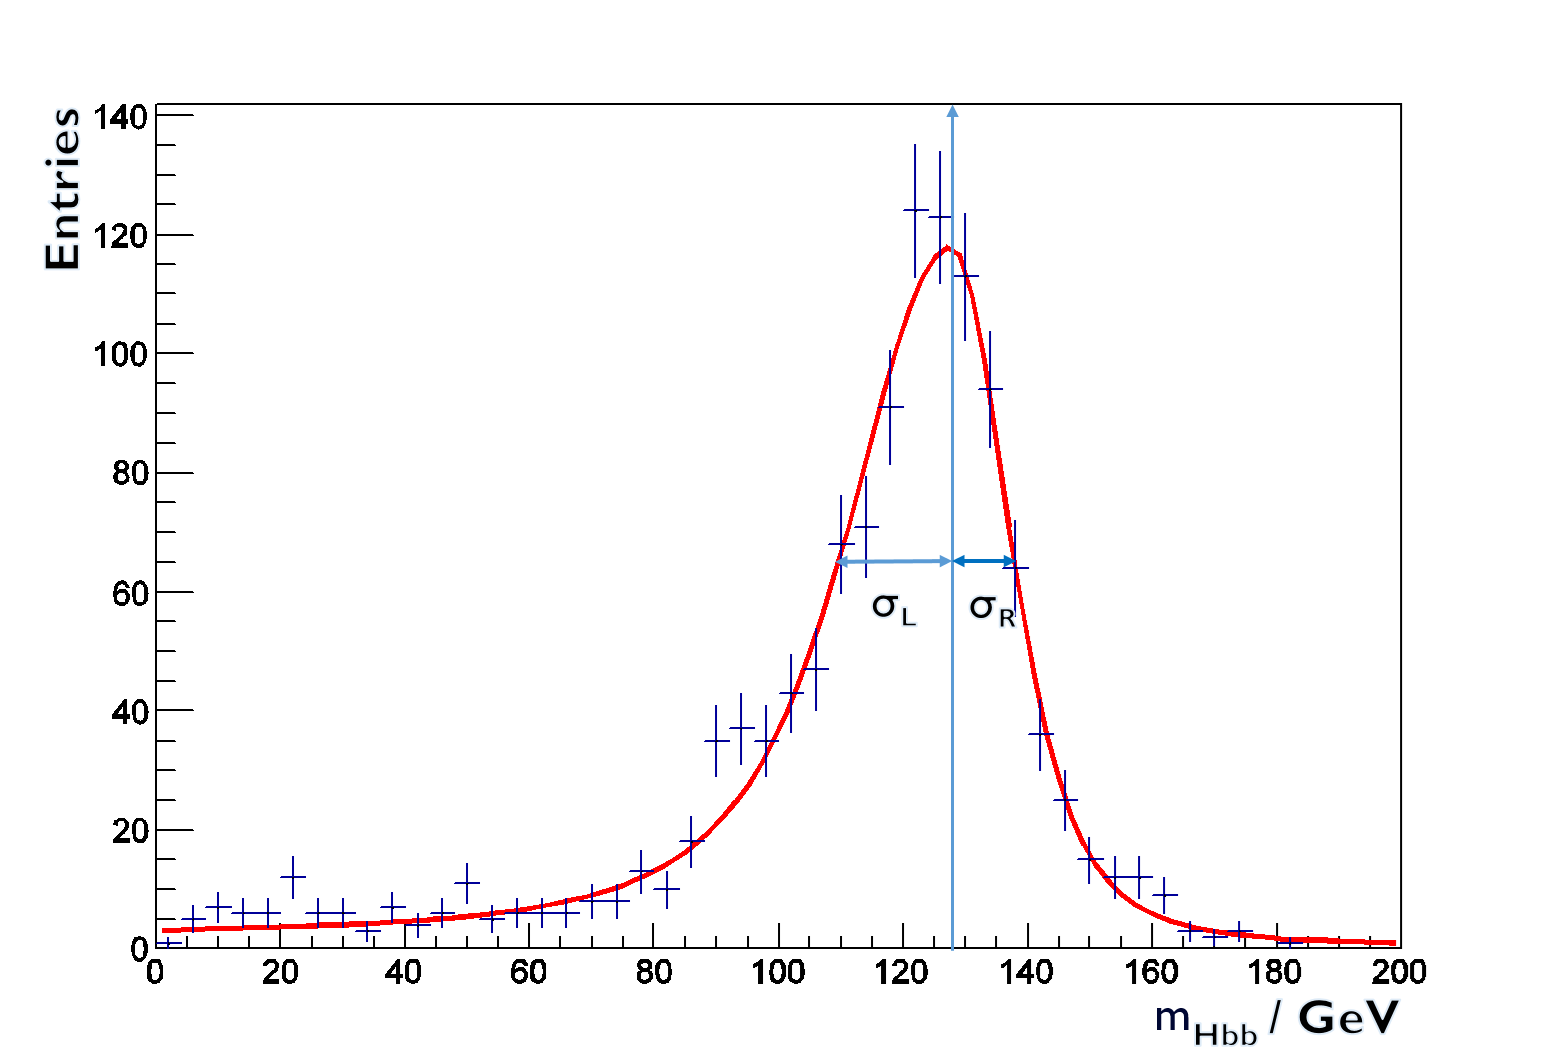
\includegraphics[width=\largefigwidth]{doubleHiggs/MCmassFit2}
\caption[Example MC mass fit for jet optimisation in double Higgs analysis]%
   {A typical example of the reconstructed $m_{\Hbb}$  mass distribution for $R$ = 1.3 using loose PFO collection for \eeToHHbbWWHad samples at \rootS{3}.  The fitting function is superimposed in red. The arrow shows the fitted peak position. }
   \label{fig:doubleHiggsFitMCMass}
\end{figure}

%\paragraph{Optimal $R$ and \PFO collection}

%The mass fit is performed for $m_{\Hbb}$, $m_{\HWW}$, and $m_{\PW}$ distributions.  The optimal jet reconstruction should have the mass peak close to the particle's simulated mass and a narrow peak width.
To parameterise the performance of different jet algorithm settings, the overall relative width is used, defined as $\left(\sigma_L  + \sigma_R\right)/M$. A smaller width indicates a  better mass resolution. The fitted \Hbb, \HWW, and \PW masses are studied for $R$ values between 0.5 and 1.3, and with the three possible \PFO collections: loose, normal, and tight.


\FIGURE{fig:doubleHiggs1.4TeVMassFit} shows the variation of the mass peak position and its relative width as a function of $R$ and \PFO collections, for $m_{\Hbb}$, $m_{\HWW}$, and $m_{\PW}$. The mass peak position, $\mu$, increases as $R$ increases. This is because more particles are included in jets with increasing jet radii. For the relative width, the values for \Hbb  increase with increasing jet radii, but the values for \HWW decrease  with increasing jet radii. This is due to a compensating effect; the invariant mass for \HWW is formed from four jets, which prefers a large jet radius, whereas the invariant mass for \Hbb is obtained from two jets, which favours a small jet radius.

The choice of \PFO collection impacts number of \PFOs in the event. The loose \PFO selection has the most \PFOs in the event and, therefore, the largest invariant mass and worst mass resolution.

Based on the results summarised in \Figure{fig:doubleHiggs1.4TeVMassFit} for this analysis, it was decided to use  $R = 0.7$  with the \normalPFO. This choice  gives good fitted mass peak positions for \Hbb, \HWW and \PW. The extracted fitted parameters of optimal jet reconstructions are summarised in \Table{tab:doubleHiggsFitParameters}.

\begin{figure}[!htbp]
  \begin{subfigure}[b]{0.45\textwidth}
    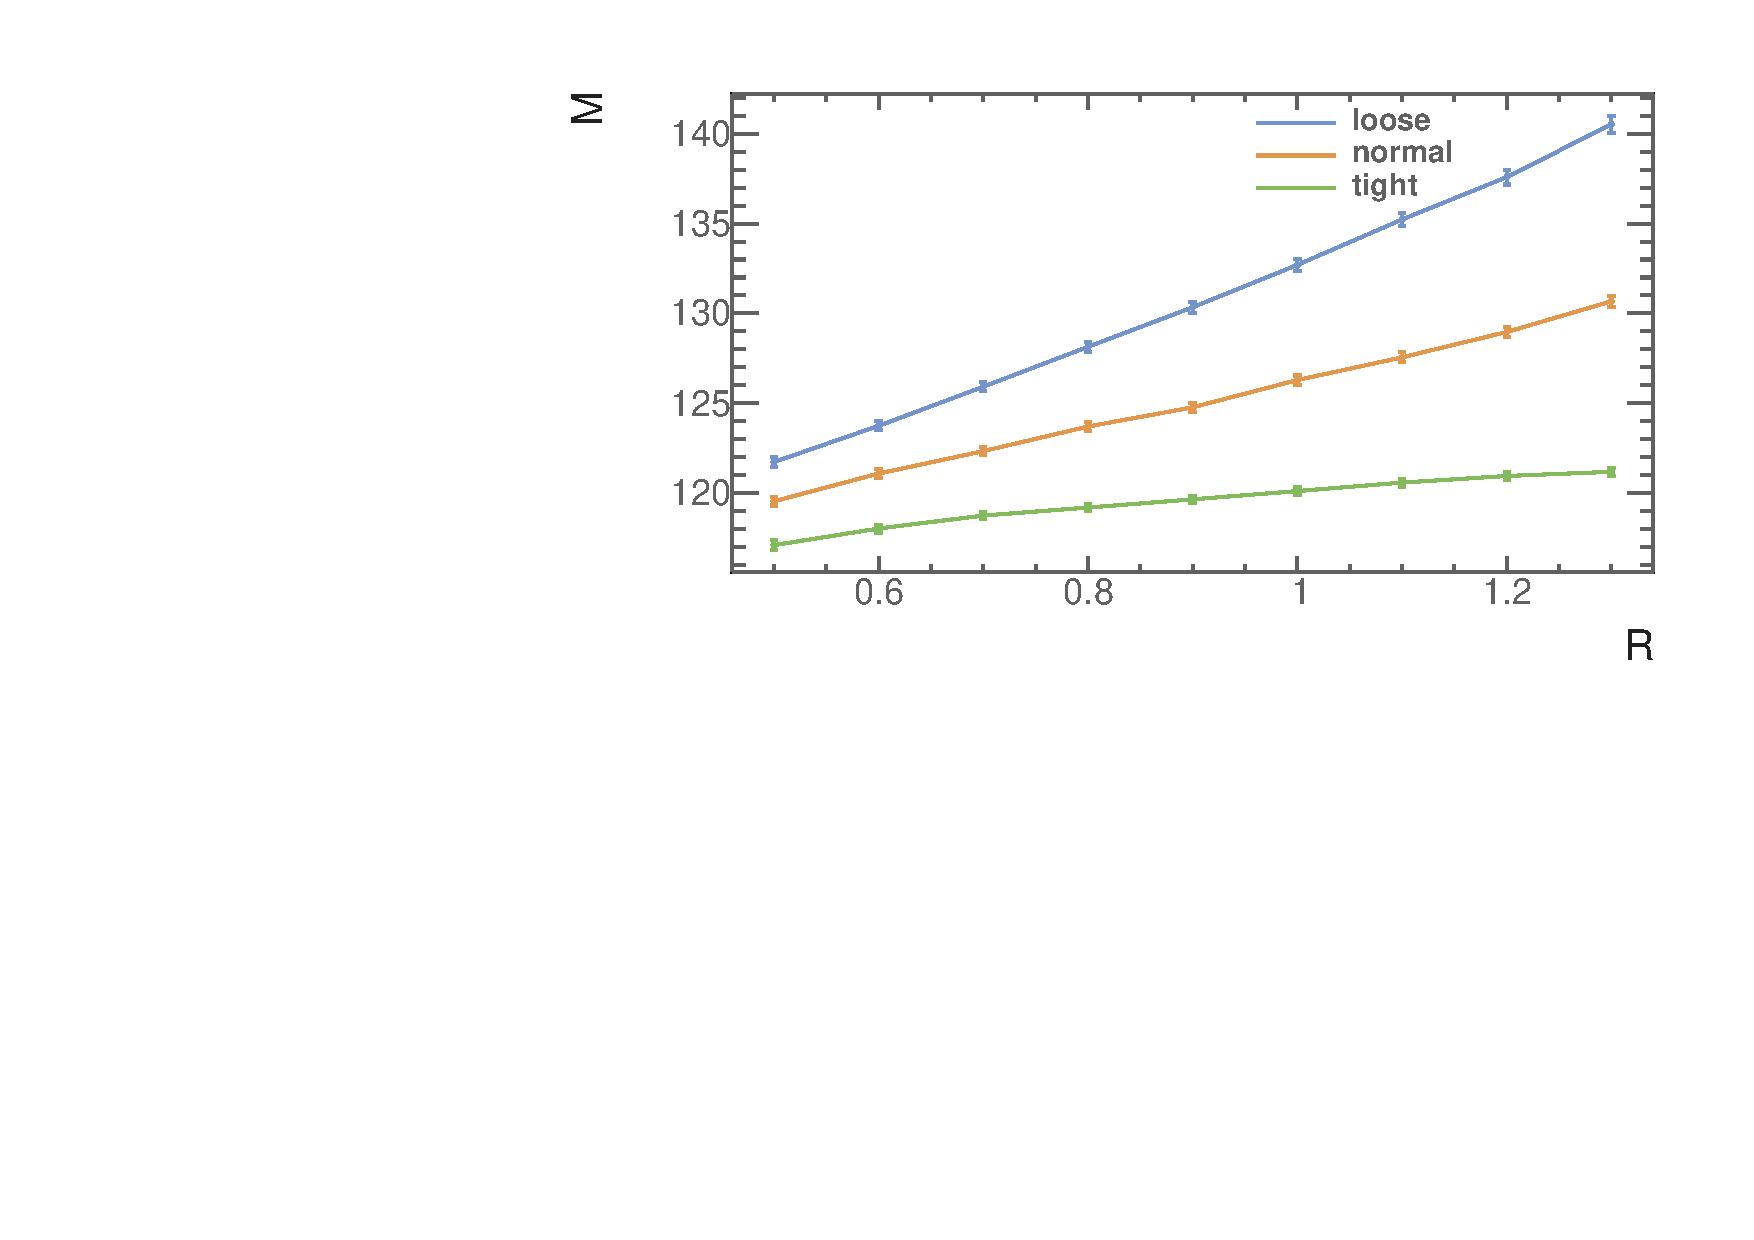
\includegraphics[width=\textwidth]{{doubleHiggs/resolution/ILD_1.4TeV_Higgs1_M_R}.pdf}
    \caption{}
    \label{fig:doubleHiggs1.4Higgs1M}
  \end{subfigure}
  \begin{subfigure}[b]{0.45\textwidth}
    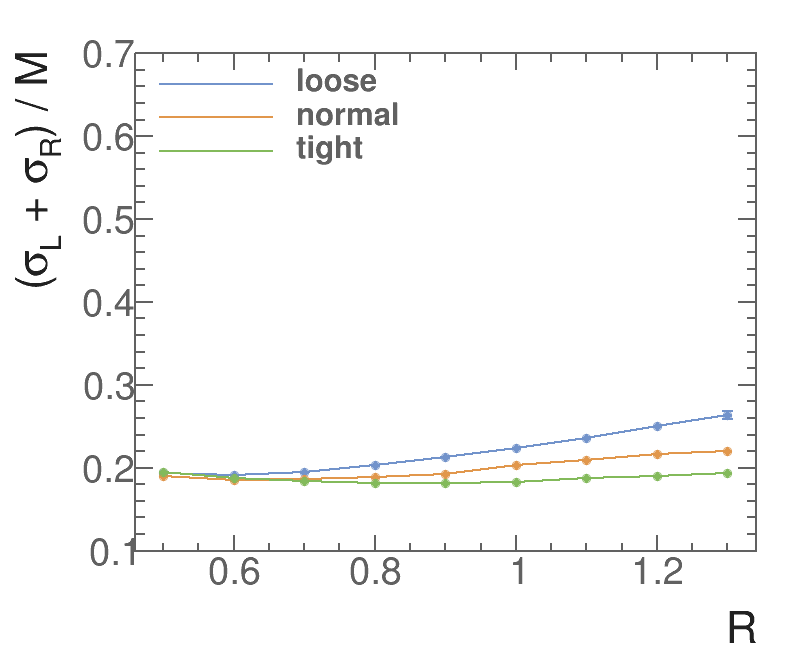
\includegraphics[width=\textwidth]{{doubleHiggs/resolution/ILD_1.4TeV_Higgs1_SigmaL_add_SigmaR_divide_M_testR}.pdf}
    \caption{}
    \label{fig:doubleHiggs1.4Higgs1Sigma}
  \end{subfigure}
  \begin{subfigure}[b]{0.45\textwidth}
    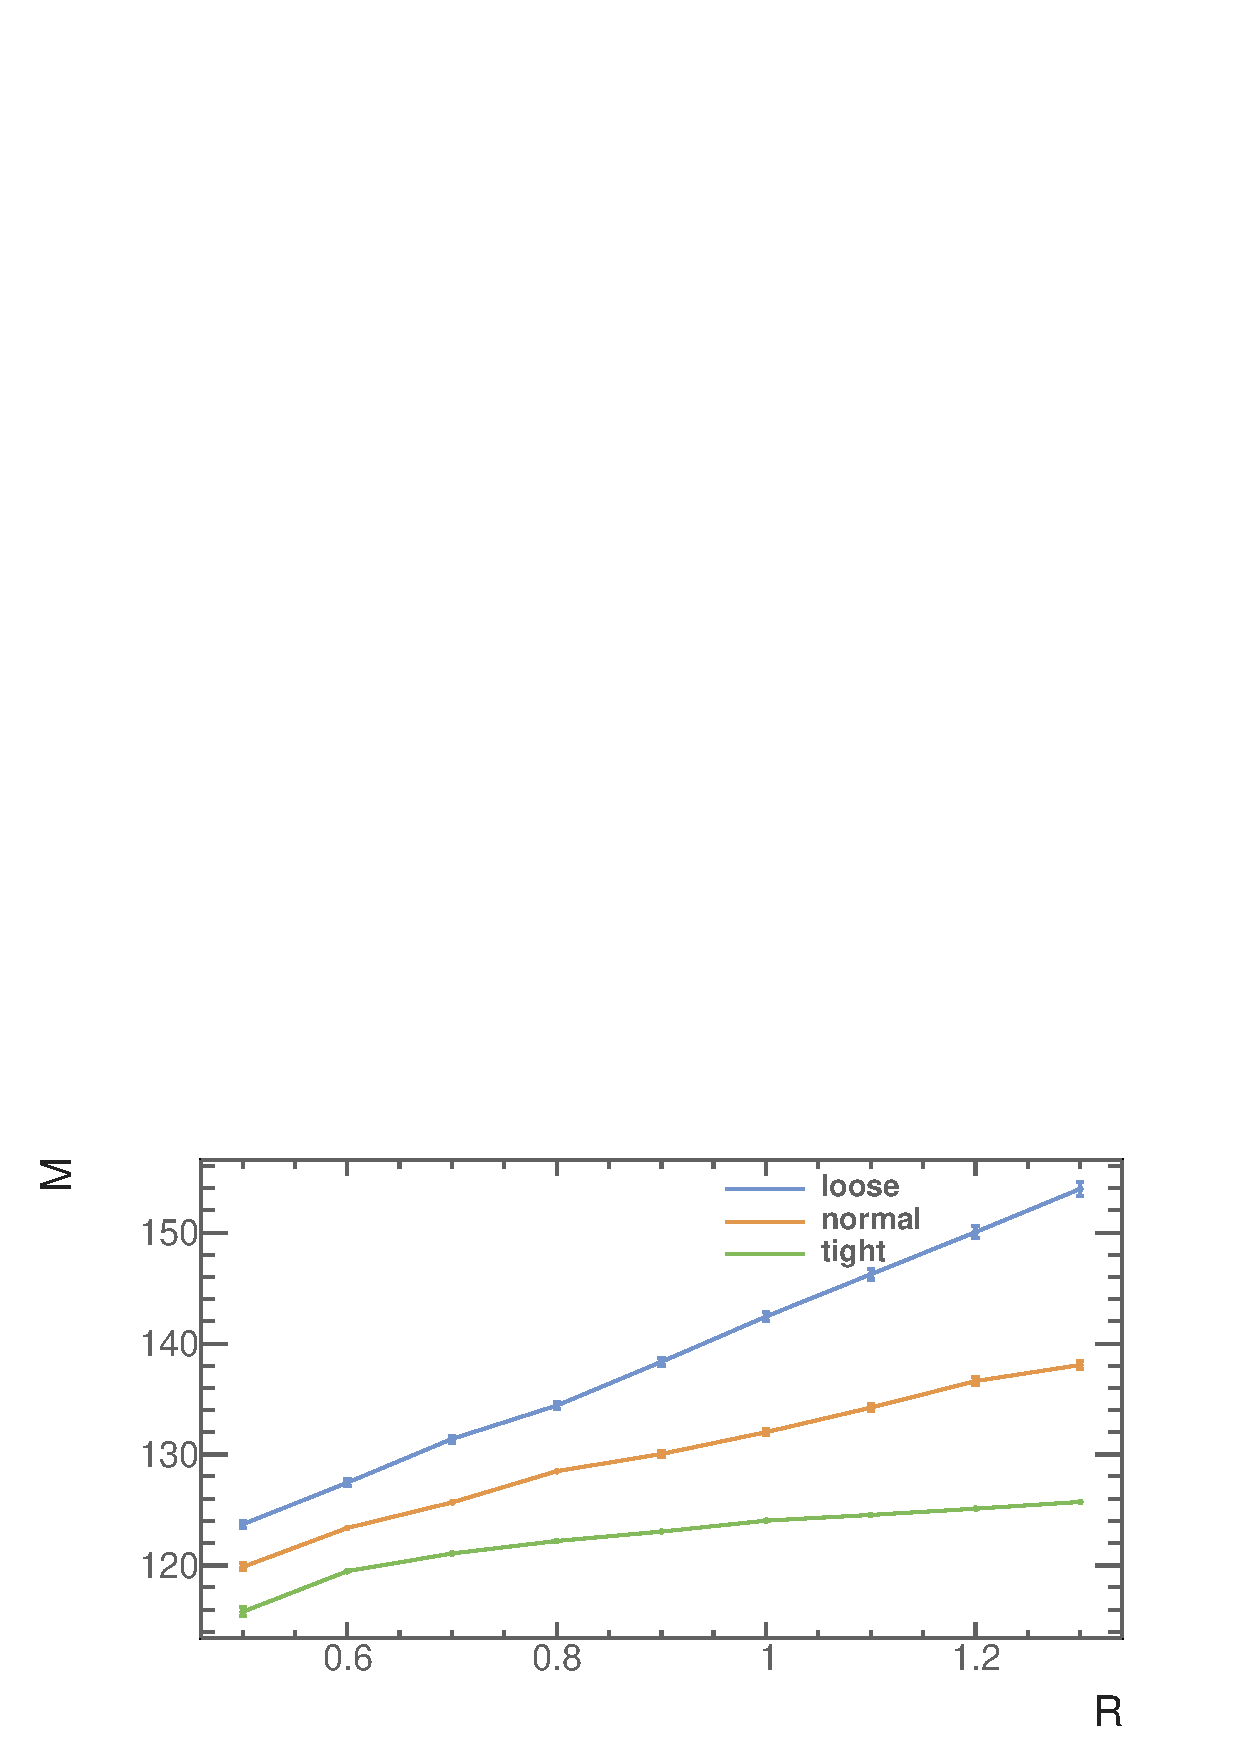
\includegraphics[width=\textwidth]{{doubleHiggs/resolution/ILD_1.4TeV_Higgs2_M_R}.pdf}
    \caption{}
    \label{fig:doubleHiggs1.4Higgs2M}
  \end{subfigure}
  \begin{subfigure}[b]{0.45\textwidth}
    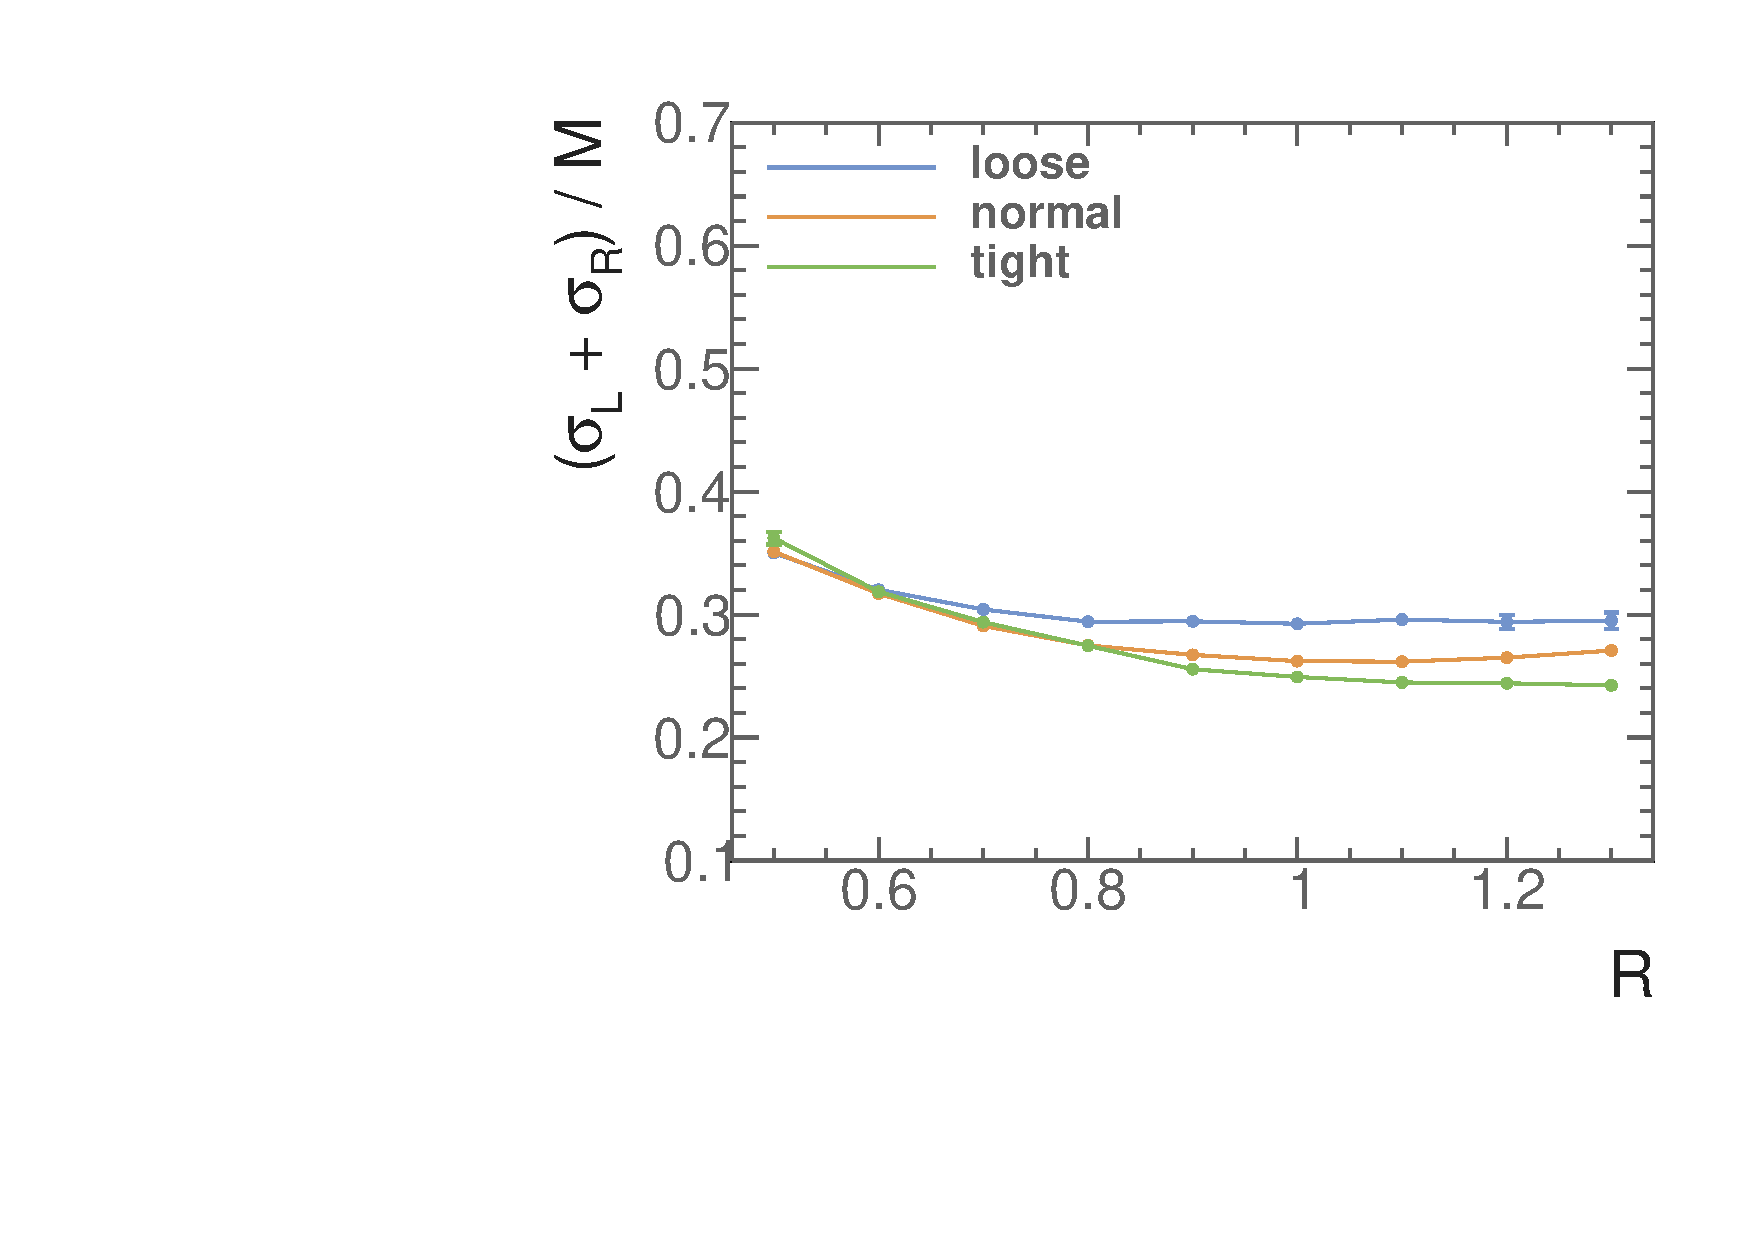
\includegraphics[width=\textwidth]{{doubleHiggs/resolution/ILD_1.4TeV_Higgs2_SigmaL_add_SigmaR_divide_M_testR}.pdf}
    \caption{}
    \label{fig:doubleHiggs1.4Higgs2Sigma}
  \end{subfigure}
  \begin{subfigure}[b]{0.45\textwidth}
    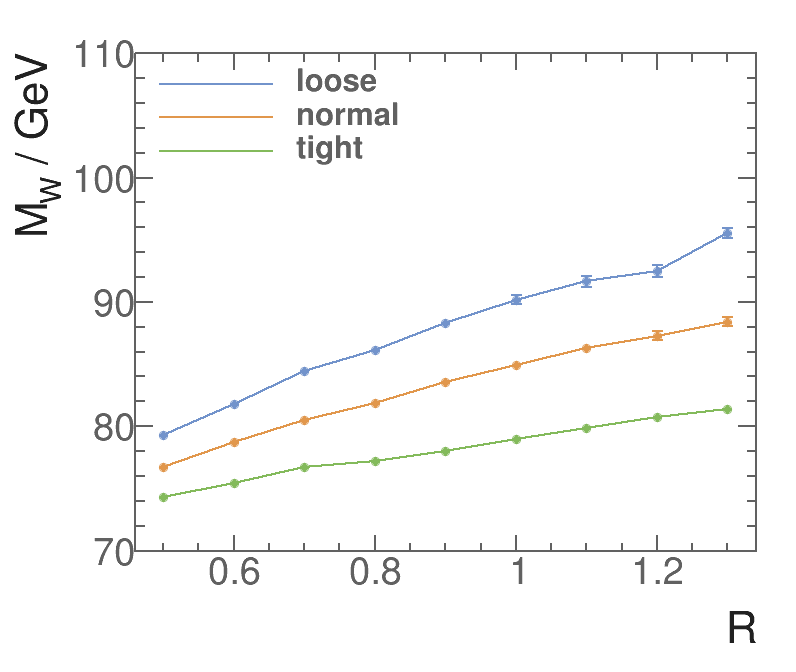
\includegraphics[width=\textwidth]{{doubleHiggs/resolution/ILD_1.4TeV_W_M_testR}.pdf}
    \caption{}
    \label{fig:doubleHiggs1.4WM}
  \end{subfigure}
  \begin{subfigure}[b]{0.45\textwidth}
    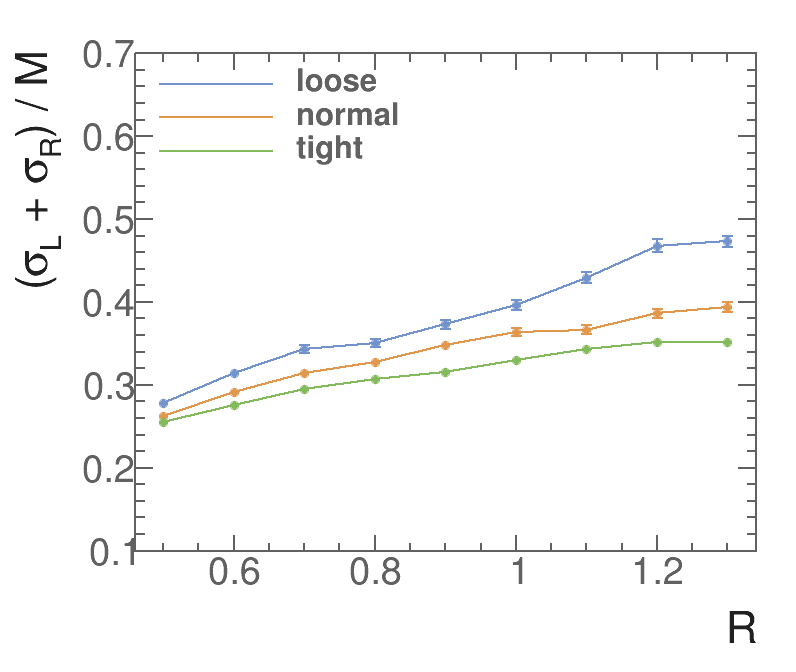
\includegraphics[width=\textwidth]{{doubleHiggs/resolution/ILD_1.4TeV_W_SigmaL_add_SigmaR_divide_M_testR}.pdf}
    \caption{}
    \label{fig:doubleHiggs1.4WSigma}
  \end{subfigure}
\caption[Fitted mass, and resolution of \Hbb, \HWW and \PW at \rootS{1.4}]%
   {Distributions of: a) fitted mass peak positions for \Hbb; b) relative mass peak widths for \Hbb; c) fitted mass peak positions for \HWW;  d) relative mass peak widths for \HWW; e) fitted mass peak positions for \PW; and f) relative mass peak widths for \PW. All plots show the variation of the fitted masses and mass resolutions as a function of $R$ for  loose, normal, and tight selected \PFO collections at \rootS{1.4}, using \eeToHHbbWWHad samples.}
   \label{fig:doubleHiggs1.4TeVMassFit}
\end{figure}

\begin{table}[!htbp]
\begin{tabular}{lrr}
\hline
\hline
Fitted jet parameter  &  \rootS{1.4}   &  \rootS{3}  \\
\hline
$\mu_{\Hbb}$ & $122.3_{\pm0.2}$  & $119.1_{\pm0.3}$  \\
$\sigma_{L,\Hbb}$ & $15.2_{\pm0.2}$  & $15.0_{\pm0.3}$  \\
$\sigma_{R,\Hbb}$ & $7.6_{\pm0.2}$ & $8.4_{\pm0.2}$  \\
\hline
$\mu_{\HWW}$ & $125.7_{\pm0.2}$  & $123.0_{\pm0.3}$  \\
$\sigma_{L,\HWW}$ & $29.4_{\pm0.3}$  & $36.6_{\pm0.6}$  \\
$\sigma_{R,\HWW}$ & $7.2_{\pm0.2}$ & $7.4_{\pm0.2}$  \\
\hline
$\mu_{\PW}$ & $80.5_{\pm0.2}$ & $78.1_{\pm0.3}$ \\
$\sigma_{L,\PW}$ & $16.2_{\pm0.3}$ & $13.1_{\pm0.4}$  \\
$\sigma_{R,\PW}$ & $9.0_{\pm0.2}$  &  $9.5_{\pm0.2}$  \\
\hline
\hline
\end{tabular}
\caption
[The fitted mass parameters of optimal jet reconstruction at \rootS{1.4}] %
{The fitted mass  parameters for  \rootS{1.4}  analysis: $R = 0.7$ using the \normalPFO, and for  \rootS{3} analysis: $R = 0.7$ using the \tightPFO.}
\label{tab:doubleHiggsFitParameters}
\end{table}

A separate jet reconstruction optimisation is performed for \rootS{3} analysis. \FIGURE{fig:doubleHiggs3TeVMassFit} shows the variation of fitted mass peak positions and  the relative mass resolutions for \Hbb, \HWW, and \PW as function of $R$ and \PFO collections. The relative mass resolution of \PW boson quickly degrades with an increasing $R$. The fitted mass peak positions also increases more rapidly with the increase of $R$, compared with the fitted mass peak positions at \rootS{1.4}. This is because at a higher centre-of-mass energy, more beam induced background particles are produced. The background particles, if included in the jets, will increase the invariant masses of the fitted physical bosons. Based on this study,  $R = 0.7$  with the \tightPFO was chosen for the \rootS{3} analysis. With chosen parameters, the better relative mass resolutions compensate for the invariant masses being slightly smaller than simulated values. The extracted fitted parameters of optimal jet reconstructions at \rootS{3} are summarised in \Table{tab:doubleHiggsFitParameters}.


%This choice  gives good fitted mass peak positions for \Hbb, \HWW and \PW. The extracted fitted parameters of optimal jet reconstructions are summarised in \Table{tab:doubleHiggsFitParameters}.
%The relative mass resolution of \PW worsen with increasing $R$, hence optimal choice favours a small $R$ and \tightPFO. The optimal jet reconstruction parameters is  \tightPFO with $R = 0.7$. The excellent mass resolution with the optimal choice compensates for the invariant masses being slightly smaller than simulated values. The fitted mass peak positions and mass resolutions  1of the chosen jet reconstruction are listed in \Table{tab:doubleHiggs3TeVFitParameters}


\begin{figure}[!htbp]
  \begin{subfigure}[b]{0.45\textwidth}
    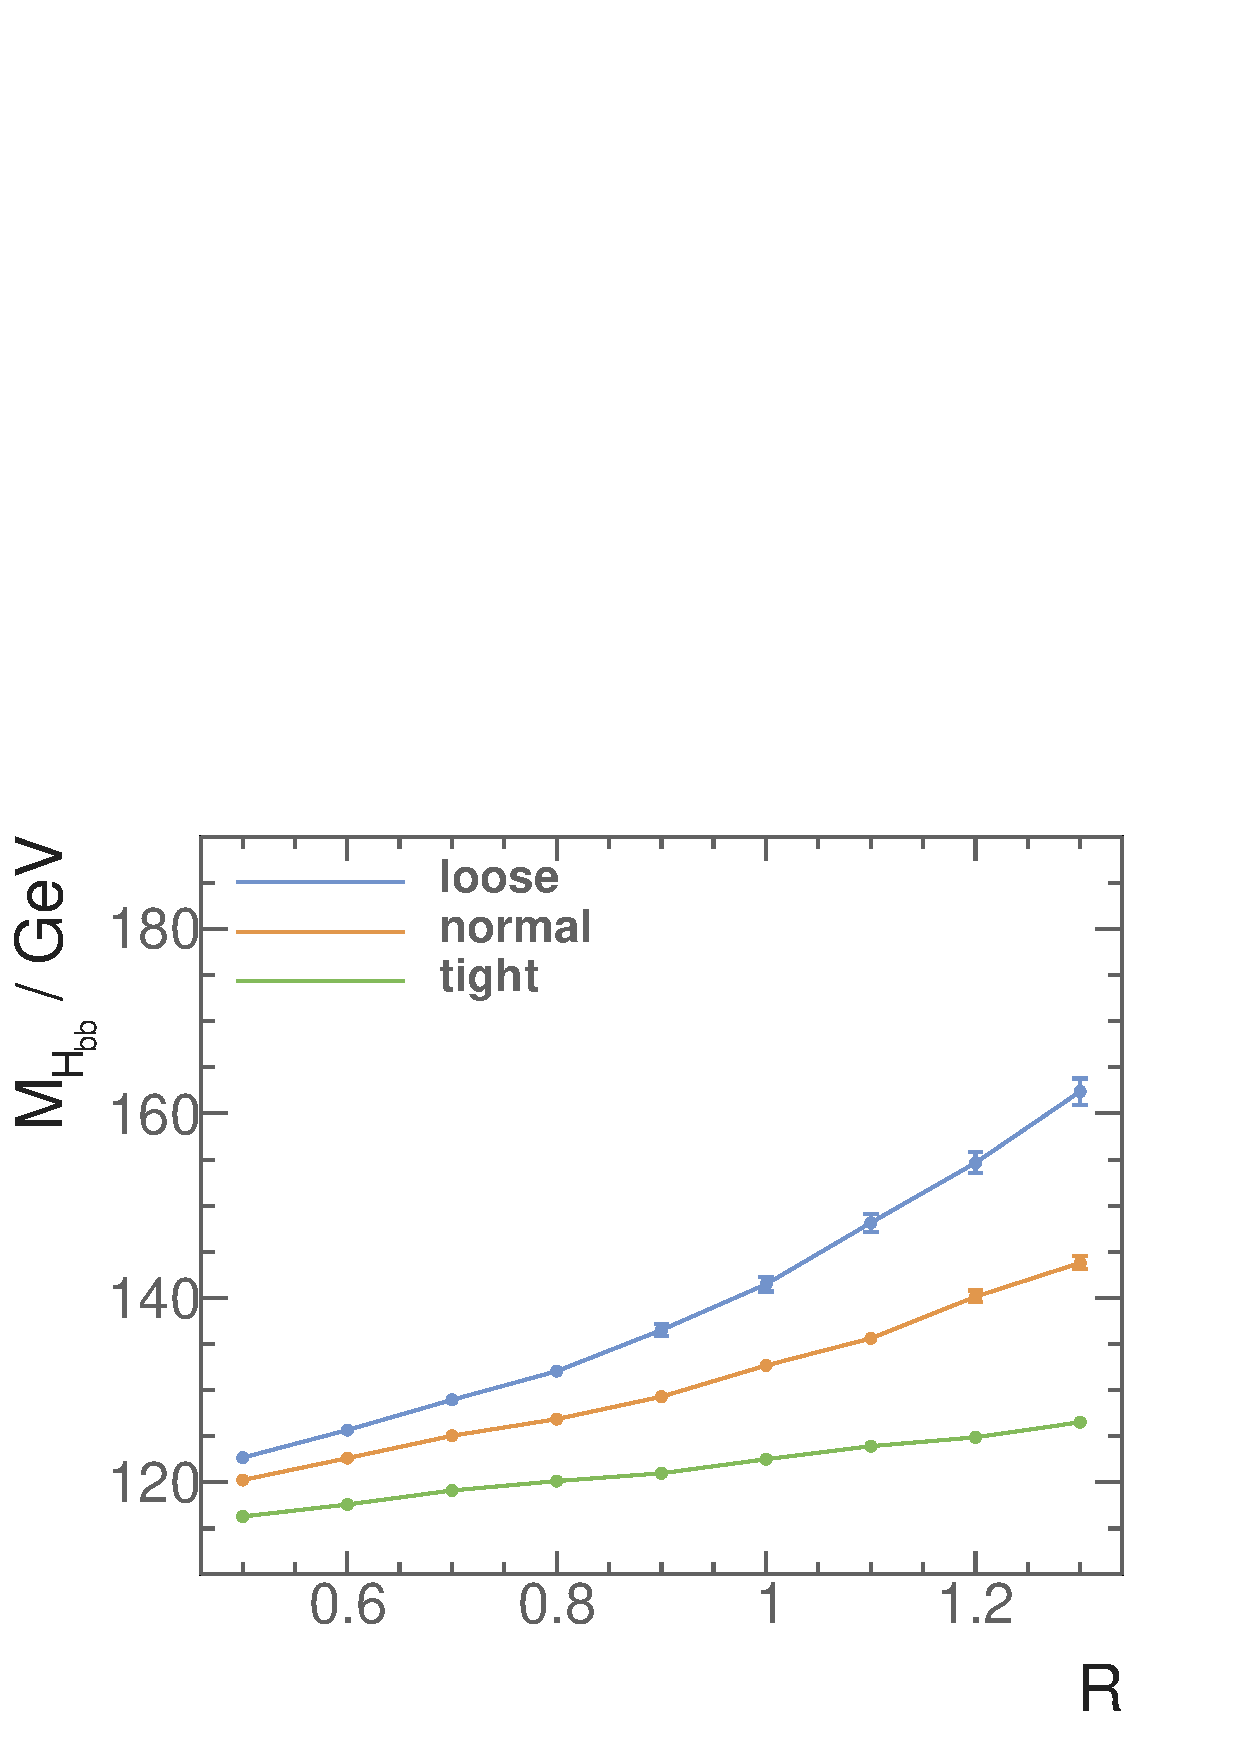
\includegraphics[width=\textwidth]{{doubleHiggs/resolution/ILD_3TeV_Higgs1_M_R}.pdf}
    \caption{}
    \label{fig:doubleHiggs3Higgs1M}
  \end{subfigure}
  \begin{subfigure}[b]{0.45\textwidth}
    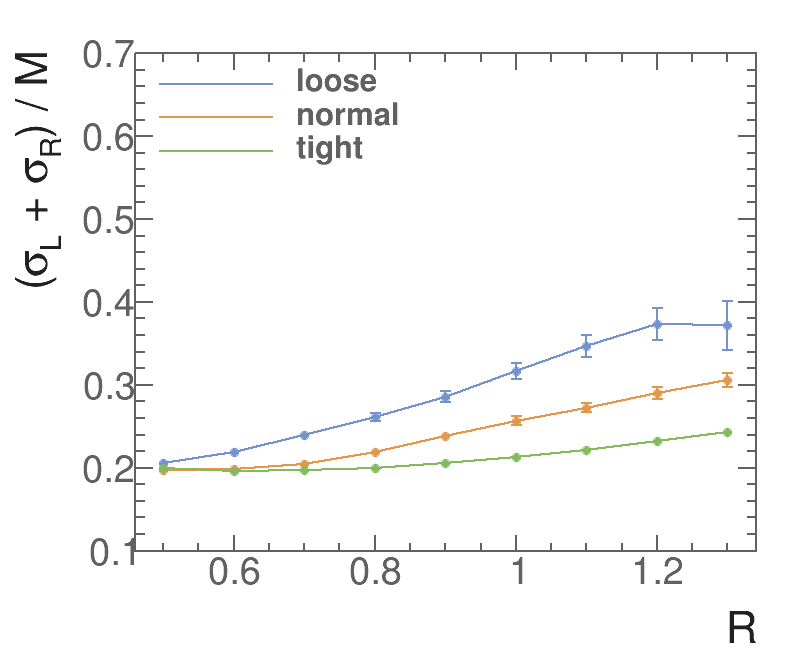
\includegraphics[width=\textwidth]{{doubleHiggs/resolution/ILD_3TeV_Higgs1_SigmaL_add_SigmaR_divide_M_testR}.pdf}
    \caption{}
    \label{fig:doubleHiggs3Higgs1Sigma}
  \end{subfigure}
  \begin{subfigure}[b]{0.45\textwidth}
    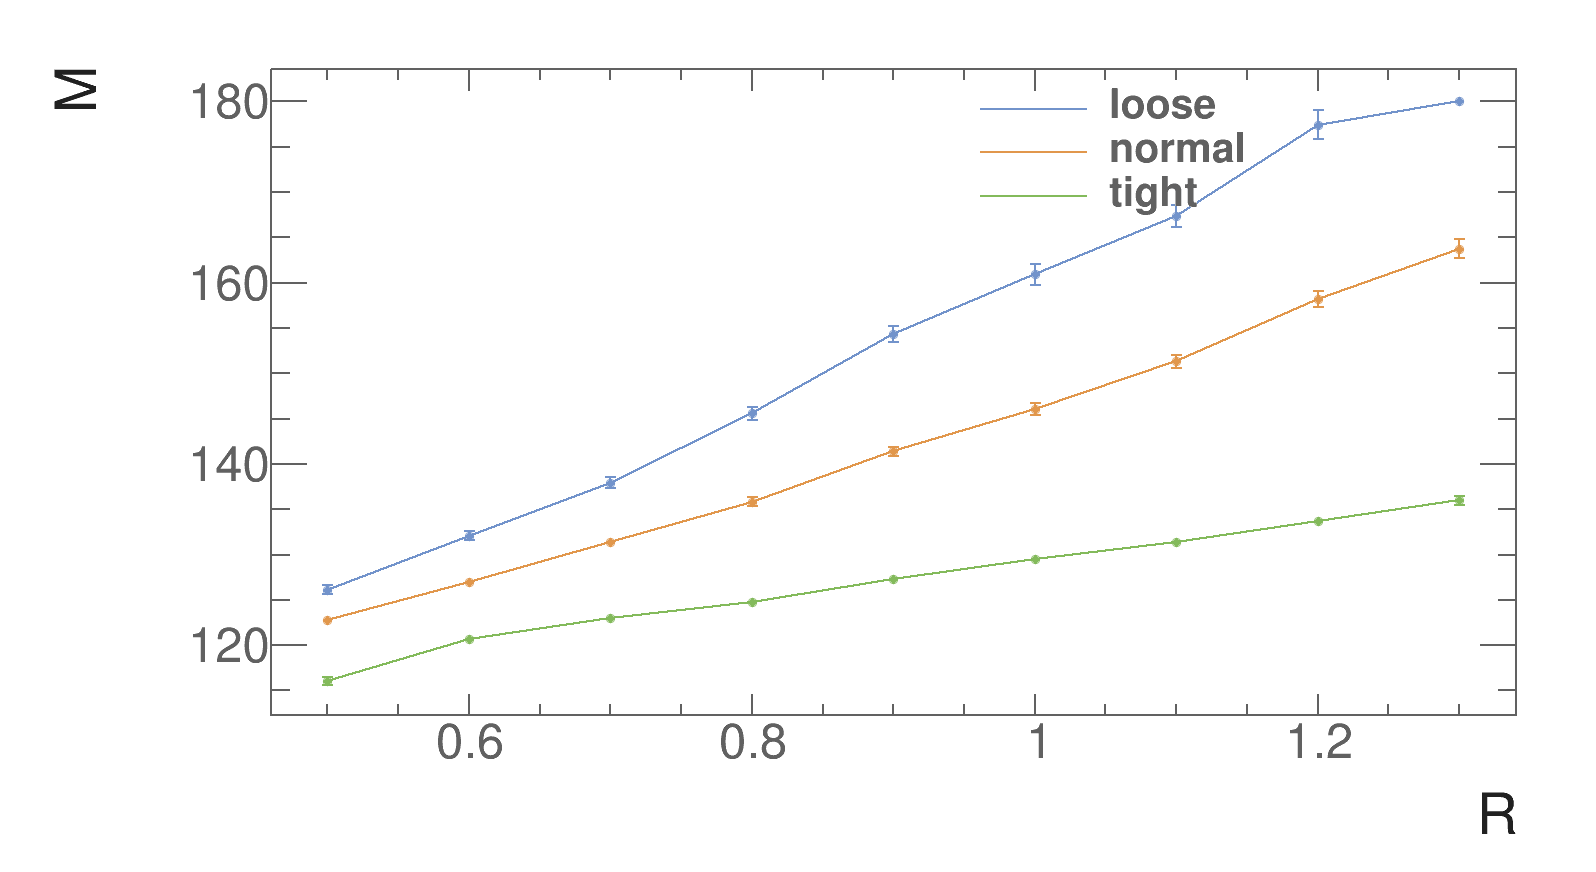
\includegraphics[width=\textwidth]{{doubleHiggs/resolution/ILD_3TeV_Higgs2_M_R}.pdf}
    \caption{}
    \label{fig:doubleHiggs3Higgs2M}
  \end{subfigure}
  \begin{subfigure}[b]{0.45\textwidth}
    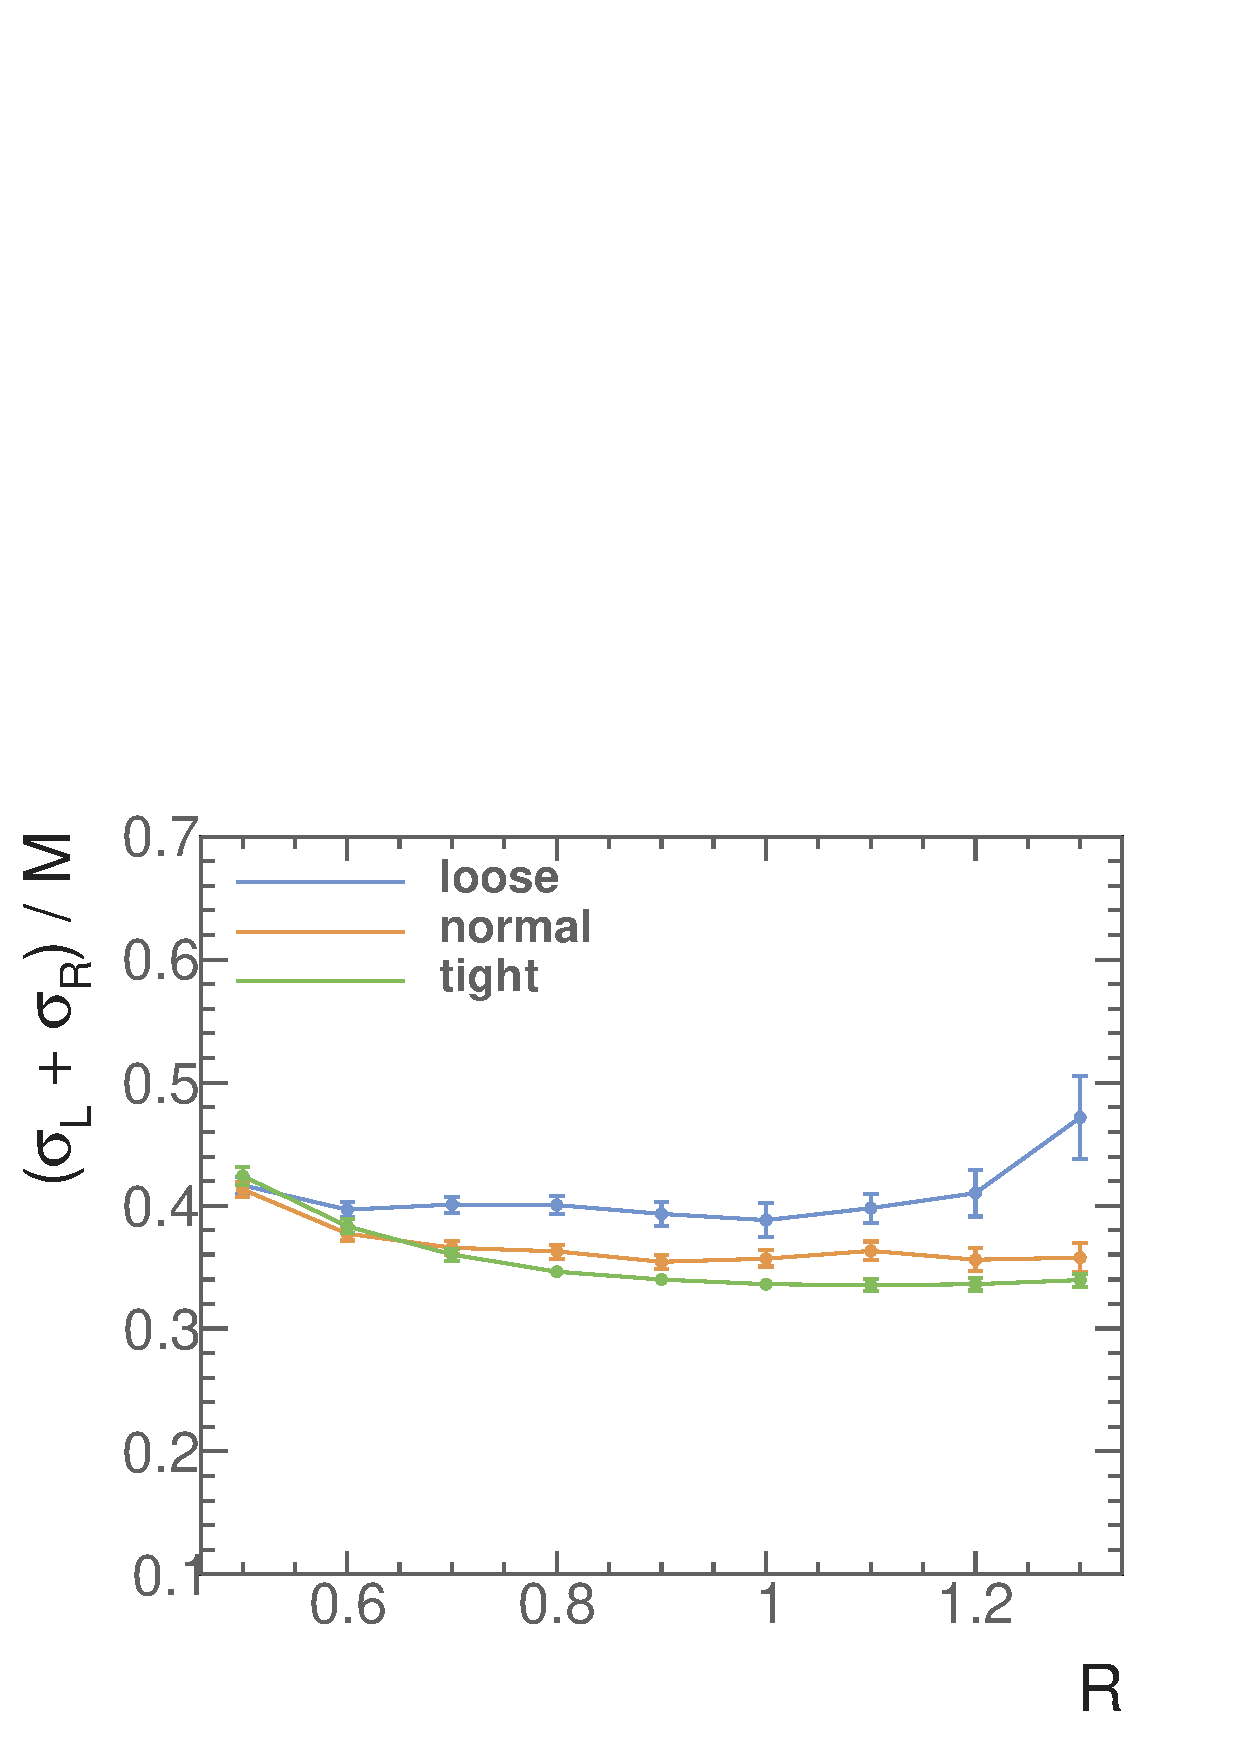
\includegraphics[width=\textwidth]{{doubleHiggs/resolution/ILD_3TeV_Higgs2_SigmaL_add_SigmaR_divide_M_testR}.pdf}
    \caption{}
    \label{fig:doubleHiggs3Higgs2Sigma}
  \end{subfigure}
  \begin{subfigure}[b]{0.45\textwidth}
    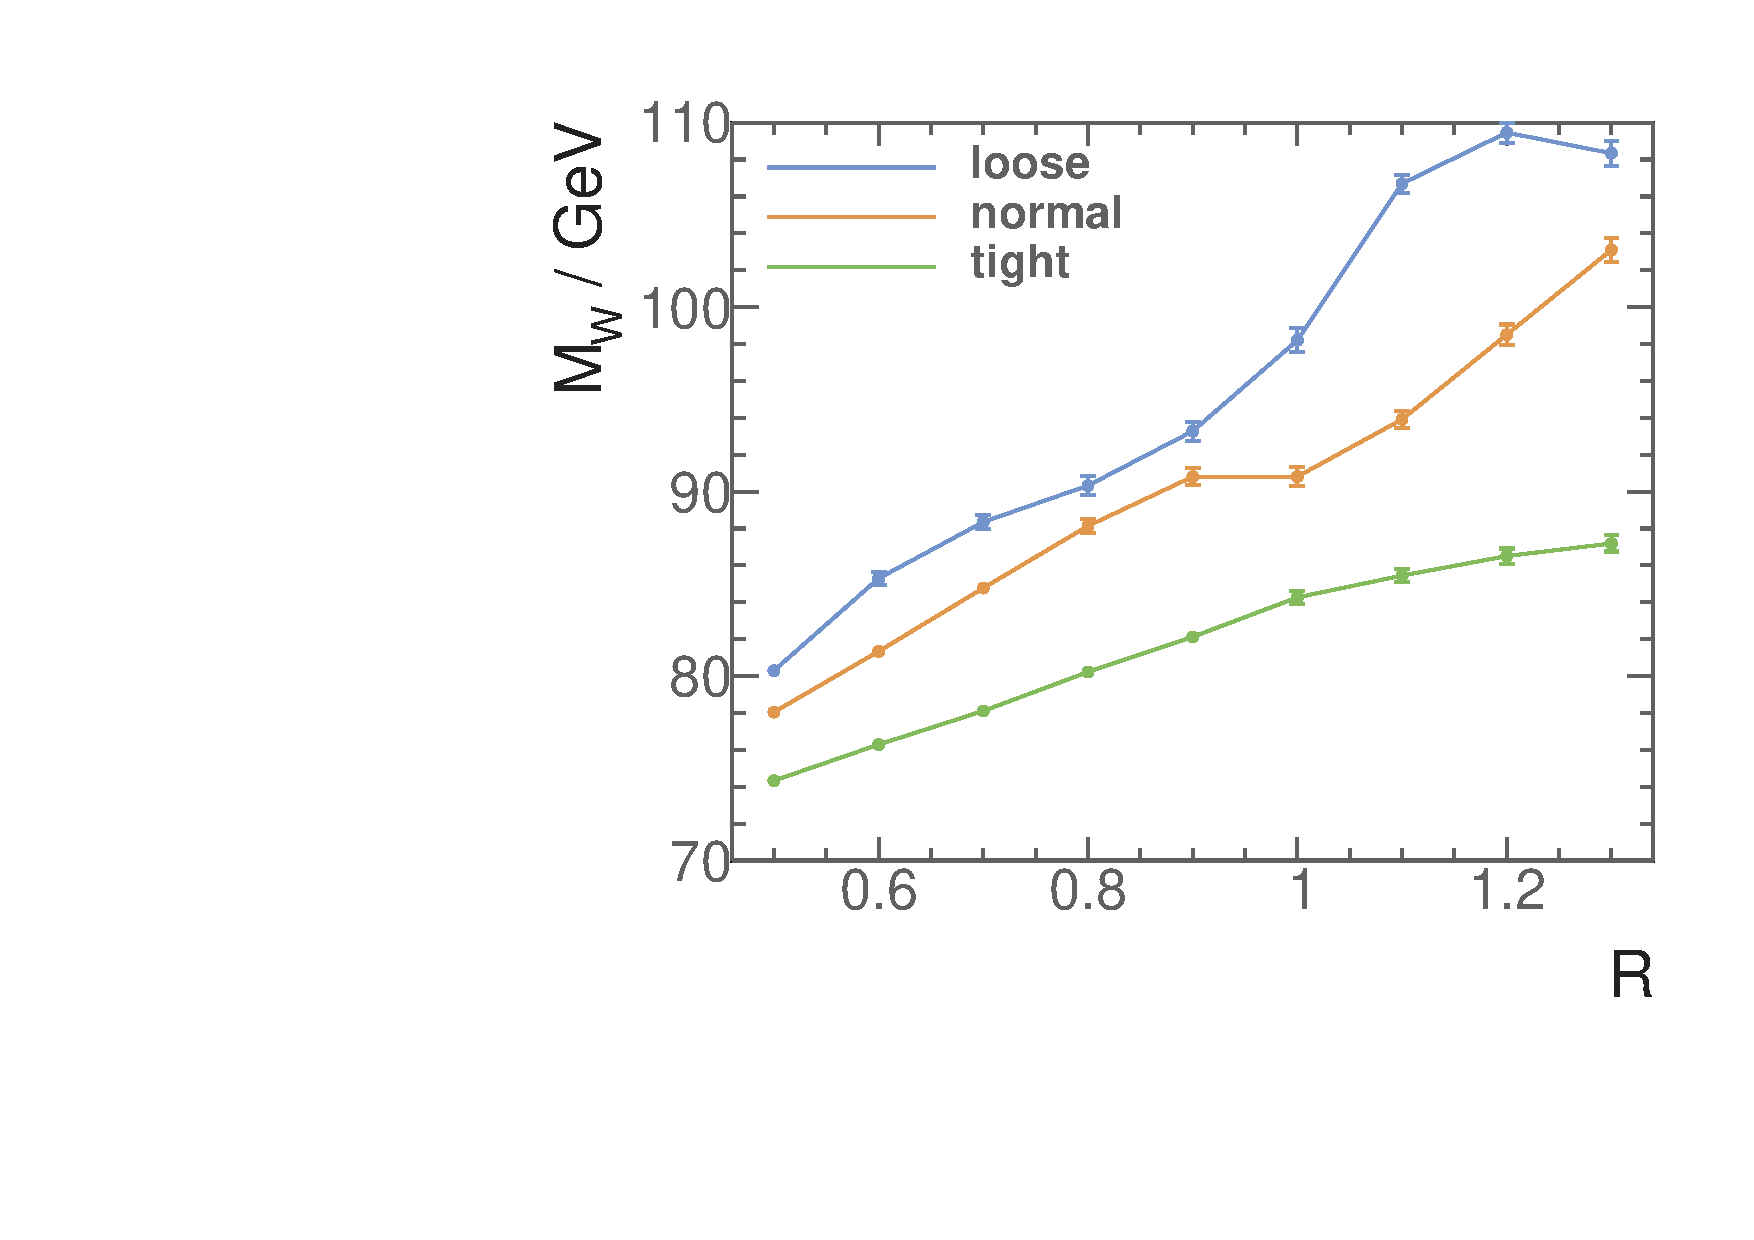
\includegraphics[width=\textwidth]{{doubleHiggs/resolution/ILD_3TeV_W_M_testR}.pdf}
    \caption{}
    \label{fig:doubleHiggs3WM}
  \end{subfigure}
  \begin{subfigure}[b]{0.45\textwidth}
    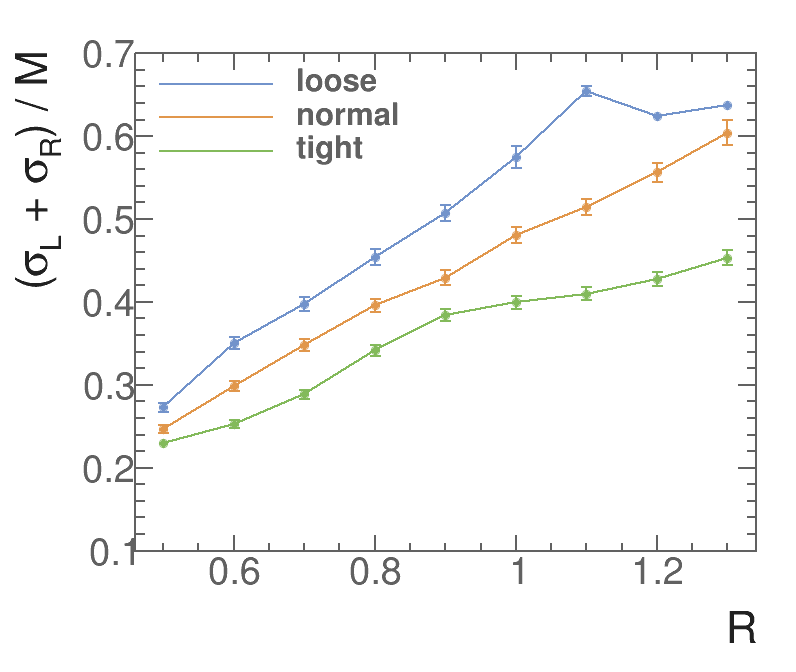
\includegraphics[width=\textwidth]{{doubleHiggs/resolution/ILD_3TeV_W_SigmaL_add_SigmaR_divide_M_testR}.pdf}
    \caption{}
    \label{fig:doubleHiggs3WSigma}
  \end{subfigure}
\caption[Fitted mass peak positions and relative mass resolution of \Hbb, \HWW and \PW at \rootS{3}.]%
{Distributions of: a) fitted mass peak positions of \Hbb; b) relative mass peak widths of \Hbb; c) fitted mass peak positions of \HWW; d) relative mass peak widths of \HWW; e) fitted mass peak positions of \PW; and f) relative mass peak widths of \PW. All plots show the variation of fitted masses and mass resolutions as a function of $R$ for loose, normal, and tight selected \PFO collections at \rootS{3}, using \eeToHHbbWWHad samples.}
   \label{fig:doubleHiggs3TeVMassFit}
\end{figure}

\section{Jet flavour tagging}
\label{sec:doubleHiggsFlavourTagging}

As the signal process, \eeToHHbbWWHad,  contains two \Pbottom quarks in the final state, identifying jets originated from \Pbottom quarks is an important part of the event selection.

%Pbottom jet (b-jet tag value), \lcfiplus \cite{Suehara:2015ura} software package is used.

%Another useful analysis technique is to identify jets from \Pbottom and \Pcharm quarks. These jets have signatory topologies. A combination of vertex finding and multivariate analysis is used to identify \Pbottom and \Pcharm jets.

The flavour tagging processor, \lcfiplus \cite{Suehara:2015ura} is used. The processor is based on the \textsc{LcfiVertex} package \cite{Bailey:2009ui}, which was used in the simulation studies for the \ILCloi \cite{Abe:2010aa,Aihara:2009ad} and the \CLICcdr \cite{Linssen:2012hp}.
%\lcfiplus is modular and can be used in any order. However here it will be described in the order that is used in this analysis.

%The current software is built for a future \ee collider.
After the previous jet clustering step, particles which are not in the beam jet are used as inputs for the flavour tagging. The flavour tagging algorithm identifies vertices, then re-cluster particles into jets. Lastly, the algorithm decides if a jet is a \Pbottom-quark jet or a \Pcharm-quark jet.


The vertex finding algorithms perform vertex fitting and identify primary and secondary vertices. There are two vertex refining algorithm. First algorithm rejects the topology of a  neutral particle that decays into pairs of charged particles, which can be mistaken as  the decay of \Pbottom or \Pcharm quarks. The second algorithm is performed after the re-clustering step to reconstruct more secondary vertices, with additional information from the jet clustering.

The jet re-clustering algorithm is a modified Durham algorithm, with additional constraint of the secondary vertices and the muons, which are identified from semi-leptonic decay of the quarks, falling into the same  jet as the quarks. This ensures the topology of the jet remains consistent with the hadronic decays of heavy quarks.


Having obtained re-clustered jets, the next step is the flavour tagging, which uses a multivariate classifier to determine if a jet is from \Pbottom quark or \Pcharm quark. \lcfiplus uses the Boosted Decision Tree MVA \multiclass classifier as implemented in the \TMVA software package \cite{Hocker:2007ht}. There are four categories for classification:  jets with zero, one, two properly reconstructed vertices, or a single-track pseudo-vertex. A jet can be classified into one of three classes: \Pbottom jet, \Pcharm jet, or a light flavour quark (\Pup, \Pdown or \Pstrange) jet.

The MVA \multiclass classifier was trained with \HepProcess{\Pep \Pem \to \PZ \APnu \Pnu} event at \rootS{1.4}, where \PZ decays to \HepProcess{\Pbottom\APbottom}, \HepProcess{\Pcharm\APcharm}, or \HepProcess{\Pup\APup/\Pdown\APdown/\Pstrange\APstrange}. The training sample contains missing momentum, which is similar to the signal sample. The training sample only has two quarks in the final states, which reduces the error in jet clustering and provides a good ground truth for training. The MVA classicisation efficiency with the training samples is shown in \Figure{fig:doubleHiggs1.4Btag}.

Having trained the MVA classifier, the MVA classifier is applied to the samples. Under the signal hypothesis, the re-clustering algorithm is set to find six jets. The normalised distribution of the highest b-jet tag value for the \eeToHHbbWWHad sample is shown in \Figure{fig:doubleHiggsBtagSignalPerformance}.

For the \rootS{3} analysis, the MVA classifier is re-trained with  \HepProcess{\Pep \Pem \to \PZ \APnu \Pnu} event at \rootS{3}. The performance of the flavour tagging  with training samples is shown in \Figure{fig:doubleHiggsBtag3TeV}. The performance at \rootS{3} is slightly worse than at \rootS{1.4}, because at the higher centre-of-mass energy, jets are more collimated and more difficult to separate.

%Compared to the performance at \rootS{1.4}, the performance is slightly worse, because at a high centre-of-mass energy, particles at more collimated and more difficult to separate. Therefore, the vertex identification and the flavour tagging performance are worse.



%The last step is to gather the information about vertices and jets, and deploy a multivariate analysis. The multivariate classier used, Boosted Decision Tree,  is implemented in the TMVA software package \cite{Hocker:2007ht}. A number of flavour sensitive variables are calculated. The jets are is divided into four subsets: jets with zero, one, two properly reconstructed vertices, or a single-track pseudo-vertex. For each subset, a jet can either be classified to a \Pbottom jet, a \Pcharm jet, or a light flavour quark jet (\Pup, \Pdown or \Pstrange). The multiclass classifier's response is normalised across different subsets.
%, and they will be referred in the subsequent physics analysis as the tag value.

%The samples for training the multiclass classifier are \HepProcess{\Pep \Pem \to \PZ \APnu \Pnu} at \rootS{1.4}, where \PZ decays to \HepProcess{\Pbottom\APbottom}, \HepProcess{\Pcharm\APcharm}, or \HepProcess{\Pup\APup/\Pdown\APdown/\Pstrange\APstrange}.

%The events to train the multiclass classifier are \HepProcess{\Pep \Pem \to \PZ \APnu \Pnu} event at \rootS{1.4}, where \PZ decays to \HepProcess{\Pbottom\APbottom}, \HepProcess{\Pcharm\APcharm}, or \HepProcess{\Pup\APup/\Pdown\APdown/\Pstrange\APstrange}. The selection efficiency of b jets and c jets with the training samples is shown in \Figure{fig:doubleHiggs1.4Btag}. The normalised distribution of the highest b-jet tag value for the signal events is shown in \Figure{fig:doubleHiggsBtagSignalPerformance}.

%To apply trained  multiclass classifier in the \lcfiplus processor, all the \PFOs in the initial reconstructed jet are fed into the processor. The jet re-clustering step in the \lcfiplus is set to find six jets. For each jet, values for the likelihood of a b-jet and a c-jet are obtained.
%At the training stage, the  jet re-clustering step is set to find two jets.  he outputs for a jet is three values, corresponding to the likelihood of the jet being a b-jet, a c-jet, or a light flavour quark jet.


%For the \rootS{3}, the flavour tagging processor is re-trained in the same way as in the \rootS{1.4} analysis. The training events are from the same channel but at \rootS{3}. The performance of the flavour tagging  with training samples is shown in \Figure{fig:doubleHiggsBtag3TeV}. Compared to the performance at \rootS{1.4}, the performance is slightly worse, because at a high centre-of-mass energy, particles at more collimated and more difficult to separate. Therefore, the vertex identification and the flavour tagging performance are worse.
%high energy or high energies?

\begin{figure}[!htbp]
 \begin{subfigure}[b]{0.45\textwidth}
    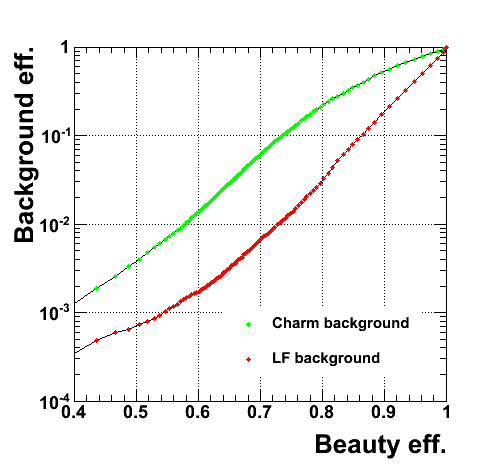
\includegraphics[width=\textwidth]{{doubleHiggs/eval-lcfiweights_R0_7_2jets-test}.pdf}
    \caption{\rootS{1.4}}
    \label{fig:doubleHiggs1.4Btag}
  \end{subfigure}
 \begin{subfigure}[b]{0.45\textwidth}
    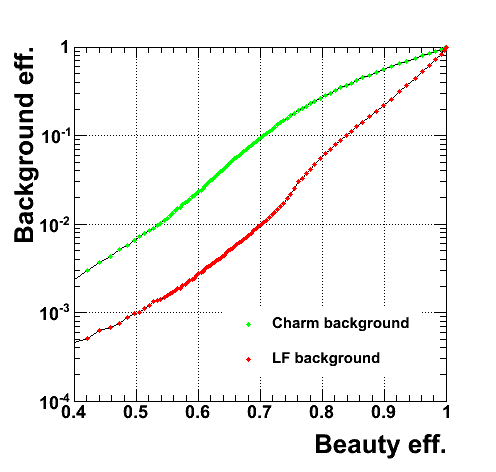
\includegraphics[width=\textwidth]{{doubleHiggs/eval-lcfiweights_tR0_7_3000_2jets-test}.pdf}
    \caption{\rootS{3}}
   \label{fig:doubleHiggsBtag3TeV}
  \end{subfigure}
\caption
   {Performance of b-jet tagging with \HepProcess{\Pep \Pem \to \PZ \APnu \Pnu} samples, where \PZ decays to \HepProcess{\Pbottom\APbottom}, \HepProcess{\Pcharm\APcharm}, or \HepProcess{\Pup\APup/\Pdown\APdown/\Pstrange\APstrange} at: a) \rootS{1.4}; and b) \rootS{3}.}
   \label{fig:doubleHiggsBtag}
\end{figure}


\begin{figure}[!htbp]
    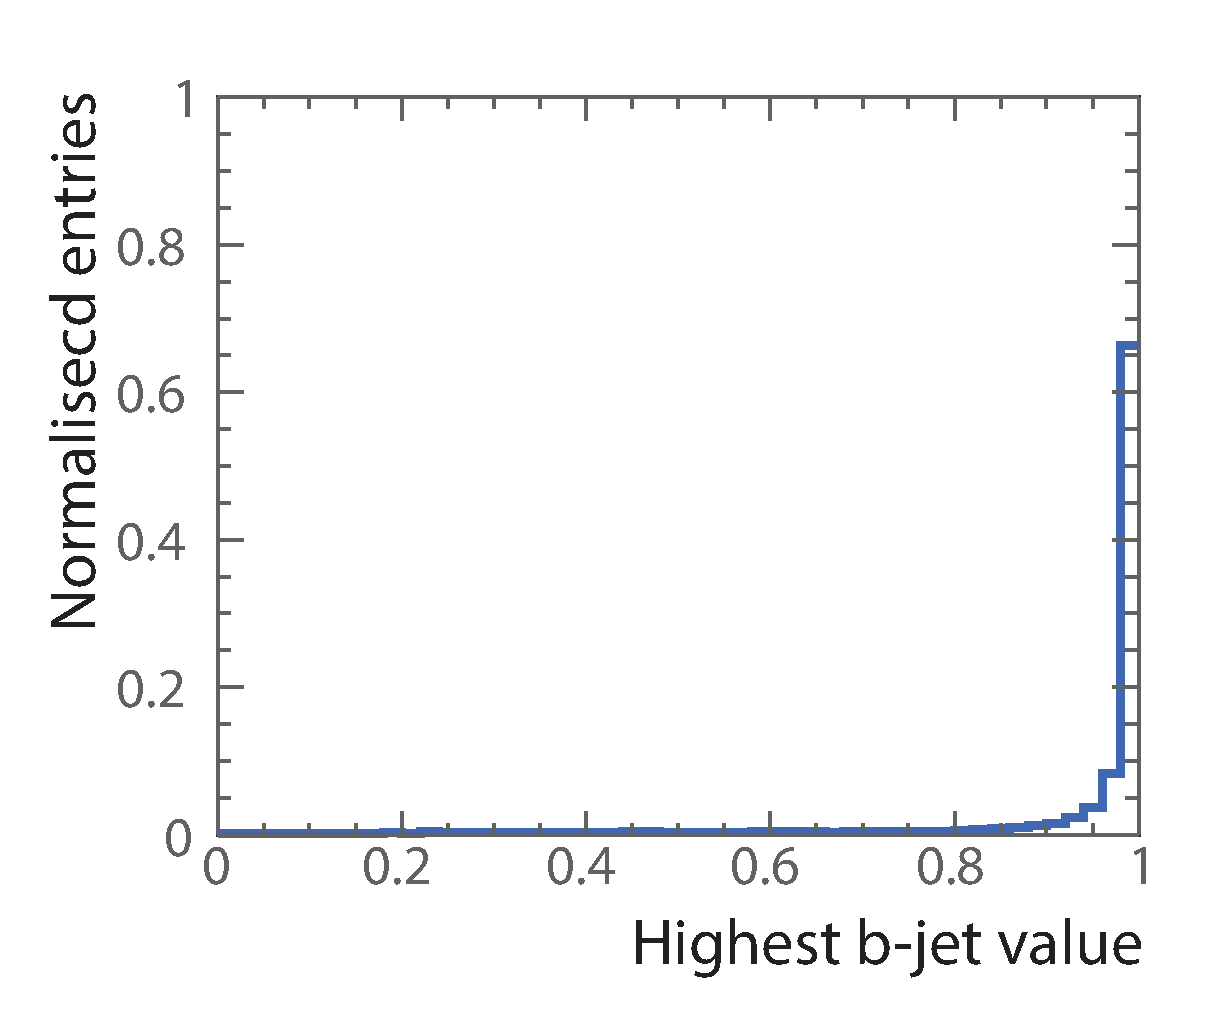
\includegraphics[width=0.45\textwidth]{{doubleHiggs/jetPairing/nR0_7_6jet_btag2_bTag1_TMVA20170223R0_7_qq_btag2_prepare2}}
\caption
   {The distribution of the highest b-jet value for the \eeToHHbbWWHad events  at \rootS{1.4}. The area under the curve is normalised to unity.}
   \label{fig:doubleHiggsBtagSignalPerformance}
\end{figure}
%The flavour tagging is performed after the initial jet reconstruction, and all the \PFOs in the reconstructed jets are input into the \lcfiplus flavour tagging processor. Therefore, the classifier in the \lcfiplus processor is trained for a specific \PFO collection and a specific jet reconstruction algorithm. The outputs of the processor for a jet are three values, corresponding to the likelihood of the jet being a \Pbottom jet, a \Pcharm jet, or a light flavour quark jet.

%The flavour tagging is performed after the initial jet reconstruction using optimal jet reconstruction parameters.  \PFOs in the reconstructed jets are the inputs to the flavour tagging processor. \lcfiplus processor includes a multiclass classifier which needs to be trained.


\subsection{Mutually exclusive cuts for \eeToHHbbWW and \eeToHHbbbb}
\label{sec:doubleHiggsMutualExclusive}

The two \eeToHH final states with the largest branching fractions are \eeToHHbbbb (31.5\%) and \eeToHHbbWW (25.9\%). These two final states have different topologies and are subjects of two analysis strategies. The \eeToHHbbWW final state is the subject of this thesis.  The study of the \eeToHHbbbb final state is the subject of an independent analysis. Because the results of the two studies are subsequently combined, a set of cuts are designed to separate  samples, for both signal and background events, into two mutually exclusive sets for  two independent analyses. This ensures there are no correlations between two analyses.

%This eases the difficulty of combining sub-channels as correlations between sub-channels need not to be considered where samples are mutually exclusive.
%With the jet clustering and b-jet tagging information,

The most distinctive difference between the \eeToHHbbWW and \eeToHHbbbb sub-channels is the different jet multiplicity  and the different number of b-jets in the final state. Consequently variables relating to the number of b-jets and total number of jets are suitable for separating the two sub-channels.

 \FIGURE{fig:doubleHiggsMutualPreselection} shows the sum of b-jet tag values, when the event is clustered into four jets, as a function of $-\log\parenths{\y{34}}$ for the hadronic \WW decay in \eeToHHbbWW and \eeToHHbbbb. As expected,  the two sub-channels can be clearly separated in this two dimensional phase space. A rectangular cut can be used to  separate the phase space into two spaces, donated as $S$ and $\neg{S}$. The hadronic \WW decay in \eeToHHbbWW events should  be contained in phase space $S$, and the \eeToHHbbbb events should be contained in phase space $\neg{S}$.

%To maximise the separation of two sub-channels, a set of cuts are found by maximising the product of the fraction of the sub-channel events in each space:
The optimal cuts are chosen such that they maximise:
\begin{equation}
\varepsilon = \frac{N_{\text{\eeToHHbbWW, hadronic}} \in S} {N_{\text{\eeToHHbbWW, hadronic}}} \times \frac{N_{\eeToHHbbbb} \in \neg{S}} {N_{\eeToHHbbbb}} ,
\end{equation}
where $N \in S$ indicates number of events in the phase space $S$.

Several combinations of pairs of variables were considered. In each case, the product of the fraction of the sub-channel events in each space, $\varepsilon$ was maximised. This procedure identified $\sumBtag{4} < 2.3, \,-\log\parenths{\y{34}} < 3.7$ as the best choice with 86\% of  the hadronic \WW decay in \eeToHHbbWW events are in $S$ and 78\% of the \eeToHHbbbb events are in $\neg{S}$. The full list of fraction of events after passing mutually exclusive cuts for individual background processes are listed in \Table{tab:doubleHiggs1.4TeVPreslection}.


\begin{figure}[!htbp]
  \begin{subfigure}[b]{0.45\textwidth}
    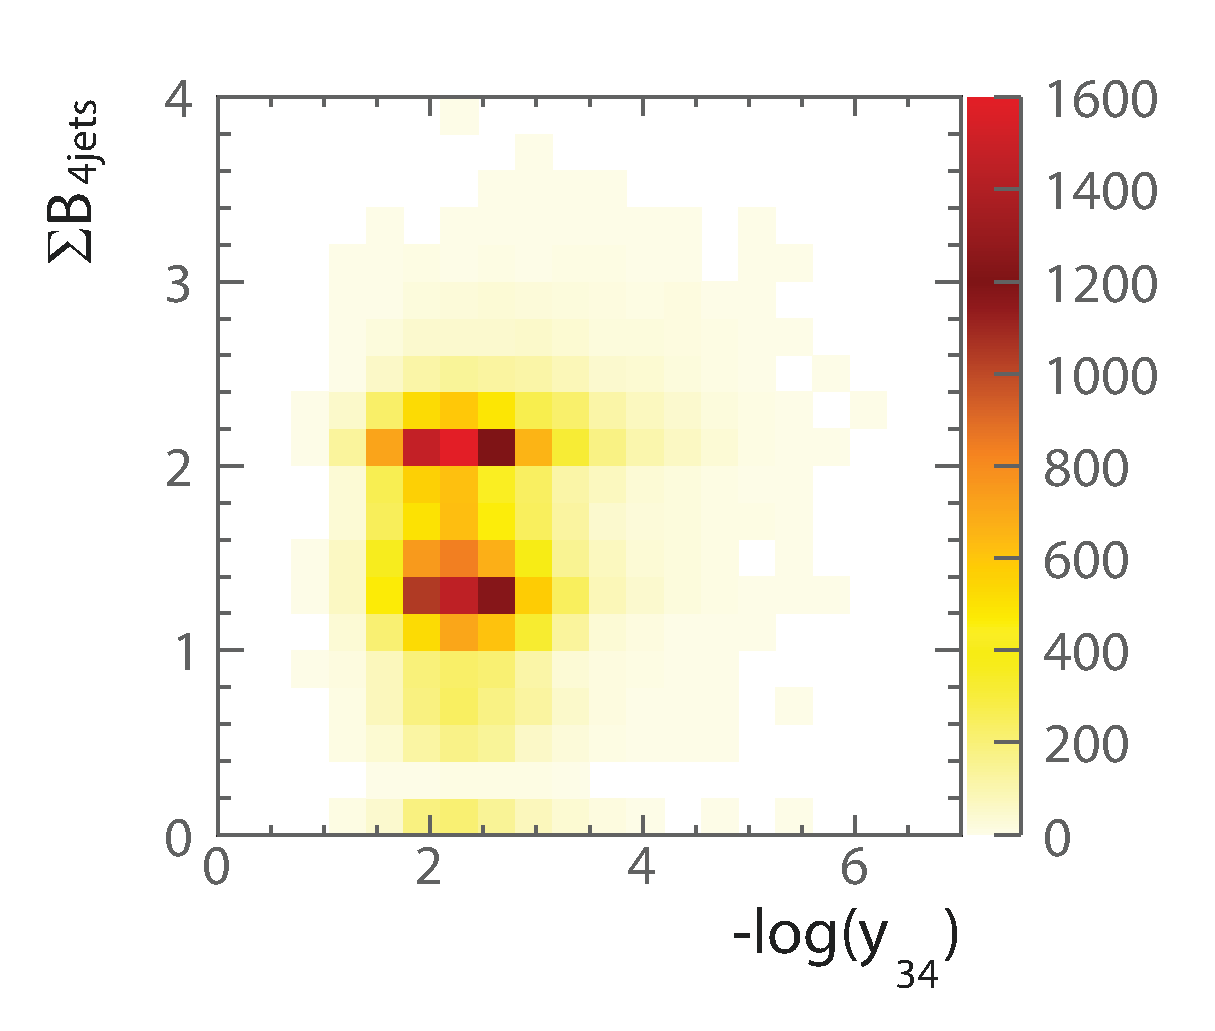
\includegraphics[width=\textwidth]{doubleHiggs/preSel/mutual6022bbWW2}
    \caption{\eeToHHbbWW, hadronic}
    \label{fig:doubleHiggs1.4MutualbbWW}
  \end{subfigure}
    \begin{subfigure}[b]{0.45\textwidth}
    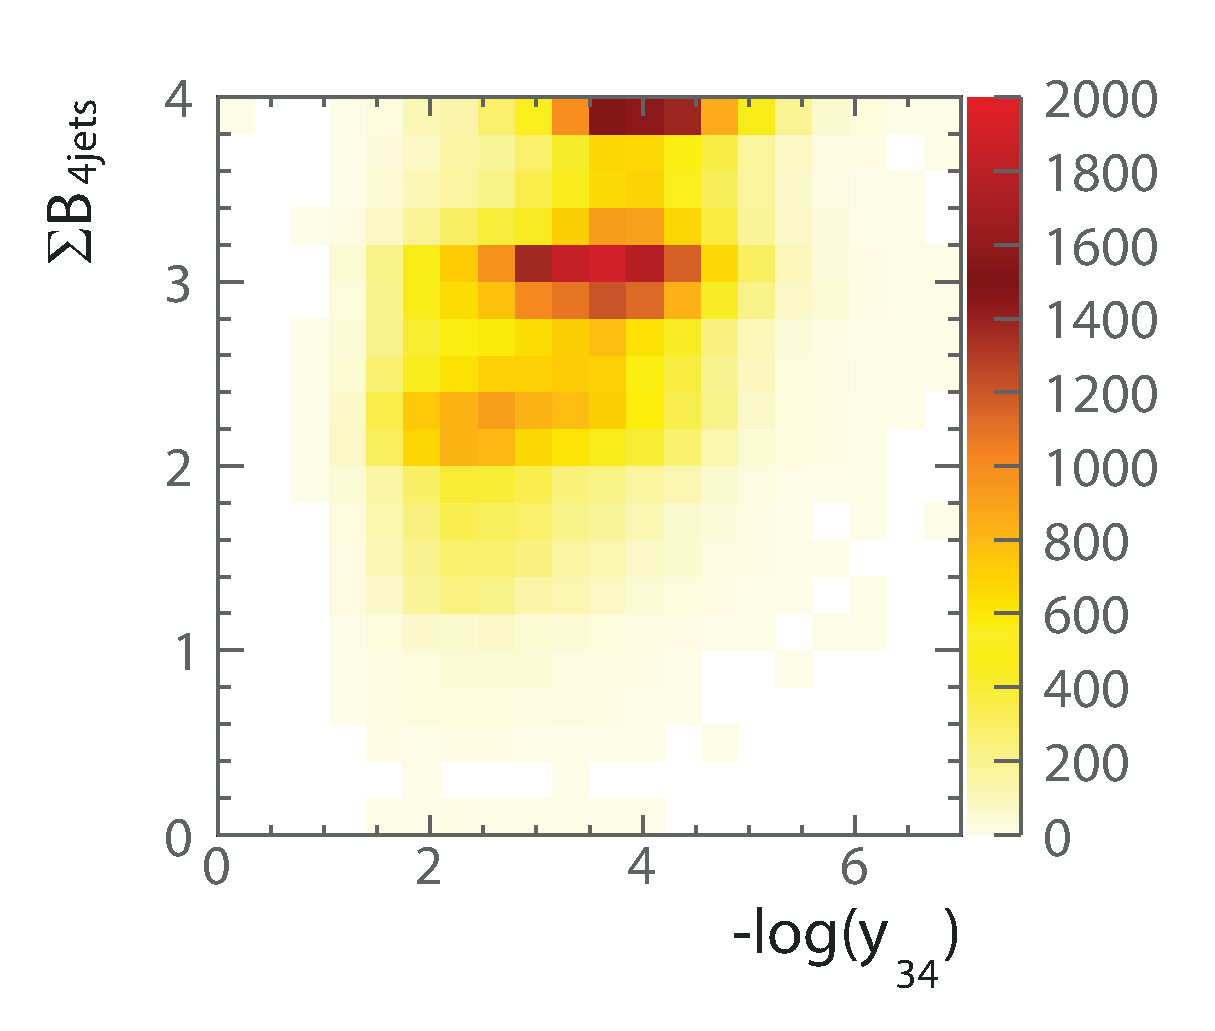
\includegraphics[width=\textwidth]{doubleHiggs/preSel/mutual6022bbbb2}
    \caption{\eeToHHbbbb}
    \label{fig:doubleHiggs1.4Mutualbbbb}
  \end{subfigure}
\caption[Sum of b-jet tag values as a function of $-\log\parenths{\y{34}}$ at \rootS{1.4}]%
   {The two-dimensional distribution of sum of b-jet tag values against $-\log\parenths{\y{34}}$ for:  a) hadronic \WW decay of \eeToHHbbWW; and b) \eeToHHbbbb events at \rootS{1.4}. The sum of b-jet tag values is calculated for the cases where events are clustered into four jets.}
   \label{fig:doubleHiggsMutualPreselection}
\end{figure}


\section{Jet pairing}

Events are reconstructed assuming the \eeToHHbbWW signal topology. The six jets are obtained from the jet re-clustering step in the \lcfiplus processor.  The next step is to group jets according to signal event topology.
Jets are paired up such that there are two jets for \HepProcess{\PHiggs \to \Pbottom \APbottom}, two jets for hadronic decay of a \PW, and two jets  for hadronic decay  of a \W*. In addition, the two $\PW$s should be from the  \PHiggs boson decay.

Six jets are associated to \Hbb, \PW and \W*. There are 90 possible permutations for associating six jets to \Hbb, \PW and \W*. The best permutation is obtained by choosing the permutation that gives the smallest $\chi^2$  quantity, representing the consistency of the hypothesis with the signal topology:
\begin{equation}
	\chi^2 = \left(\frac{m_{ij}-\mu_{\Hbb}}{\sigma_{\Hbb}^{\prime}}\right)^2 + \left(\frac{m_{klmn}-\mu_{\HWW}}{\sigma_{\HWW}^{\prime}}\right)^2  + \left(\frac{m_{kl}-\mu_{\PW}}{\sigma_{\PW}^{\prime}}\right)^2,
%\label{eqn:eq_chi2_HHWWbb}
\end{equation}
where the indices represent the six jets. The parameter $\mu$ and $\sigma^{\prime}$ are the expected peak and (asymmetric) width of the reconstructed mass distributions given in \Table{tab:doubleHiggsFitParameters}, defined as:
\begin{equation}
	\sigma_{\Hbb}^{\prime}=
    \begin{cases}
      \sigma_{L,\Hbb}, & \text{if}\ m_{ij} < \mu_{\Hbb}, \\
     \sigma_{R,\Hbb}, & \text{otherwise}, \\
   \end{cases}
   \,\text{etc.}
\end{equation}

\begin{comment}
\begin{equation}
	\sigma_{\HWW}^{\prime}=
    \begin{cases}
      \sigma_{L,\HWW}, & \text{if}\ m_{klmn} < \mu_{\HWW}\\
     \sigma_{R,\HWW}, & \text{otherwise} \\
   \end{cases}
\end{equation}


\begin{equation}
	\sigma_{\PW}^{\prime}=
    \begin{cases}
      \sigma_{L,\PW}, & \text{if}\ m_{kl} < \mu_{\PW}\\
     \sigma_{R,\PW}, & \text{otherwise} \\
   \end{cases}
\end{equation}
\end{comment}
A jet pairing is only considered when at least one of the jets associated to the \Hbb decay has a b-jet tag > 0.2. Of these combinations of jets, the jet pairing giving smallest  $\chi^2$ is selected. \FIGURE{fig:doubleHiggsJetPairing} shows the normalised distributions of $m_{\Hbb}$ after jet pairing, for the signal process, \eeToHHbbWW and the sum of all background processes. For the signal process, the distribution peaks around the expected mass of $m_{\Hbb}$. Around 1\% of signal events have no solutions for the jet pairing, i.e. no jet has a b-jet tag > 0.2. These events are no longer considered in the analysis. The full list of fraction of events surviving after this jet pairing selection are listed in \Table{tab:doubleHiggs1.4TeVPreslection} for signal \eeToHHbbWW process and all background processes.


\begin{figure}[!htbp]
 \begin{subfigure}[b]{0.45\textwidth}
    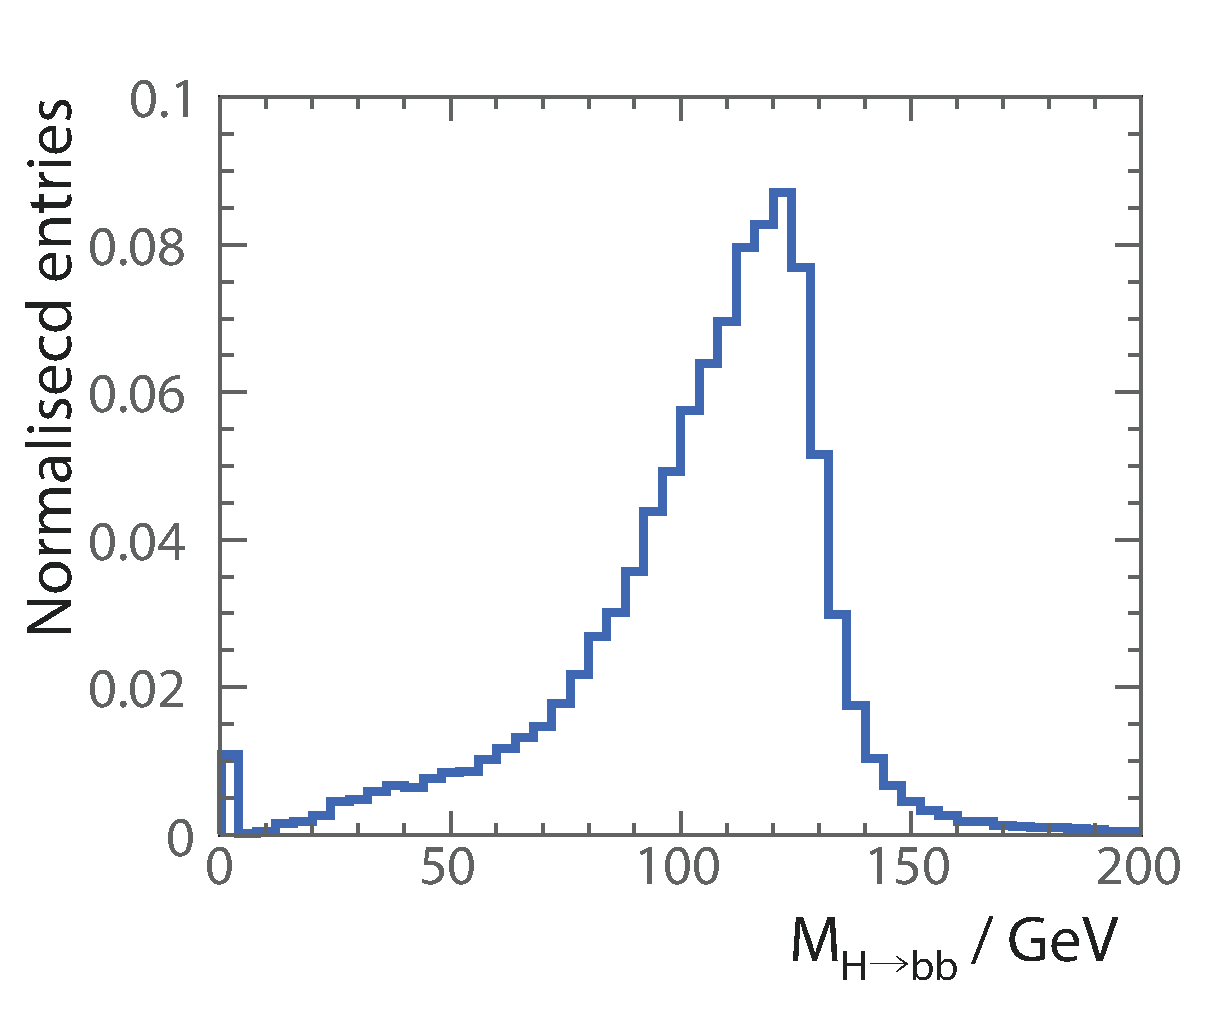
\includegraphics[width=\textwidth]{{doubleHiggs/jetPairing/nR0_7_6jet_btag2_Higgs1_M_TMVA20170223R0_7_qq_btag2_prepare2}}
    \caption{Signal}
    \label{fig:doubleHiggsJetPairingSignal}
  \end{subfigure}
 \begin{subfigure}[b]{0.45\textwidth}
    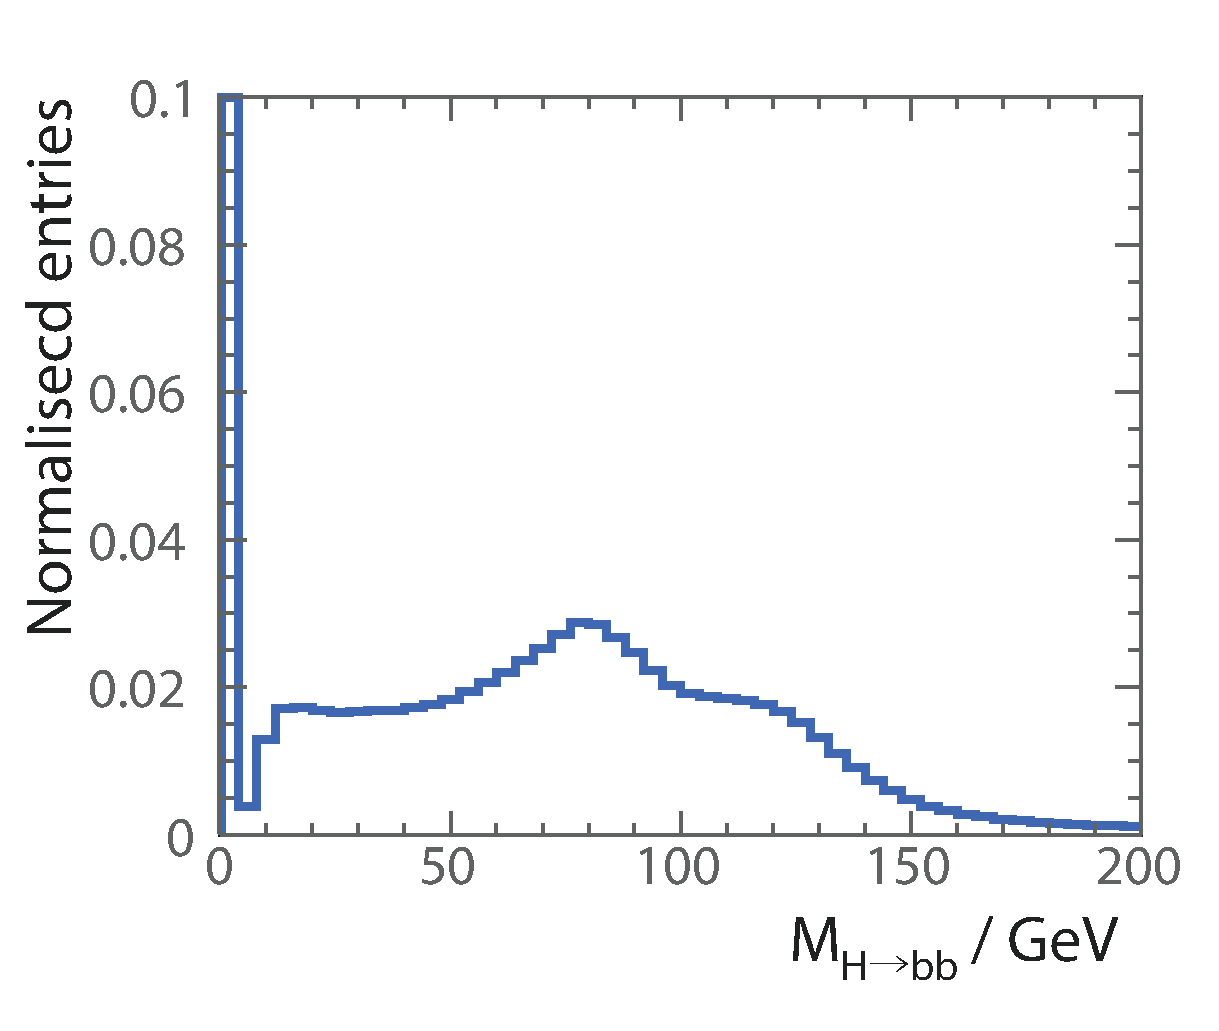
\includegraphics[width=\textwidth]{{doubleHiggs/jetPairing/nR0_7_6jet_btag2_Higgs1_M_TMVA20170223R0_7_qq_btag2_prepare_bkg2}}
    \caption{Background}
   \label{fig:doubleHiggsJetPairingBackground}
  \end{subfigure}
\caption
   {The distribution of $m_{\Hbb}$ for: a) the signal process, hadronic \WW decay of \eeToHHbbWW; and b) the sum of all background processes normalised to the respective cross sections. The area under the curve is normalised to unity. All plots are shown for \rootS{1.4}.}
   \label{fig:doubleHiggsJetPairing}
\end{figure}


\begin{table}[!htbp]\centering
% TODO fix lumi correction for e gamma, gamma e
% TODO change some of sample cross section for  electron-photon interaction with four quarks and a neutrino final state
%\small{
\small
\begin{tabular}{lrrrr}
\hline \hline
 \multicolumn{1}{L{3.5cm}}{\rootS{1.4}} &  \multicolumn{1}{R{2cm}}{N}  & \multicolumn{1}{R{2cm}}{Lepton veto} & \multicolumn{1}{R{2cm}}{\bbWW / \bbWW separation} & \multicolumn{1}{R{2cm}}{Valid jet Pairing} \\
\hline
\eeToHH $\to$ \\
\HepProcess{ \Pbottom \APbottom \PWplus \PWminus \Pnue \APnue}, hadronic             &27.9& 89.7\% & 79.1\% & 78.3\%\\
\hline
\eeToHH $\to$ \\
\HepProcess{ \Pbottom \APbottom \Pbottom \APbottom \Pnue \APnue}             &67.6& 90.8\% & 18.0\% & 18.0\% \\
\eeToHH $\to$ other & 128.0 & 40.8\% & 35.8\% & 31.2\% \\
\hline
\eeTo{\qlight \qlight \PHiggs \Pnu \APnu}  & 1290 & 72.8\% & 69.7\% & 57.7\%\\
\eeTo{\Pcharm \APcharm \PHiggs \Pnu \APnu}  & 540 & 74.7\%& 59.8\%& 52.7\%\\
\eeTo{\Pbottom \APbottom \PHiggs \Pnu \APnu}  & 465 & 74.3\%& 32.2\%& 31.8\%\\

\eeTo{ \Pquark \Pquark \Pquark \Pquark}   &   1867650& 79.9\% & 64.0\%& 38.6\%\\
\eeTo{ \Pquark \Pquark \Pquark \Pquark \Plepton \Plepton}& 93150 & 8.9\%& 8.2\%& 4.7\%\\
\eeTo{ \Pquark \Pquark \Pquark \Pquark \Plepton \Pnu}& 165600 & 16.5\%& 14.6\%& 13.3\%\\
\eeTo{ \Pquark \Pquark \Pquark \Pquark \Pnu \APnu} & 34800& 87.6\%& 82.0\%& 46.8\%\\

\eeTo{ \Pquark \Pquark} &  6014250 & 81.0\%& 57.8\%& 39.0\%\\
\eeTo{ \Pquark \Pquark \Plepton \Pnu} &  6464550 & 22.5\%& 17.0\%& 10.5\%\\
\eeTo{ \Pquark \Pquark \Pl \Pl} &  4088700 & 19.4\%& 18.6\%& 12.4\%\\
\eeTo{ \Pquark \Pquark \Pnu \Pnu} & 1181550 & 91.8\%& 74.0\%& 47.3\% \\
\hline
\egamma{\Pepm}{\Pphoton}{\BS}{\Pepm \Pquark \Pquark \Pquark \Pquark} & 2606625  & 34.2\%& 33.5\%& 22.9\%\\
%\egamma{\Pem}{\Pphoton}{BS}{\Pem \Pquark \Pquark \Pquark \Pquark} & 1305787.5  & 34.0\%& 33.3\%& 22.8\%\\
%\egamma{\Pep}{\Pphoton}{BS}{\Pep \Pquark \Pquark \Pquark \Pquark} & 1300837.5 & 34.3\%& 33.6\%& 22.9\%\\
\egamma{\Pepm}{\Pphoton}{\EPA}{\Pepm \Pquark \Pquark \Pquark \Pquark} & 861000.0 & 16.4\%& 15.8\%& 10.7\%\\
%\egamma{\Pem}{\Pphoton}{EPA}{\Pem \Pquark \Pquark \Pquark \Pquark} & 430650.0 & 16.4\%& 15.8\%& 10.7\%\\
%\egamma{\Pep}{\Pphoton}{EPA}{\Pep \Pquark \Pquark \Pquark \Pquark}  & 430350.0 & 16.3\% & 15.8\%& 10.7\%\\
\egamma{\Pepm}{\Pphoton}{\BS}{\Pnu \Pquark \Pquark \Pquark \Pquark}& 178987.5  & 85.6\%& 81.3\%& 54.4\%\\
%\egamma{\Pem}{\Pphoton}{BS}{\Pnu \Pquark \Pquark \Pquark \Pquark}& 89775.0  & 85.6\%& 81.3\%& 54.7\%\\
%\egamma{\Pep}{\Pphoton}{BS}{\APnu \Pquark \Pquark \Pquark \Pquark}& 89212.5 &.85.6\% & 81.3\%& 54.0\%\\
\egamma{\Pepm}{\Pphoton}{\EPA}{\Pnu \Pquark \Pquark \Pquark \Pquark}& 52050  & 44.5\% & 42.0\%& 27.4\%\\
%\egamma{\Pem}{\Pphoton}{EPA}{\Pnu \Pquark \Pquark \Pquark \Pquark}& 26100.0  & 44.6\% & 42.1\%& 27.6\%\\
%\egamma{\Pep}{\Pphoton}{EPA}{\APnu \Pquark \Pquark \Pquark \Pquark}& 25950.0  & 44.4\%& 41.9\%& 27.2\% \\
\egamma{\Pepm}{\Pphoton}{\BS}{\Pquark \Pquark \PHiggs \Pnu} & 35437.5  & 70.7\% & 65.0\%& 55.4\%\\
%\egamma{\Pem}{\Pphoton}{BS}{\Pquark \Pquark \PHiggs \Pnu} & 17775  & 70.6\% & 64.9\%& 55.3\%\\
%\egamma{\Pep}{\Pphoton}{BS}{\Pquark \Pquark \PHiggs \Pnu} & 17662.5  & 70.7\% & 65.0\% & 55.5\%\\
\egamma{\Pepm}{\Pphoton}{\EPA}{\Pquark \Pquark \PHiggs \Pnu} & 10170  & 37.0\% & 33.8\% & 28.8\%\\
%\egamma{\Pem}{\Pphoton}{EPA}{\Pquark \Pquark \PHiggs \Pnu} & 5085  & 36.9\% & 33.7\% & 28.7\%\\
%\egamma{\Pep}{\Pphoton}{EPA}{\Pquark \Pquark \PHiggs \Pnu} & 5085   & 37.1\% & 33.9\% & 28.9\%\\
\hline
\gammagamma{\Pphoton}{\BS}{\Pphoton}{\BS}{ \Pquark \Pquark \Pquark \Pquark}& 2054951.5  & 85.6\%& 81.3\%& 54.0\%\\
\gammagamma{\Pphoton}{\BS}{\Pphoton}{\EPA}{ \Pquark \Pquark \Pquark \Pquark}& 4521037.5  &49.6\%& 48.5\%& 32.9\%\\
\gammagamma{\Pphoton}{\EPA}{\Pphoton}{\BS}{ \Pquark \Pquark \Pquark \Pquark}& 4539150 & 49.6\%& 48.5\%& 32.9\%\\
\gammagamma{\Pphoton}{\EPA}{\Pphoton}{\EPA}{ \Pquark \Pquark \Pquark \Pquark}& 1129500 & 31.0\% & 30.1\% & 20.5\%\\
\hline \hline
\end{tabular}

\caption
{The table shows the expected number of events, before cuts and after successive cuts: the lepton veto, \eeToHHbbWW/\eeToHHbbbb separation, and valid jet pairing.  \HiggsTableLow }
\label{tab:doubleHiggs1.4TeVPreslection}
\end{table}


\section{Pre-selection}
\label{sec:doubleHiggsPreSelection}

After the association of jets to candidate bosons are made under hypothesis that an event is a signal event, kinematic and topological variables can be calculated. A set of pre-selection cuts are placed to discard the phase space dominated by background events. Cuts on \pT, b-jet tag, and invariant mass of the double Higgs system are used.

Since both Higgs bosons are on mass shell,  the invariant mass of the double Higgs system is large. Consequently, a cut on $m_{\HH} > 150$\,GeV, as shown in \FIGURE{fig:doubleHiggs1.4PreSelmHH}, removes a small amount of signal events, but discard lots of  background events, especially  \HepProcess{\Gammagamma \to \Pquark \Pquark \Pquark \Pquark} events.

\begin{figure}[!htbp]
    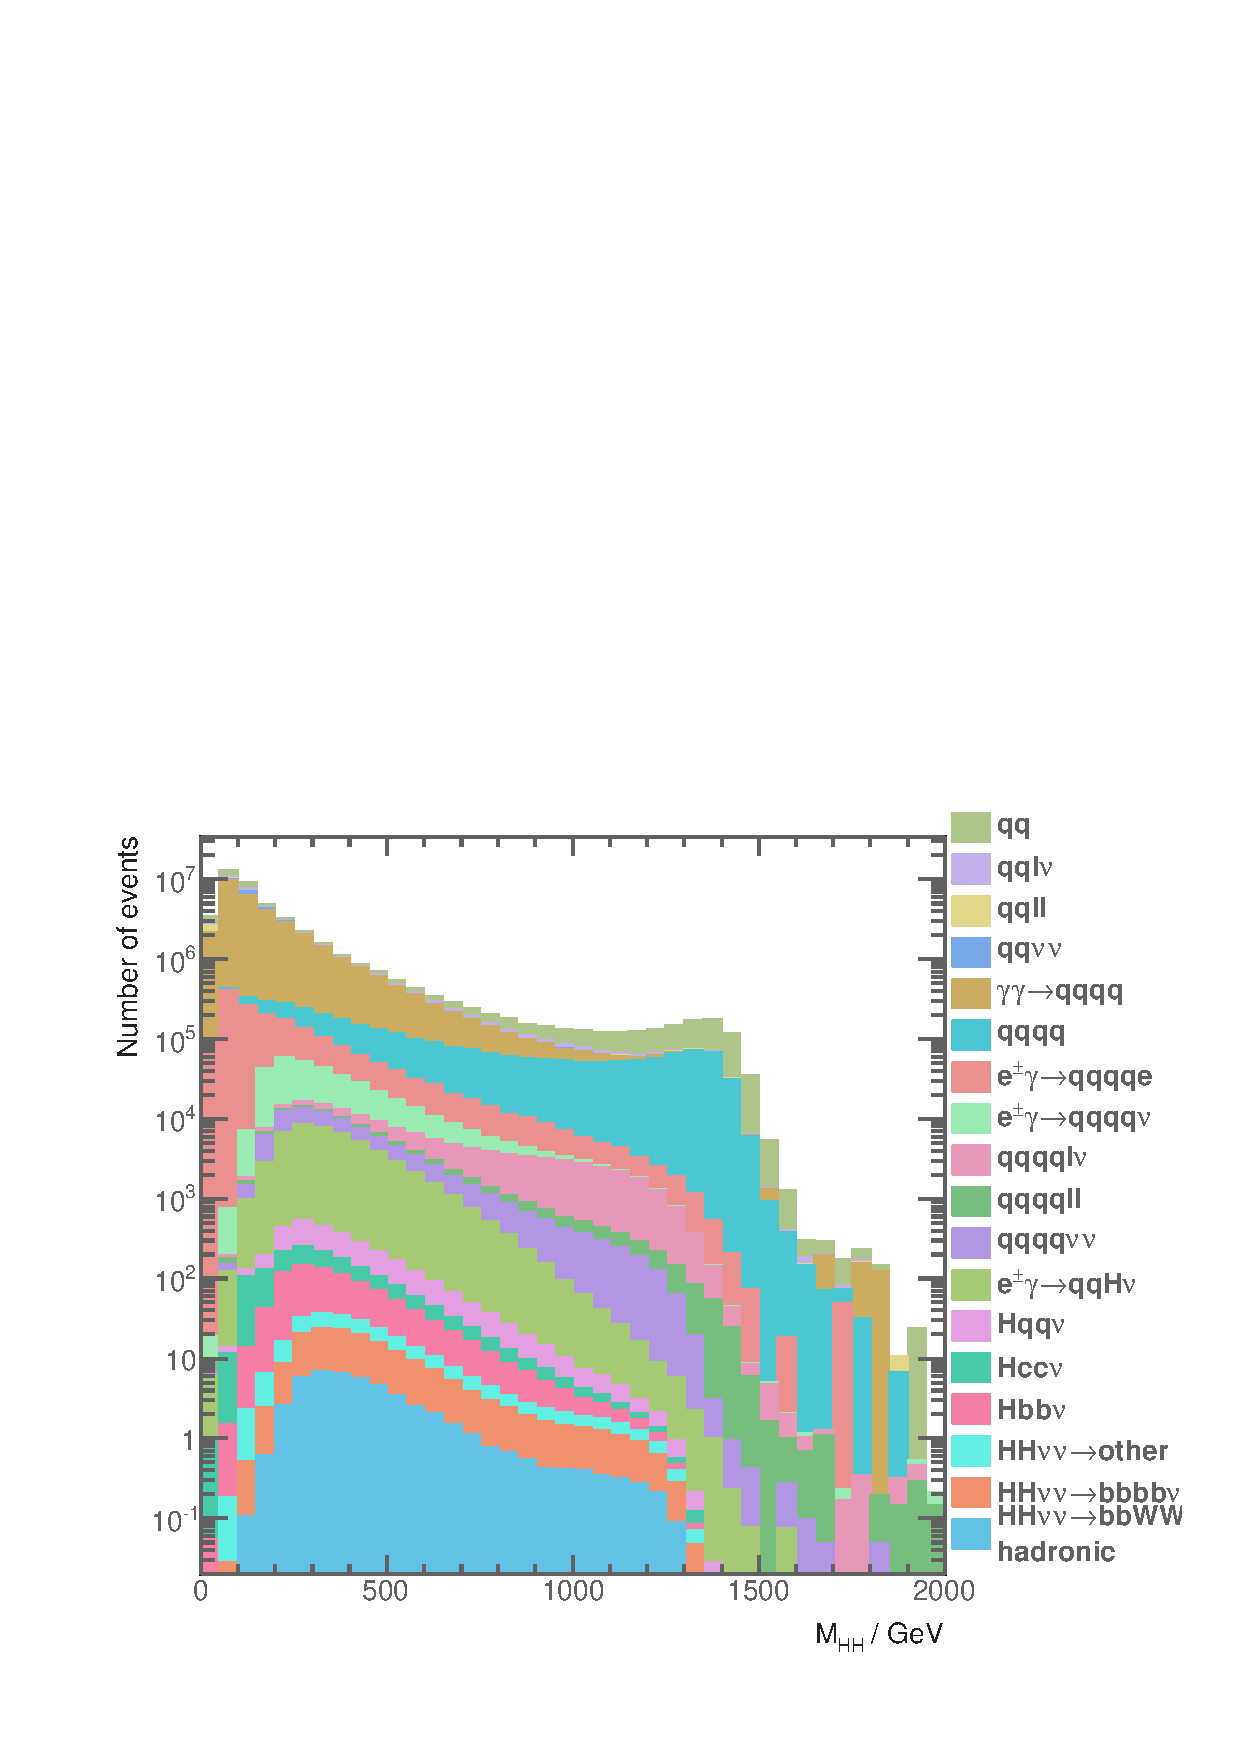
\includegraphics[width=0.95\textwidth]{{doubleHiggs/preSel2/nR0_7_6jet_btag2_Higgs_all_M_TMVA20161208R0_7_qq_btag2_prepare}.pdf}
   \caption{Distributions of the invariant mass of the two Higgs system for \rootS{1.4}, assuming an integrated luminosity of 1500\,\uprightMath{fb^{-1}}. }
    \label{fig:doubleHiggs1.4PreSelmHH}

\end{figure}


Many background events do not have \Pbottom quarks in the final state. Therefore, by requiring the second highest b-jet tag value greater than 0.2, as shown in \FIGURE{fig:doubleHiggs1.4PreSelbtag},  background events with no \Pbottom quarks in final states are removed.

\begin{figure}[!htbp]
    \includegraphics[width=0.95\textwidth]{{doubleHiggs/preSel2/nR0_7_6jet_btag2_btag2_TMVA20161208R0_7_qq_btag2_prepare}.pdf}

    \caption{Distributions of the  second highest b-jet tag value for \rootS{1.4}, assuming an integrated luminosity of 1500\,\uprightMath{fb^{-1}}. }
    \label{fig:doubleHiggs1.4PreSelbtag}
\end{figure}

The signal final states have neutrinos and hence missing momentum in the events. Therefore, the transverse  momentum  of the two Higgs system is non zero. A cut of $\pT>30$\,GeV, as shown in \Figure{fig:doubleHiggs1.4PreSelpT}, is extremely effective against background processes with no neutrinos in the final state.

\begin{figure}[!htbp]
    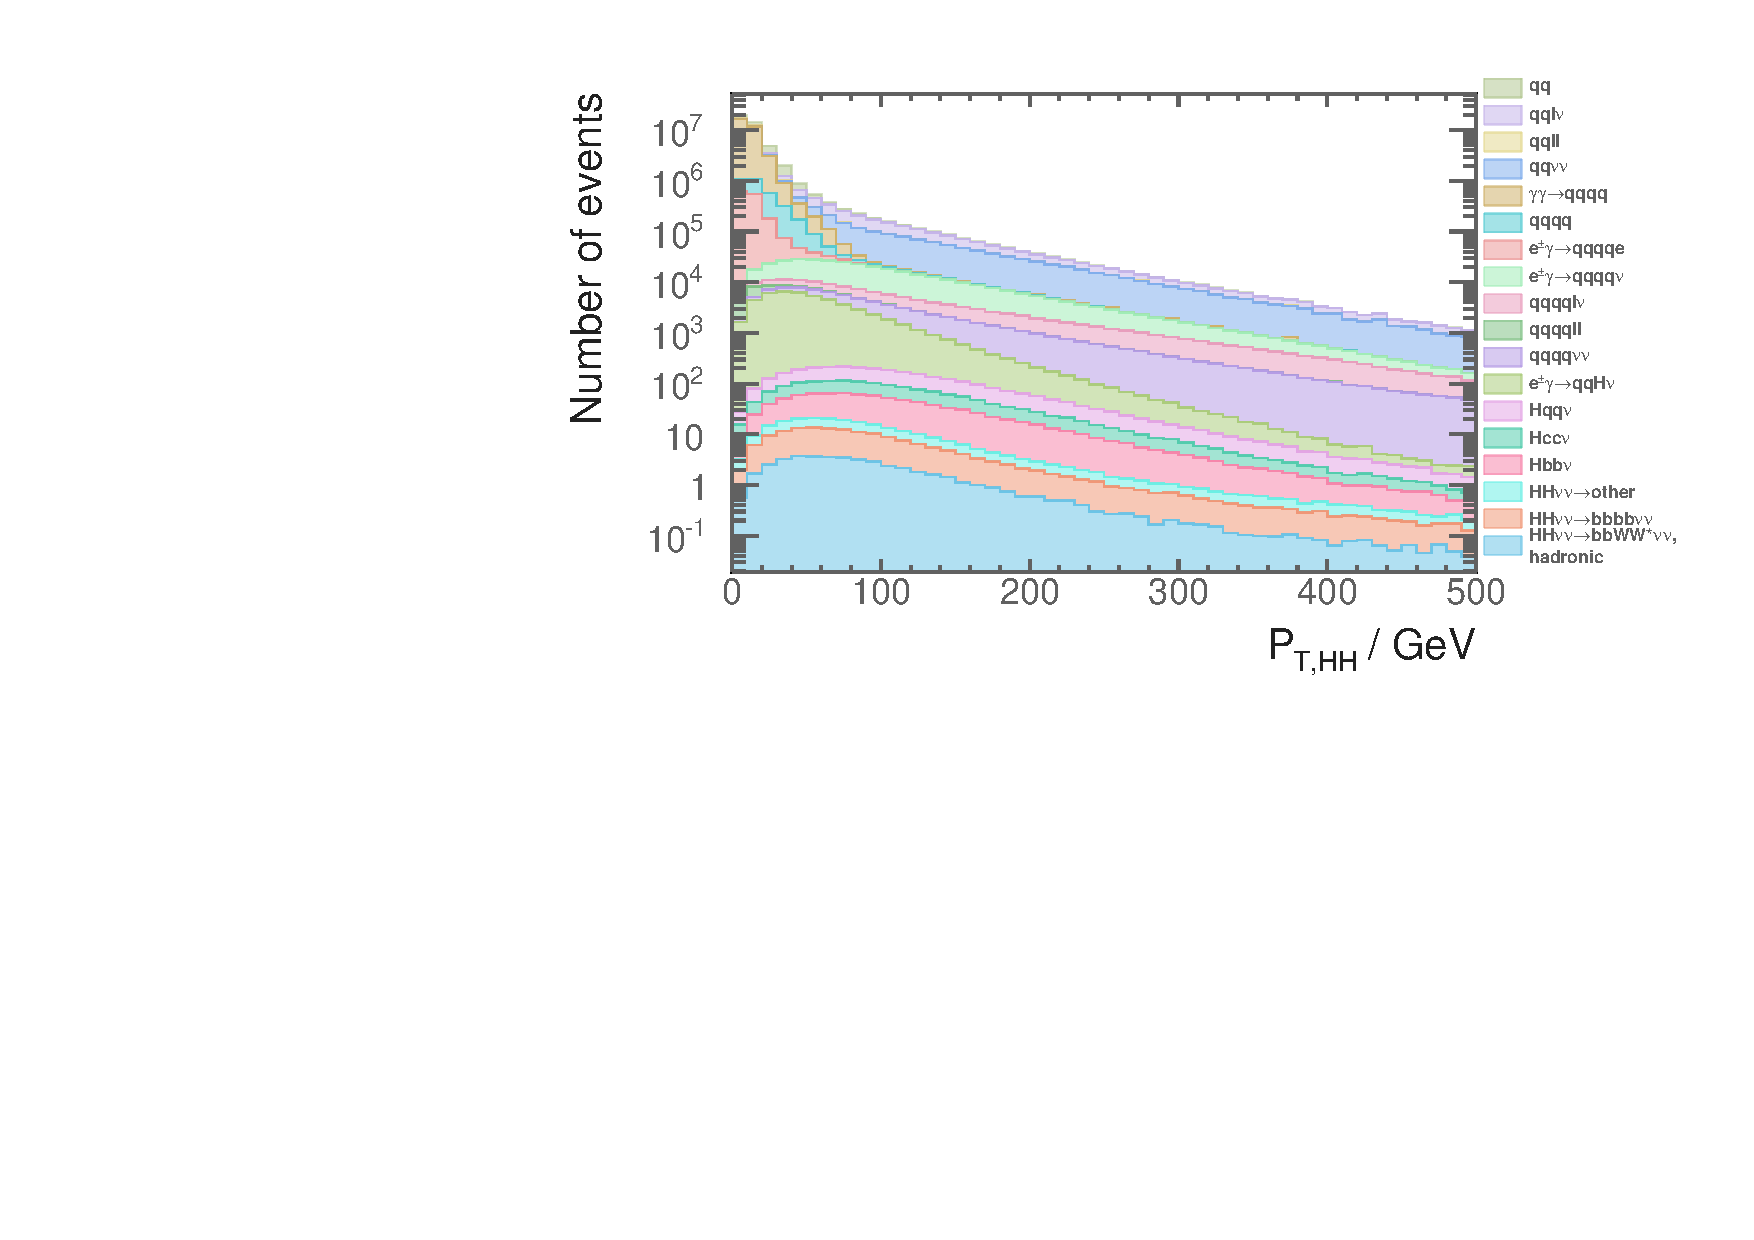
\includegraphics[width=0.95\textwidth]{{doubleHiggs/preSel2/nR0_7_6jet_btag2_Higgs_all_Pt_TMVA20161208R0_7_qq_btag2_prepare}.pdf}

    \caption{Distributions of the transverse momentum  of the two Higgs system for \rootS{1.4}, assuming an integrated luminosity of 1500\,\uprightMath{fb^{-1}}. }
    \label{fig:doubleHiggs1.4PreSelpT}
\end{figure}

The full list of fraction of events after each pre-selection cut can be found in \Table{tab:doubleHiggsPreslectionPart2}.

\begin{comment}
\begin{table}[!htbp]
\begin{tabular}{lr}
\hline
\hline
Pre-selection  &  \rootS{1.4}  \\
\hline
Discriminative pre-selection & \multicolumn{1}{R{0.5\textwidth}}{$m_{\HH} > 150\,GeV$, $B_2 > 0.2$,  $\pT_{\HH} > 30\,GeV$} \\
Loose cuts for MVA &  \multicolumn{1}{R{0.5\textwidth}}{$m_{\Hbb} < 500\,GeV$, $m_{\HWW} < 800\,GeV$, $m_{\PW} < 200\,GeV$, $m_{\HH} < 1400\,GeV$} \\
Mutually exclusive & \sumBtag{4} < 2.3, \y{34} < 3.7 \\
\hline
\hline
\end{tabular}
\caption
{Pre-selection cuts at \rootS{1.4}.}
\label{tab:doubleHiggsPreSel}
\end{table}
\end{comment}




\begin{table}[!htbp]\centering

\begin{tabular}{lrrr}
\hline \hline
 \multicolumn{1}{L{0.3\textwidth}}{Process} &  \multicolumn{1}{R{0.2\textwidth}}{$m_{HH}$>150GeV}  & \multicolumn{1}{R{0.2\textwidth}}{$B_2$>0.2} & \multicolumn{1}{R{0.2\textwidth}}{\pT>30GeV}  \\
\hline
\eeToHH $\to$ \\
\HepProcess{ \Pbottom \APbottom \PWplus \PWminus \Pnue \APnue}, hadronic             & 78.1\%& 66.3\% & 59.7\% \\
\hline
\eeToHH $\to$ \\
\HepProcess{ \Pbottom \APbottom \Pbottom \APbottom \Pnue \APnue}             &17.8\%& 17.4\% & 15.4\%  \\
\eeToHH $\to$ other & 30.5\% &23.0\% & 20.5\%  \\
\hline
\eeTo{\qlight \qlight \PHiggs \Pnu \APnu}  & 56.8\% &42.3\% & 39.5\% \\
\eeTo{\Pcharm \APcharm \PHiggs \Pnu \APnu}  & 44.8\% & 34.1\% & 31.7\%\\
\eeTo{\Pbottom \APbottom \PHiggs \Pnu \APnu}  & 30.7\% &27.0\% & 25.2\%\\

\eeTo{ \Pquark \Pquark \Pquark \Pquark}   & 36.1\%  &13.2\% & 3.4\%\\
\eeTo{ \Pquark \Pquark \Pquark \Pquark \Plepton \Plepton}& 4.7\% &1.5\% & 0.3\%\\
\eeTo{ \Pquark \Pquark \Pquark \Pquark \Plepton \Pnu}& 13.2\%. &10.7\% & 9.8\%\\
\eeTo{ \Pquark \Pquark \Pquark \Pquark \Pnu \APnu} & 46.1\% &17.7\% & 16.6\%\\

\eeTo{ \Pquark \Pquark} &  8.1\% &3.7\% & 0.8\%\\
\eeTo{ \Pquark \Pquark \Plepton \Pnu} & 3.1\% & 1.2\% & 0.9\%\\
\eeTo{ \Pquark \Pquark \Pl \Pl} &  0.7\% &0.4\% & 0.1\%\\
\eeTo{ \Pquark \Pquark \Pnu \Pnu} & 9\% & 4.3\% & 4.0\%\\
\hline
\egamma{\Pepm}{\Pphoton}{\BS}{\Pepm \Pquark \Pquark \Pquark \Pquark} & 10.1\% & 4.1\%  & 0.4\%\\
%\egamma{\Pem}{\Pphoton}{BS}{\Pem \Pquark \Pquark \Pquark \Pquark} & 10.1\%  & 4.1\% 0.3\\
%\egamma{\Pep}{\Pphoton}{BS}{\Pep \Pquark \Pquark \Pquark \Pquark} & 10.1\% & 4.1\% & 0.4\%\\
\egamma{\Pepm}{\Pphoton}{\EPA}{\Pepm \Pquark \Pquark \Pquark \Pquark} & 5.1\% & 2.0\% & 0.3\%\\
%\egamma{\Pem}{\Pphoton}{EPA}{\Pem \Pquark \Pquark \Pquark \Pquark} & 5.1\% & 2.0\% & 0.2\%\\
%\egamma{\Pep}{\Pphoton}{EPA}{\Pep \Pquark \Pquark \Pquark \Pquark}  & 5.0\% & 2.0\% & 0.3\% \\
\egamma{\Pepm}{\Pphoton}{\BS}{\Pnu \Pquark \Pquark \Pquark \Pquark}& 53.0\%  & 28.0\% & 25.1\%\\
%\egamma{\Pem}{\Pphoton}{BS}{\Pnu \Pquark \Pquark \Pquark \Pquark}& 53.3\% & 28.3\%  & 25.3\%\\
%\egamma{\Pep}{\Pphoton}{BS}{\APnu \Pquark \Pquark \Pquark \Pquark}& 52.6\% & 27.7\% & 24.9\% \\
\egamma{\Pem}{\Pphoton}{\EPA}{\Pnu \Pquark \Pquark \Pquark \Pquark}& 26.7\% & 13.8\% & 12.5\% \\
%\egamma{\Pem}{\Pphoton}{EPA}{\Pnu \Pquark \Pquark \Pquark \Pquark}&  26.9\% & 13.9\% & 12.6\% \\
%\egamma{\Pep}{\Pphoton}{EPA}{\APnu \Pquark \Pquark \Pquark \Pquark}& 26.5\% & 13.6\%  & 12.3\% \\
\egamma{\Pepm}{\Pphoton}{\BS}{\Pquark \Pquark \PHiggs \Pnu} & 54.3\% & 40.3\%  & 30.6\% \\
%\egamma{\Pem}{\Pphoton}{BS}{\Pquark \Pquark \PHiggs \Pnu} & 54.2\% & 40.2\%  & 30.6\% \\
%\egamma{\Pep}{\Pphoton}{BS}{\Pquark \Pquark \PHiggs \Pnu} & 54.4\% & 40.4\% & 30.6\%  \\
\egamma{\Pem}{\Pphoton}{\EPA}{\Pquark \Pquark \PHiggs \Pnu} & 28.2\% & 20.9\% & 16.1\%  \\
%\egamma{\Pem}{\Pphoton}{EPA}{\Pquark \Pquark \PHiggs \Pnu} & 28.1\% & 20.9\% & 16.0\%  \\
%\egamma{\Pep}{\Pphoton}{EPA}{\Pquark \Pquark \PHiggs \Pnu} & 28.3\% & 20.9\%   & 16.1\%  \\
\hline
\gammagamma{\Pphoton}{\BS}{\Pphoton}{\BS}{ \Pquark \Pquark \Pquark \Pquark}& 23.1\% & 9.2\%  & 0.3\%\\
\gammagamma{\Pphoton}{\BS}{\Pphoton}{\EPA}{ \Pquark \Pquark \Pquark \Pquark}& 13.6\% & 5.4\%  &0.4\%\\
\gammagamma{\Pphoton}{\EPA}{\Pphoton}{\BS}{ \Pquark \Pquark \Pquark \Pquark}& 13.6\% & 5.4\% & 0.3\%\\
\gammagamma{\Pphoton}{\EPA}{\Pphoton}{\EPA}{ \Pquark \Pquark \Pquark \Pquark}& 8.6\% & 3.5\% & 0.3\% \\
\hline \hline
\end{tabular}
\caption[List of signal and background samples after pre-selection cuts at \rootS{1.4}.]
{The table shows the expected number of events after successive cuts:  invariant mass of the two Higgs system > 150\,GeV,  the  second highest b-jet tag value > 0.2, and the transverse momentum  of the two Higgs system  > 30\,GeV.  All cuts include the lepton veto, \eeToHHbbWW/\eeToHHbbbb separation, and valid jet pairing. \HiggsTableLow}
\label{tab:doubleHiggsPreslectionPart2}
\end{table}


\begin{comment}
    const TCut selectionCut3000 = "tR0_7_6jet_btag2_ChiSquared<20  && TightIsoLepTauAll_nPfo < 1 && BonoForwardElectronPhotons_nPfo < 1 && \
         tR0_7_6jet_btag2_Higgs_all_M>150  && \
       tR0_7_4jet_btag2_Higgs_all_bTag < 2.3 && tR0_7_6jet_btag2_minusLogY34 < 3.7 \
       && tR0_7_6jet_btag2_bTag1 > 0.7 &&\
        tR0_7_6jet_btag2_Higgs_all_M  < 3000 &&  tR0_7_6jet_btag2_Higgs1_M < 500 &&  tR0_7_6jet_btag2_Higgs2_M < 800 &&  tR0_7_6jet_btag2_W_Onshell_M < 200";

    const TCut selectionCut1400 = "nR0_7_6jet_btag2_ChiSquared<20  && IsoLepTauAll_nPfo < 1      && BonoForwardElectronPhotons_nPfo < 1 && nR0_7_6jet_btag2_Higgs_all_M>150 && \
        nR0_7_4jet_btag2_Higgs_all_bTag < 2.3  && nR0_7_6jet_btag2_minusLogY34 < 3.6 \
        &&  nR0_7_6jet_btag2_bTag2 > 0.2 && nR0_7_6jet_btag2_Higgs_all_Pt> 30 &&\
        nR0_7_6jet_btag2_Higgs_all_M  < 1400 &&  nR0_7_6jet_btag2_Higgs1_M < 500 &&  nR0_7_6jet_btag2_Higgs2_M < 800 &&  nR0_7_6jet_btag2_W_Onshell_M < 200";
\end{comment}


\section{MVA variables}

Having extracted information about leptons, b-jets, and jet pairing, a number of variables are used to differentiate the signal to the background events. These variables are the bases of the subsequent MVA event selection, listed in \Table{tab:doubleHiggsVaraibles}. The distributions of the four most powerful discriminators are shown in \Figure{fig:doubleHiggs1.4var}.

\subsection{Invariant mass  variables}

Four invariant masses are used in the MVA event selection: the invariant mass of  \Hbb ($m_{\Hbb}$), the invariant mass of  \HWW ($m_{\HWW}$), the invariant mass of  \PW ($m_{\PW}$), and the invariant mass of the double Higgs system ($m_{\HH}$).

After the jet pairing under the hypothesis of the signal events, the distributions of the invariant mass of the physical bosons of the signal events have peaks around the expect masses, where the distributions of the  background events do not have such resonance structure. Shown in \Figure{fig:doubleHiggs1.4varMHbb}, the distributions of the invariant mass of the \Hbb is  different to the distributions of the background events. Similarly, the distributions of the invariant mass of the \HWW, shown in \Figure{fig:doubleHiggs1.4varMHWW} have a different peak position to the distributions of the background events.  The invariant mass of the double Higgs system in the signal events is large due to the presence of two on-mass-shell Higgs bosons, which is also different to the distribution of the background events

\subsection{Energy and momentum variables}

Six energy and momentum variables participate in the MVA event selection: the energy of the off-mass-shell \PW ($E_{\W*}$), the energy of the missing momenta ($E_{mis}$), the transverse momentum of \Hbb ($\pT_{\Hbb}$), the transverse momentum of \HWW ($\pT_{\HWW}$), the transverse momentum of \PW ($\pT_{\PW}$), and the transverse momentum of the double Higgs system ($\pT_{\HH}$).

For the off-mass-shell \PW, the energy  is used instead of the invariant mass, as invariant mass distribution of \W* does not have a resonance structure. The energy of the missing momenta is powerful against background events with no neutrinos in the final states. The missing momenta is calculated by assuming the collision at \sqrtS and a beam crossing angle of 20\,mrad. Other momentum variables correspond to the same physical bosons or the double Higgs system used in  the invariant mass  variables, for the same reason that the distributions of these momentum variables are different for the signal events and the background events.


\subsection{Lab-frame angle variables}

Four lab-frame angle variables are in the MVA event selection: the pseudorapidity of the missing momenta ($\eta_{mis}$), the  acollinearity of the two jets associated with \Hbb ($\acolinearity{\Hbb}$),  the  acollinearity of the two jets associated with \HWW ($\acolinearity{\HWW}$), and the  acollinearity of the two Higgs bosons ($\acolinearity{\HH}$).

The pseudorapidity   of the missing momenta is used, instead of the polar angle, because the forward polar angles are transformed to a larger range in the pseudorapidity. The pseudorapidity of the missing momenta is defined as
\begin{equation}
\eta_{mis} \equiv  - \ln \left[ \tan \left( \frac{\theta_{mis}}{2} \right) \right],
\end{equation}
where $\theta_{mis}$ is the polar angle of the missing momenta measured in a spherical polar coordinate system.

Acollinearity is a measure of the angle between the two momenta. The definition for the acollinearity for momenta $i$ and momenta $j$ is
\begin{equation}
\acolinearity{ij} = \pi - \cos^{-1}\left(\textbf{\^{p}}_i\cdot\textbf{\^{p}}_j\right),
\end{equation}
where $\textbf{\^{p}}_i$ is the unit momentum three-vector of momenta $i$. The distribution of the \acolinearity{\Hbb}, shown in \Figure{fig:doubleHiggs1.4varAcolHbb}, peaks at the value of 0 or $\pi$ for many background events, which are not the same as the signal events. For the same reason, the distributions of $\acolinearity{\HWW}$ and $\acolinearity{\HH}$ are different for the signal and the background events.

\subsection{Boosted-frame angle variables}

The MVA event selection also uses five boosted-frame angle variables: the angle between two jets associated with \Hbb in the \Hbb decay rest frame ($\cosStar{\Hbb}$), the angle between two \PW{s} associated with \HWW in the \HWW decay rest frame ($\cosStar{\HWW}$), the angle between two jets associated with \PW in the \PW decay rest frame ($\cosStar{\PW}$), the angle between two jets associated with \W* in the \W* decay rest frame ($\cosStar{\W*}$), and the angle between two Higgs bosons in two Higgs bosons decay rest frame ($\cosStar{\HH}$).

These variables are some of the most powerful variables. For example, $\cosStar{\Hbb}$ for  the signal events has a unform distribution, shown in \Figure{fig:doubleHiggs1.4varSpinHbb}, as it is equally likely for two quarks to decay in any opening angle in the \Hbb decay rest frame. For the background events, by pairing jets under the signal event hypothesis, $\cosStar{\Hbb}$ does not have a flat distribution. The  $\cosStar{\Hbb}$ distribution for the background events peaks at 1.

\subsection{Event shape variables}

Five event shapes variables are used in the MVA event selection: the absolute value of the sphericity ($\abs{\sphericity}$), the negative logarithm of \y{23} ($-\ln(\y{23})$), the negative logarithm of \y{34} ($-\ln(\y{34})$), the negative logarithm of \y{45} ($-\ln(\y{45})$), the negative logarithm of \y{56} ($-\ln(\y{56})$).

The sphericity, \sphericity, is a measure of the spherical symmetry of the event, which will be different for the signal and background events. The sphericity is  derived from the sphericity tensor \cite{PhysRevLett.35.1609}, which is  defined as
\begin{equation}
{\bm{S}^{\alpha\beta}} = \frac{\sum_{i}p^{\alpha}_{i}p^{\beta}_{i}}{\sum_{i}\absOf{\vec{p_{i}}}^2},
\end{equation}
where $\vec{p_{i}}$ is the momentum vector of the particle $i$; index $i$ is summed over all particles in the event; and $\alpha$ and $\beta$ refer to the x, y, z coordinate axes. Eigenvalues of $\bm{S}$  tensor, denoted with $\lambda_{1}$, $\lambda_{2}$, $\lambda_{3}$, can be found via diagonalisation of the matrix $\bm{S}$. The normalisation condition requires $\lambda_{1}\!\geqslant\! \lambda_{2} \! \geqslant \! \lambda_{3}$ and $ \lambda_{1} \! + \! \lambda_{2} \! + \! \lambda_{3} \! = \! 1 $. Sphericity, \sphericity, is defined in terms of $\lambda$,
\begin{equation}
\sphericity = \frac{3}{2}\parenths{\lambda_{1} \! + \! \lambda_{2}}.
\end{equation}
\sphericity, is 0 for a perfect pencil-like back-to-back two-jet event, and 1 for a perfect spherically symmetric event.

%The \y{} parameter is a measure of the number of jets in an event.  It describes the transition of  the exclusive jet algorithm going from $N$ clustered jets to $N\!+\!1$ clustered jets. For example, $\y{23}$ would be the $d_{cut}$ value for a exclusive jet algorithm, above which the jet algorithm returns 2 jets, below which the jet algorithm returns 3 jets. Numerically the \y{} parameter is often much smaller than 1. A typically way to convert the small number to a machine acceptable range is to take the negative logarithm of the number. See \Section{sec:pandoraJetAlg} for discussion on jet algorithms and $d_{cut}$.

\subsection{\Pbottom-jet and \Pcharm-jet tag  variables}

Six b-jet and c-jet tag variables are used in the MVA event selection: the highest b-jet tag value of the two jets associated with \Hbb ($\btagFull{1}{\Hbb}$), the lowest b-jet tag value of the two jets associated with \Hbb ($\btagFull{2}{\Hbb}$), the highest b-jet tag value of the two jets associated with \PW ($\btagFull{1}{\PW}$), the highest b-jet tag value of the two jets associated with \W* ($\btagFull{1}{\W*}$), the highest c-jet tag value of the two jets associated with \Hbb ($\ctagFull{1}{\Hbb}$), and the highest c-jet tag value of the two jets associated with \PW ($\ctagFull{1}{\PW}$).

As mentioned in the flavour tagging section, these b-jet and c-jet tag variables are useful to separate the signal events from the background events which do not have \Pbottom quarks in the final states.

\subsection{Particle number  variables}

The last four variables used in the MVA event selection are the particle number  variables: the number of particles associated with \Hbb (\npfo{\Hbb}), the number of particles associated with \HWW (\npfo{\HWW}), the number of particles associated with \PW (\npfo{\PW}), the number of particles associated with \W* (\npfo{\W*}). These variables are effective to differentiate the signal events from the background events with fewer than six quarks in final states.

An optimal set of 32 variables are chosen for the best MVA performance, whilst no strong ($>80\%$) pair-wise correlation exists between any two variables. %shown in \Figure{fig:doubleHiggs1.4Corr}.

 \begin{table}[!htbp]\centering
\begin{tabular}{lr}
\hline
\hline
Category &  Variable \\
\hline
Invariant mass &  \multicolumn{1}{R{0.6\textwidth}}{$m_{\Hbb}$, $m_{\HWW}$, $m_{\PW}$, $m_{\HH}$} \\
Energy and momentum & \multicolumn{1}{R{0.6\textwidth}}{$E_{\W*}$, $E_{mis}$, $\pT_{\Hbb}$, $\pT_{\HWW}$, $\pT_{\PW}$, $\pT_{\HH}$} \\
Lab-frame angles & \multicolumn{1}{R{0.6\textwidth}}{$\eta_{mis}$, $\acolinearity{\Hbb}$, $\acolinearity{\PW}$, $\acolinearity{\HH}$} \\
Boosted-frame angles & \multicolumn{1}{R{0.6\textwidth}}{$\cosStar{\Hbb}$, $\cosStar{\HWW}$, $\cosStar{\PW}$, $\cosStar{\W*}$, $\cosStar{\HH}$} \\
Event shape & \multicolumn{1}{R{0.6\textwidth}}{$\abs{\sphericity}$, $-\ln(\y{23})$, $-\ln(\y{34})$, $-\ln(\y{45})$, $-\ln(\y{56})$} \\
\Pbottom-jet and \Pcharm-jet tag & \multicolumn{1}{R{0.6\textwidth}}{$\btagFull{1}{\Hbb}$, $\btagFull{2}{\Hbb}$, $\btagFull{1}{\PW}$, $\btagFull{1}{\W*}$, $\ctagFull{1}{\Hbb}$, $\ctagFull{1}{\PW}$} \\
 Particle number &  \multicolumn{1}{R{0.6\textwidth}}{$\npfo{\Hbb}$, $\npfo{\HWW}$, $\npfo{\PW}$, $\npfo{\W*}$} \\
\hline
\hline
\end{tabular}
\caption
{Variables used in the MVA event selection for \rootS{1.4}}
\label{tab:doubleHiggsVaraibles}
\end{table}



 \begin{figure}[!htbp]
  \begin{subfigure}[b]{0.45\textwidth}
    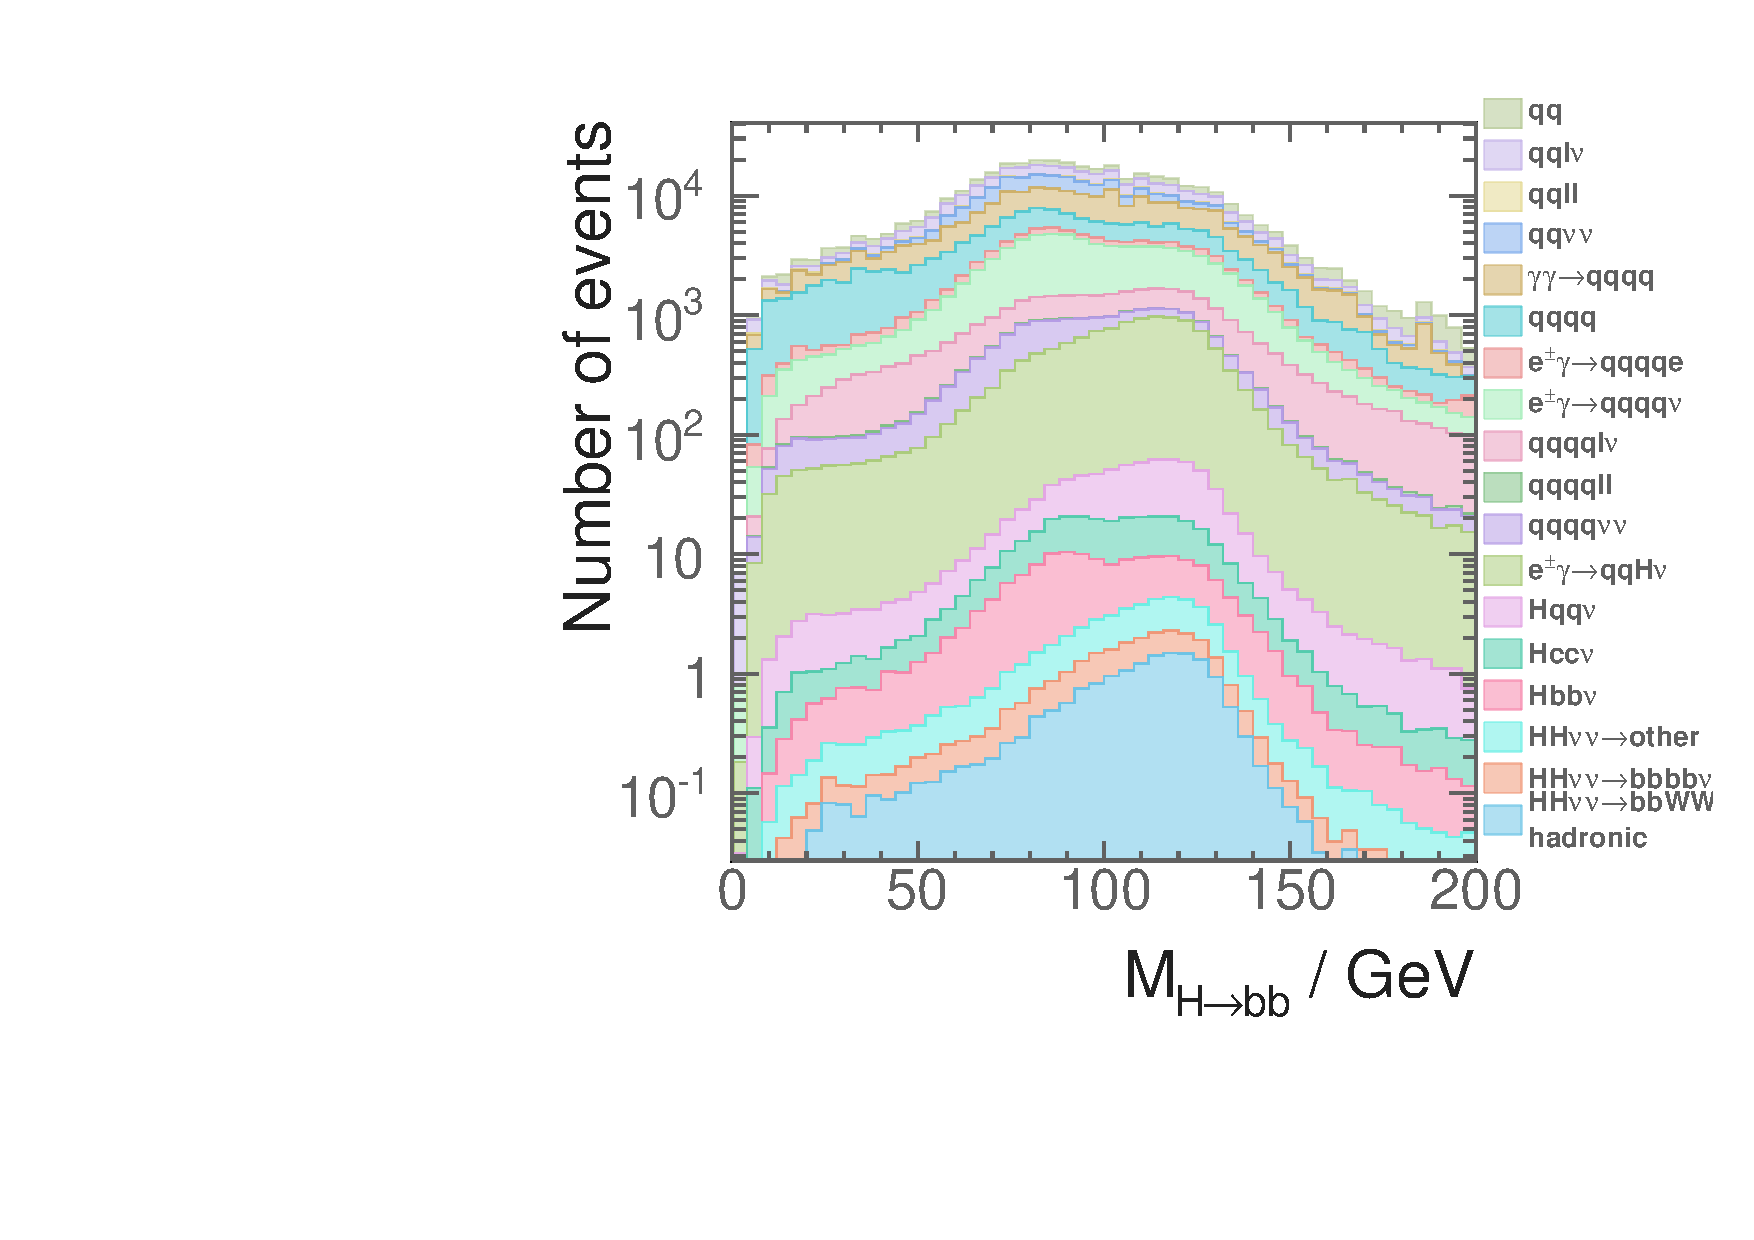
\includegraphics[width=\textwidth]{{doubleHiggs/1400var/nR0_7_6jet_btag2_Higgs1_M_TMVA20161208R0_7_qq_btag2_prepare_testNew2}.pdf}
    \caption{}
    \label{fig:doubleHiggs1.4varMHbb}
  \end{subfigure}
    \begin{subfigure}[b]{0.45\textwidth}
    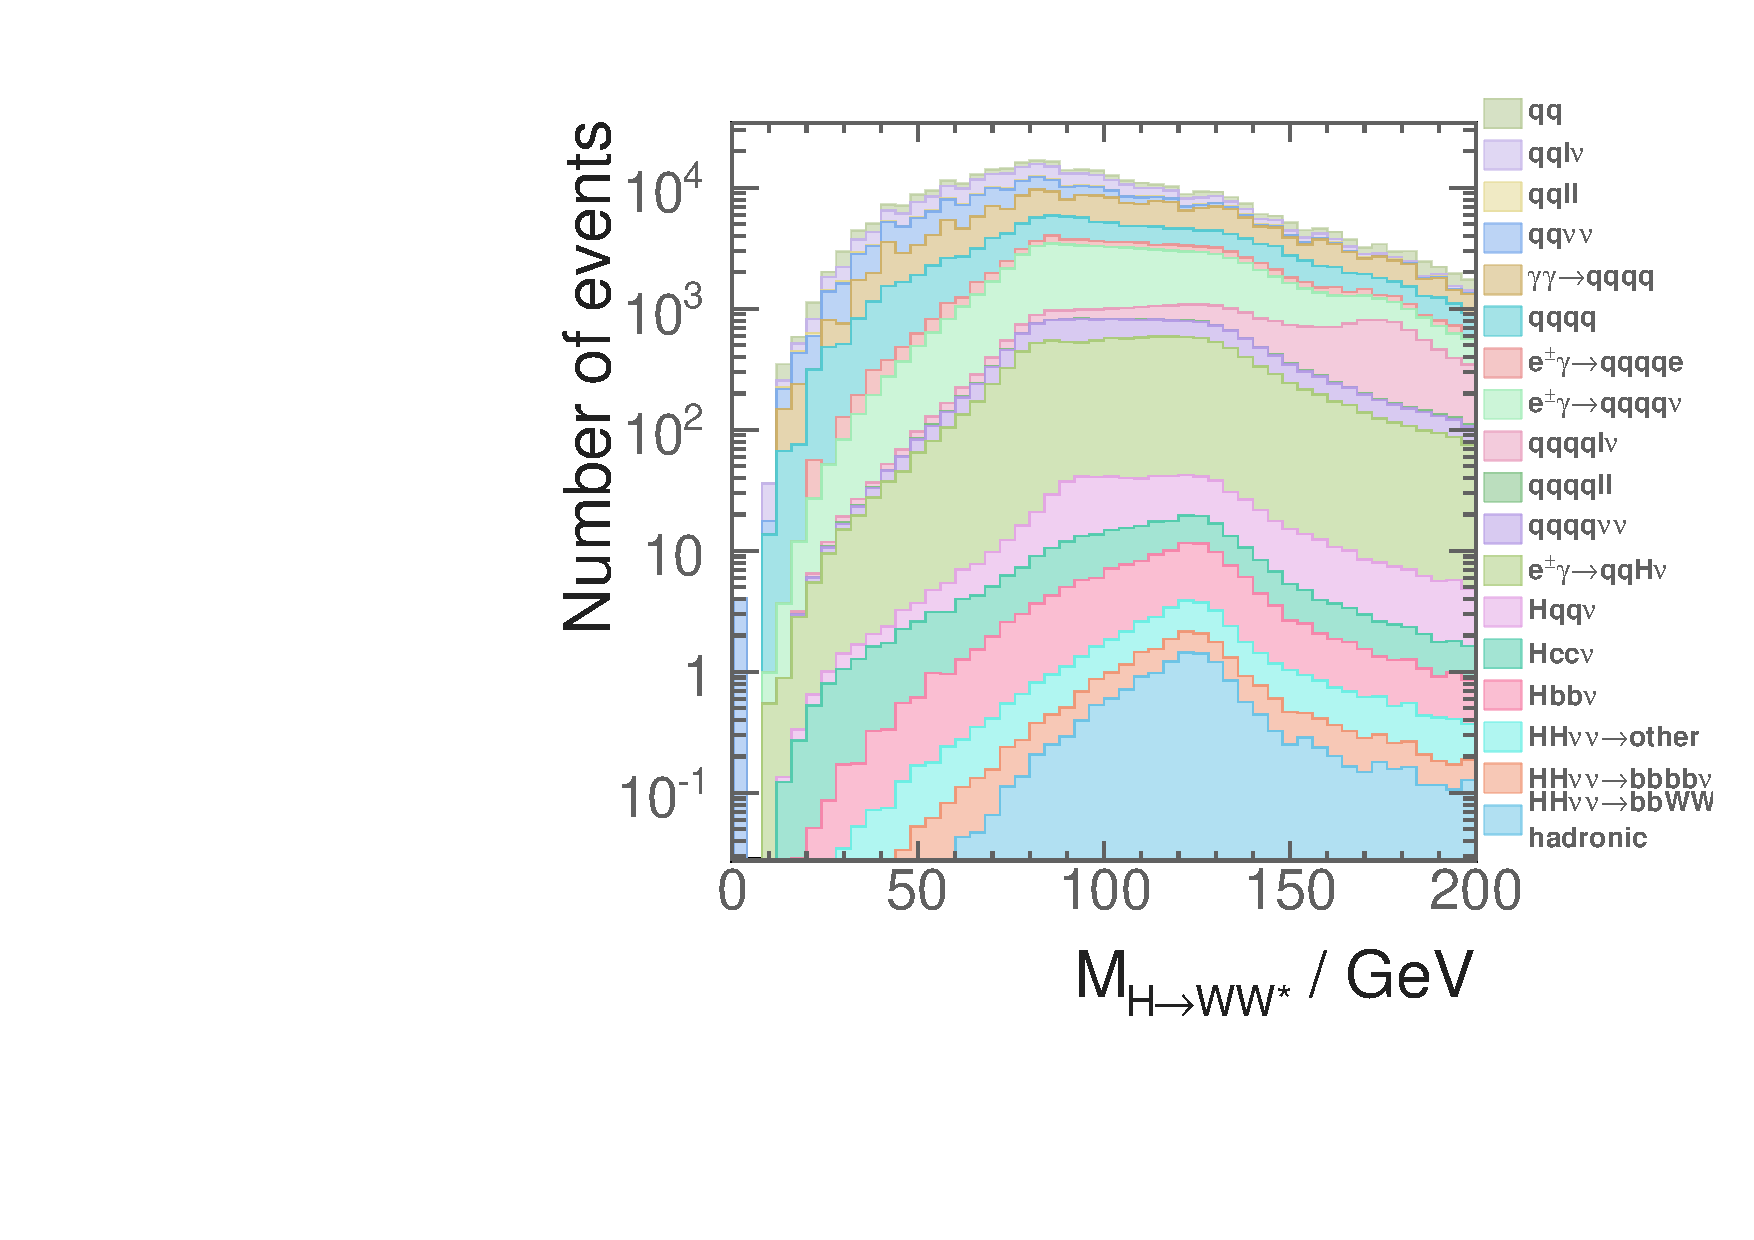
\includegraphics[width=\textwidth]{{doubleHiggs/1400var/nR0_7_6jet_btag2_Higgs2_M_TMVA20161208R0_7_qq_btag2_prepare_testNew2}.pdf}
    \caption{}
    \label{fig:doubleHiggs1.4varMHWW}
  \end{subfigure}
    \begin{subfigure}[b]{0.45\textwidth}
    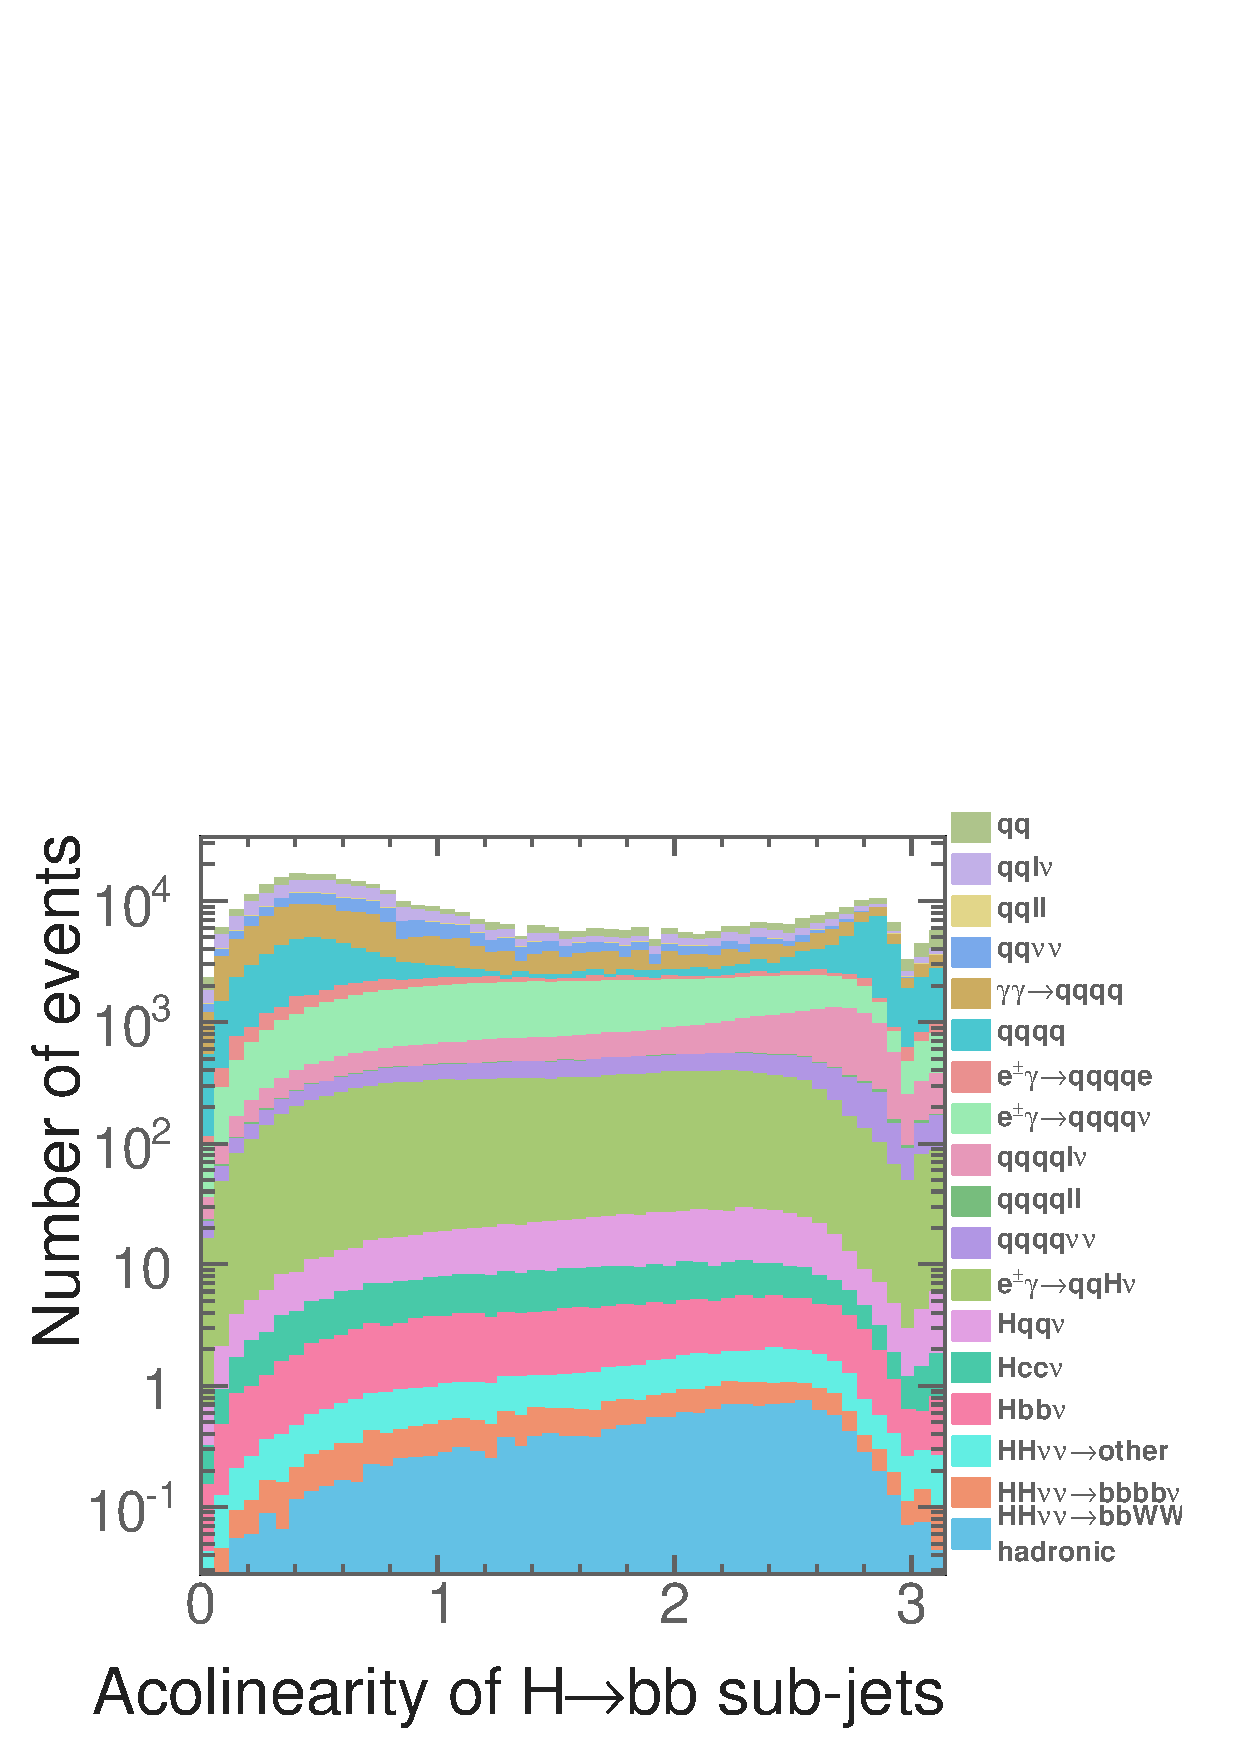
\includegraphics[width=\textwidth]{{doubleHiggs/1400var/nR0_7_6jet_btag2_Higgs1_acolinearity_TMVA20161208R0_7_qq_btag2_prepare_testNew2}.pdf}
    \caption{}
    \label{fig:doubleHiggs1.4varAcolHbb}
  \end{subfigure}
    \begin{subfigure}[b]{0.45\textwidth}
    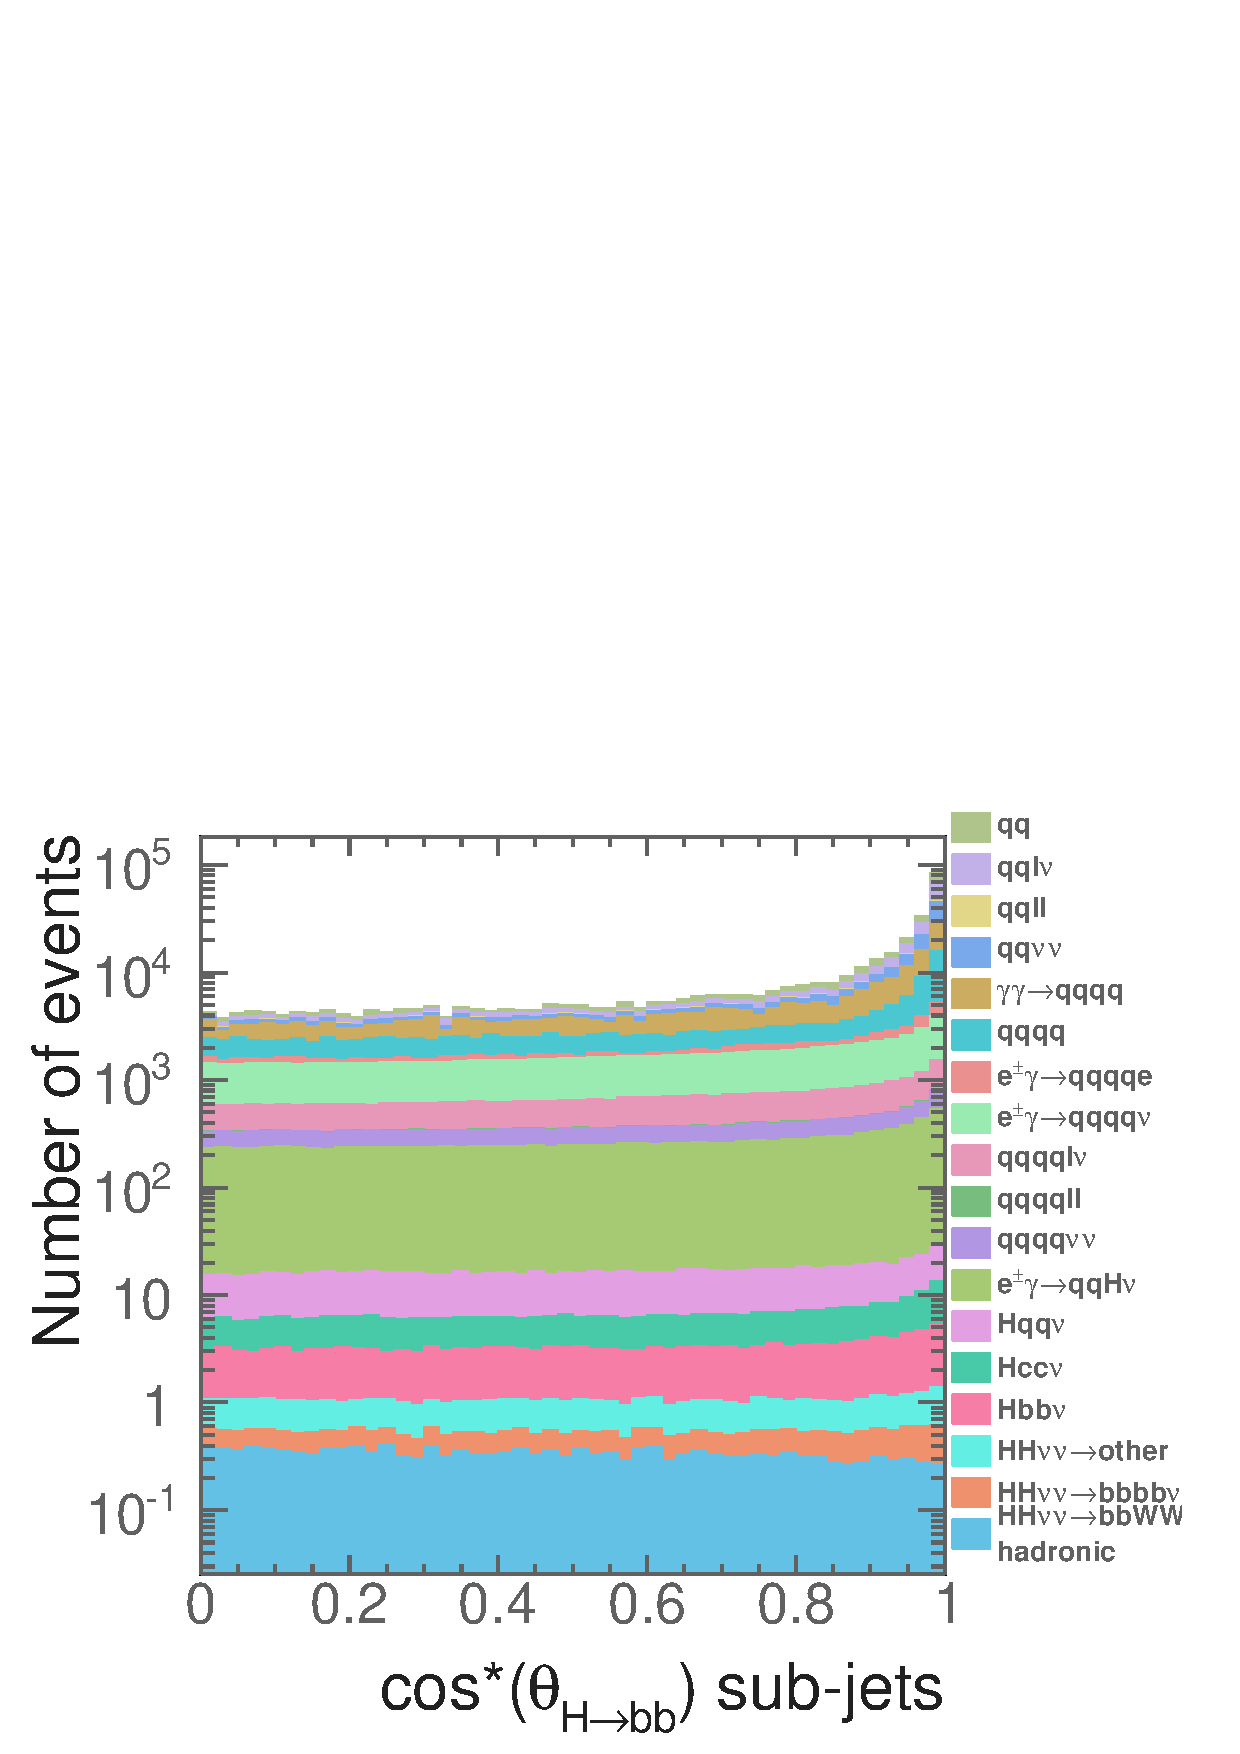
\includegraphics[width=\textwidth]{{doubleHiggs/1400var/nR0_7_6jet_btag2_Higgs1_spin_TMVA20161208R0_7_qq_btag2_prepare_testNew2}.pdf}
    \caption{}
    \label{fig:doubleHiggs1.4varSpinHbb}
  \end{subfigure}
\caption
   {Distributions of the four variables with highest discriminating power: a) the invariant mass of \Hbb; b) the invariant mas of \HWW; c) the acolinearity of the two jets associated with \Hbb; and d) the opening angle of the two jets associated with \Hbb in the decay rest frame of the \Hbb. All plots assume an integrated luminosity of  1500\,\uprightMath{fb^{-1}} at \rootS{1.4} after all pre-selection cuts applied before the MVA event selection.}
   \label{fig:doubleHiggs1.4var}
\end{figure}

\begin{comment}
 \begin{figure}[!htbp]
  \begin{subfigure}[b]{0.45\textwidth}
    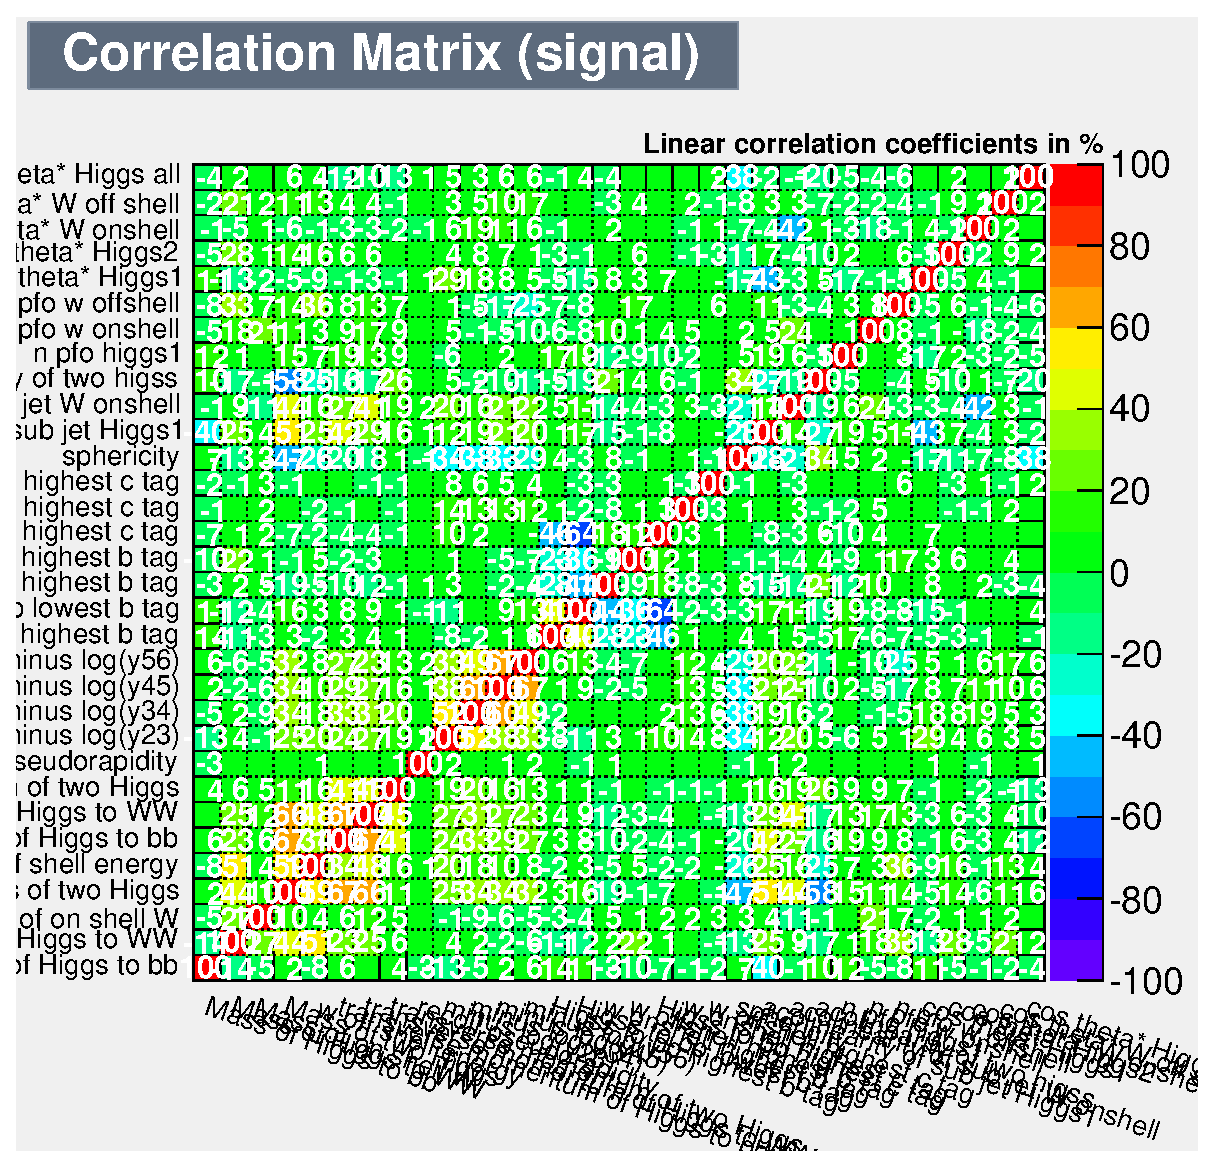
\includegraphics[width=\textwidth]{{doubleHiggs/mva/1400signalCorr}}
    \caption{}
    \label{fig:doubleHiggs1.4signalCorr}
  \end{subfigure}
    \begin{subfigure}[b]{0.45\textwidth}
    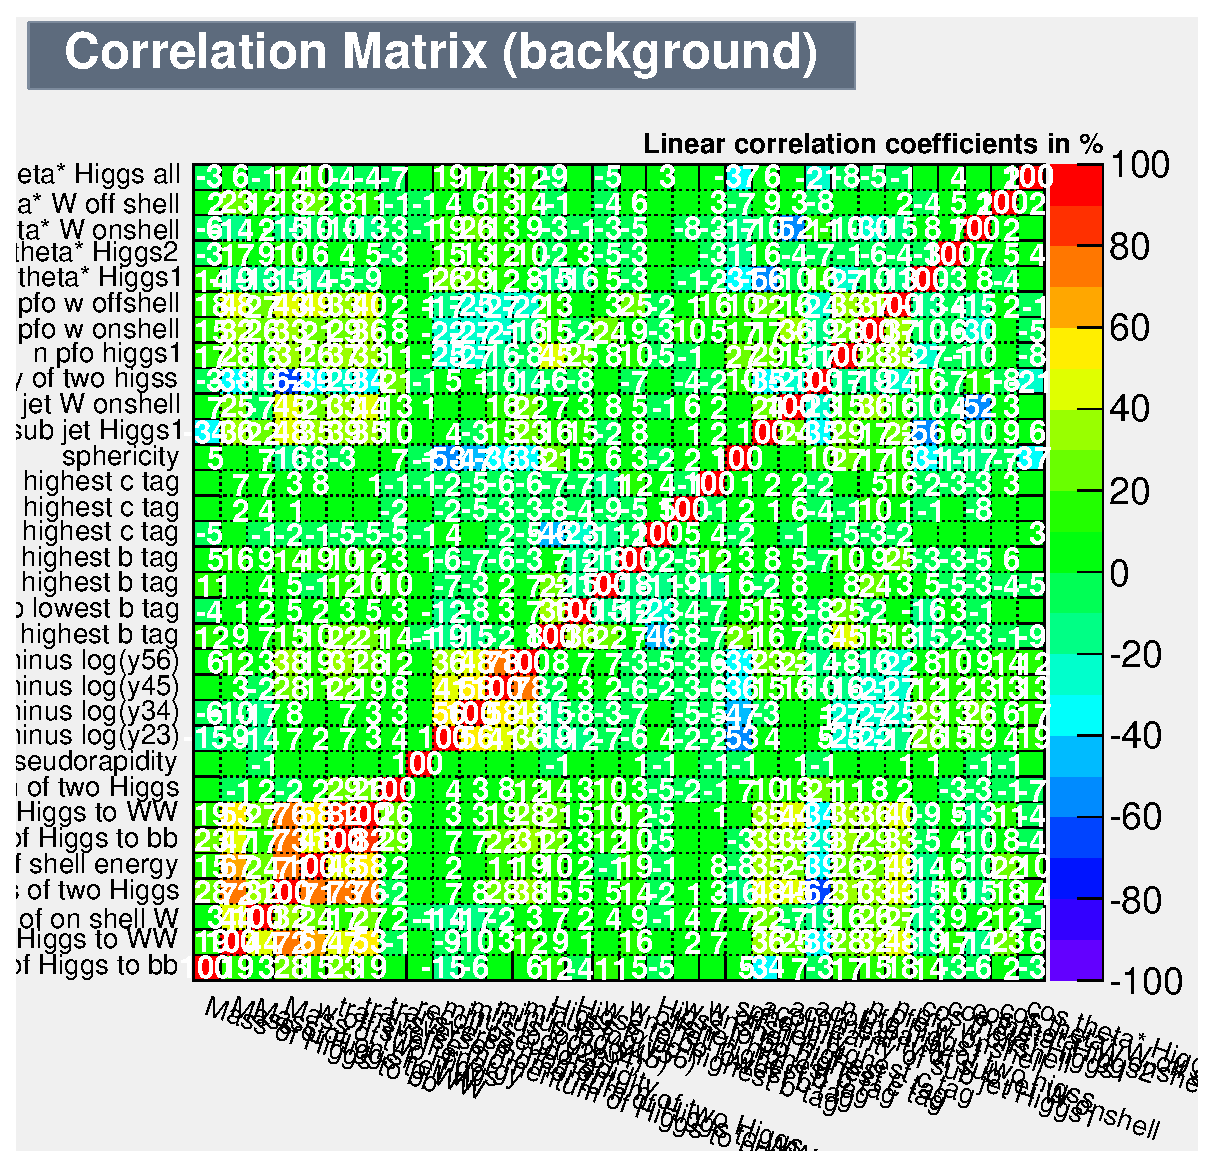
\includegraphics[width=\textwidth]{{doubleHiggs/mva/1400backgroundCorr}}
    \caption{}
    \label{fig:doubleHiggs1.4backgroundCorr}
  \end{subfigure}
\caption
   {The pair-wise correlation between discriminative variables for signal and background events at \rootS{1.4} after all pre-selection cuts.}
   \label{fig:doubleHiggs1.4Corr}
\end{figure}
\end{comment}


\subsection{Cuts to aid the MVA}

A set of cuts reduce the range of invariant masses variables in order to increase the effectiveness of the MVA event selection. Occasionally, extreme values of the invariant masses variables skew the distributions. Therefore by limiting the range of the variables, the MVA classifier could focus on the phase spaces with high event densities. The cuts require the invariant mass of the \Hbb < 500\,GeV, the invariant mass of the \HWW < 800\,GeV, the invariant mass of the \PW < 200\,GeV, and the invariant mass of the double Higgs system < 1400\,GeV.



\section{Multivariate analysis}
\label{sec:doubleHiggsMVA}
After gathering information and applying  pre-selection cuts, signal events are selected using the multivariate analysis (MVA) with Boosted Decision Tree classifier (BDT), as implemented in the \TMVA \cite{Hocker:2007ht}. The parameters of the boosted decision tree classifier were optimised and checked for overtraining, following the strategy outlined in \Section{sec:pandoraMVA}. Half of the events were used for training, and the other half used for testing and classifier optimisation. The optimised parameters are listed in \Table{tab:doubleHiggsBDTparameters}.

After dividing all events into a training set and a testing set, in the training stage of the MVA classifier, the training signal events are the  hadronic \WW decay of the \eeToHHbbWW events in the training set. The training background events are all events without double higgs production  in the training set. However, for the extraction of the \gHHH and \gWWHH,  all events with double higgs production are sensitive to the couplings Therefore, at the applying stage of the MVA classifier, all events in the testing set are used.
%, although for example, the \eeToHHbbbb final state has a different topology to the hadronic \WW decay of the \eeToHHbbWW.


%The optimisation of the BDT follows the strategy outlined in \Section{sec:pandoraMVAbdtVar}. The optimal values are obtained by choosing the best performance without overfitting.
%at \rootS{3}. The same optimised parameters are used for \rootS{1.4} analysis.

\begin{table}[!htbp]\centering
%\small{

\begin{tabular}{lr}
\hline \hline
 Parameter &  Value \\
\hline
Depth of tree & 4 \\
Number of trees & 4000 \\
The minimum number of events in a node &  0.25\% of the total events \\
Boosting & adaptive boost \\
Learning rate of the adaptive boost & 0.5 \\
Metric for the optimal cuts & Gini Index \\
Bagging fraction & 0.5 \\
Number of bins per variables & 40 \\
End node output & x $\in [0,1]$ \\
\DoPreSelection & yes \\
\hline \hline
\end{tabular}

\caption
{Optimised parameters of the boosted decision tree classifier used in the MVA event selection. See \Section{sec:pandoraMVAbdtVar} for detailed explanations of variables.}
\label{tab:doubleHiggsBDTparameters}
\end{table}

\begin{comment}
  "!H:!V:NTrees=4000:MinNodeSize=0.25%:MaxDepth=4:BoostType=RealAdaBoost:AdaBoostBeta=0.5:UseBaggedBoost:BaggedSampleFraction=0.5:SeparationType=GiniIndex:nCuts=40:DoPreselection=True" );
\end{comment}



\section{Signal selection results}
\label{sec:doubleHiggsSignalSelResult}
%first sentence doesn't make sense. Should there be an "and" in there?

Number of events passed the MVA event selection at \rootS{1.4}, assuming an integrated luminosity of 1500\,\uprightMath{fb^{-1}},  are listed in \Table{tab:doubleHiggs1.4TeVMVA} for individual processes. A few  background processes have non-zero events after the MVA event selection. \eeTo{\Pquark \APquark \PHiggs \Pnu \APnu} events are difficult to discard because its topology, one Higgs and neutrinos, is very similar to the signal event topology. Similarly, \eeTo{ \Pquark \Pquark \Pquark \Pquark \Plepton \Pnu} events can be confused with the signal events when the lepton is undetected in the forward region, or the energy of the lepton is too low for the lepton to be tagged. \eeTo{ \Pquark \Pquark \Pquark \Pquark \Pnu \APnu} events can also have a similar topology to the signal events. Other background processes that are not discarded after the MVA are the electron$-$photon and photon$-$photon interactions with the same final states as the processes above.


Before interpreting the result for analysis at \rootS{1.4}, the analyses at \rootS{3} and  the semi-leptonic channel of \eeToHH $\to$ \HepProcess{ \Pbottom \APbottom \PWplus \PWminus \Pnue \APnue} are presented.





\begin{table}[!htbp]\centering
%\small{

\begin{tabular}{lrrrr}
\hline \hline
 \multicolumn{1}{m{3.5cm}}{\rootS{1.4}} &  \multicolumn{1}{R{2cm}}{N}  & \multicolumn{1}{R{2cm}}{$\varepsilon_{presel}$} & \multicolumn{1}{R{2cm}}{$\varepsilon_{MVA}$} & \multicolumn{1}{R{2cm}}{$N_{MVA}$} \\
\hline
\eeToHH $\to$ \\
\HepProcess{ \Pbottom \APbottom \PWplus \PWminus \Pnue \APnue}, hadronic             &27.9& 59.8\% & 8.2\% & 1.29 \\
\hline
\eeToHH $\to$ \\
\HepProcess{ \Pbottom \APbottom \Pbottom \APbottom \Pnue \APnue}             &67.6& 15.4\%  & 0.5\% & 0.05\\
\eeToHH $\to$ other                             & 128.0 & 20.4\% & 1.7\% & 0.45\\
\hline
\eeTo{\qlight \qlight \PHiggs \Pnu \APnu}  & 1290 & 39.5\% & 0.05\%& 0.29\\
\eeTo{\Pcharm \APcharm \PHiggs \Pnu \APnu}  & 540 & 31.6\%& 0.1\%& 0.16\\
\eeTo{\Pbottom \APbottom \PHiggs \Pnu \APnu}  & 465 & 24.7\%& 0.3\%& 0.37\\

\eeTo{ \Pquark \Pquark \Pquark \Pquark}   &   1867650& 3.3\% & - & -\\
\eeTo{ \Pquark \Pquark \Pquark \Pquark \Plepton \Plepton}& 93150 & 0.3\%& - &  - \\
\eeTo{ \Pquark \Pquark \Pquark \Pquark \Plepton \Pnu}& 165600 & 9.8\%& 0.01\%& 2.06\\
\eeTo{ \Pquark \Pquark \Pquark \Pquark \Pnu \APnu} & 34800& 16.5\%& 0.002\% & 0.10\\

\eeTo{ \Pquark \Pquark} &  6014250 & 0.8\%& - & - \\
\eeTo{ \Pquark \Pquark \Plepton \Pnu} &  6464550 & 0.9\%&  - & - \\
\eeTo{ \Pquark \Pquark \Pl \Pl} &  4088700 & 0.08\%& - & - \\
\eeTo{ \Pquark \Pquark \Pnu \Pnu} & 1181550 & 4.0\%& - & - \\
\hline
\egamma{\Pepm}{\Pphoton}{BS}{\Pepm \Pquark \Pquark \Pquark \Pquark} & 2606625 & 0.3\%& - & -\\
%\egamma{\Pem}{\Pphoton}{BS}{\Pem \Pquark \Pquark \Pquark \Pquark} & 1305787.5  & 0.3\%& - & -\\
%\egamma{\Pep}{\Pphoton}{BS}{\Pep \Pquark \Pquark \Pquark \Pquark} & 1300837.5 & 0.4\%& -& -\\
\egamma{\Pepm}{\Pphoton}{EPA}{\Pepm \Pquark \Pquark \Pquark \Pquark} & 861000 & 0.3\%&  - &  - \\
%\egamma{\Pem}{\Pphoton}{EPA}{\Pem \Pquark \Pquark \Pquark \Pquark} & 430650.0 & 0.3\%&  - &  - \\
%\egamma{\Pep}{\Pphoton}{EPA}{\Pep \Pquark \Pquark \Pquark \Pquark}  & 430350.0 & 0.3\% & - & -\\
\egamma{\Pepm}{\Pphoton}{BS}{\Pnu \Pquark \Pquark \Pquark \Pquark}& 178987.5  & 25.7\%& 0.005\%& 2.05\\
%\egamma{\Pem}{\Pphoton}{BS}{\Pnu \Pquark \Pquark \Pquark \Pquark}& 89775.0  & 25.4\%& 0.005\%& 1.09\\
%\egamma{\Pep}{\Pphoton}{BS}{\APnu \Pquark \Pquark \Pquark \Pquark}& 89212.5 & 24.9\% & 0.004\%& 0.96\\
\egamma{\Pepm}{\Pphoton}{EPA}{\Pnu \Pquark \Pquark \Pquark \Pquark}& 52050  & 12.5\% & 0.004\% & 0.27 \\
%\egamma{\Pem}{\Pphoton}{EPA}{\Pnu \Pquark \Pquark \Pquark \Pquark}& 26100.0  & 12.6\% & - &  - \\
%\egamma{\Pep}{\Pphoton}{EPA}{\APnu \Pquark \Pquark \Pquark \Pquark}& 25950.0  & 12.4\%& 0.008\% & 0.27\\
\egamma{\Pepm}{\Pphoton}{BS}{\Pquark \Pquark \PHiggs \Pnu} & 35437.5   & 30.7\% & 0.02\% & 2.16 \\
%\egamma{\Pem}{\Pphoton}{BS}{\Pquark \Pquark \PHiggs \Pnu} & 17775   & 30.8\% & 0.02\% & 1.00 \\
%\egamma{\Pep}{\Pphoton}{BS}{\Pquark \Pquark \PHiggs \Pnu} & 17662.5  & 30.6\% & 0.02\% & 1.16 \\
\egamma{\Pepm}{\Pphoton}{EPA}{\Pquark \Pquark \PHiggs \Pnu} & 10170.0  & 16.1\% & 0.06\% & 0.95 \\
%\egamma{\Pem}{\Pphoton}{EPA}{\Pquark \Pquark \PHiggs \Pnu} & 5085  & 16.0\% & 0.04\% & 0.33 \\
%\egamma{\Pep}{\Pphoton}{EPA}{\Pquark \Pquark \PHiggs \Pnu} & 5085   & 16.2\% & 0.08\% & 0.62 \\
\hline
\gammagamma{\Pphoton}{BS}{\Pphoton}{BS}{ \Pquark \Pquark \Pquark \Pquark}& 2054951.5  & 0.2\%&  - & -\\
\gammagamma{\Pphoton}{BS}{\Pphoton}{EPA}{ \Pquark \Pquark \Pquark \Pquark}& 4521037.5  & 0.4\%& - & - \\
\gammagamma{\Pphoton}{EPA}{\Pphoton}{BS}{ \Pquark \Pquark \Pquark \Pquark}& 4539150.0 & 0.3\%&  - & - \\
\gammagamma{\Pphoton}{EPA}{\Pphoton}{EPA}{ \Pquark \Pquark \Pquark \Pquark}& 1129500.0 & 0.3\% & - & -\\
\hline \hline
\end{tabular}

\caption[Selection efficiency and number of events for signal and background at \rootS{1.4}.]%
{List of signal and background events with selection efficiency and number of events at \rootS{1.4}, assuming  an integrated luminosity  of 1500\,\uprightMath{fb^{-1}}. The number of events ($N$), the selection efficiencies of pre-selection cuts ($\varepsilon_{presel}$), the selection efficiencies of the MVA event selection after pre-selection cuts ($\varepsilon_{MVA}$), and the number of events after the MVA event selection ($N_{MVA}$) are shown. The entries marked with ``-'' represent  numbers less than 0.01. \Pquark can be \Pup, \Pdown, \Pstrange, \Pbottom or \Ptop.}
\label{tab:doubleHiggs1.4TeVMVA}
\end{table}



\section{\rootS{3} analysis}

The hadronic \WW decay of the \eeToHH $\to$ \HepProcess{ \Pbottom \APbottom \PWplus \PWminus \Pnu \APnu} at \rootS{3} analysis follows the same strategy as the analysis at \rootS{1.4}. Lepton finding, jet pairing and flavouring tagging have been discussed in previous sections. The differences, which have not been mentioned, will be highlighted in this section.

Cross sections of used samples are listed in \Table{tab:doubleHiggs3crossSection}. The mutually exclusive cuts to separate events into two independent sets are almost identical to the cuts used in the \rootS{1.4} analysis. \FIGURE{fig:doubleHiggs3TeVMutualPreselection} shows the sum of b-jet tag values, when the event is clustered into four jets, as a function of $-\log\parenths{\y{34}}$ for the hadronic \WW decay in \eeToHHbbWW and \eeToHHbbbb sub-channels. The optimised cuts are  $\sumBtag{4} < 2.3, \, -\log\parenths{\y{34}} < 3.6$. The selection efficiencies of evens after lepton veto, the  mutually exclusive cuts,  and the valid jet pairing for individual processes are shown in \Table{tab:doubleHiggs3TeVPreslection}.

\begin{table}[!htbp]\centering
% TODO fix lumi correction for e gamma, gamma e
% TODO change some of sample cross section for  electron-photon interaction with four quarks and a neutrino final state

%{

\begin{tabular}{lrr}
\hline \hline
Process  &  $\sigma(\rootS{3})$ / fb   \\
\hline
\eeToHH &0.588 \\
\hline
\eeToHHbbWWFull,hadronic &0.07 \\
\eeToHHbbbbFull  &0.19 \\
\eeToHHotherFull &0.34 \\
\hline
\eeTo{\qlight \qlight \PHiggs \Pnu \APnu} & 3.06 \\
\eeTo{\Pcharm \APcharm \PHiggs \Pnu \APnu} & 1.15\\
\eeTo{\Pbottom \APbottom \PHiggs \Pnu \APnu}  & 1.78\\

\eeTo{ \Pquark \Pquark \Pquark \Pquark} & 546.5*\\
\eeTo{ \Pquark \Pquark \Pquark \Pquark \Plepton \Plepton}&169.3*\\
\eeTo{ \Pquark \Pquark \Pquark \Pquark \Plepton \Pnu} &106.6*\\
\eeTo{ \Pquark \Pquark \Pquark \Pquark \Pnu \APnu}&71.5*\\

\eeTo{ \Pquark \Pquark} &2948.9\\
\eeTo{ \Pquark \Pquark \Plepton \Pnu} &5561.1\\
\eeTo{ \Pquark \Pquark \Pl \Pl}&3319.6\\
\eeTo{ \Pquark \Pquark \Pnu \Pnu} &1317.5 \\
\hline
\egamma{\Pepm}{\Pphoton}{\BS}{\Pepm \Pquark \Pquark \Pquark \Pquark} & 2536.3*\\
%\egamma{\Pem}{\Pphoton}{BS}{\Pem \Pquark \Pquark \Pquark \Pquark} & 1268.7*\\
%\egamma{\Pep}{\Pphoton}{BS}{\Pep \Pquark \Pquark \Pquark \Pquark}  & 1267.6*\\
\egamma{\Pepm}{\Pphoton}{\EPA}{\Pepm \Pquark \Pquark \Pquark \Pquark}  & 575.7*\\
%\egamma{\Pem}{\Pphoton}{EPA}{\Pem \Pquark \Pquark \Pquark \Pquark}  & 287.9*\\
%\egamma{\Pep}{\Pphoton}{EPA}{\Pep \Pquark \Pquark \Pquark \Pquark}   & 287.8*\\
\egamma{\Pepm}{\Pphoton}{\BS}{\Pnu \Pquark \Pquark \Pquark \Pquark}  & 524.8*\\
%\egamma{\Pem}{\Pphoton}{BS}{\Pnu \Pquark \Pquark \Pquark \Pquark}  & 262.5*\\
%\egamma{\Pep}{\Pphoton}{BS}{\APnu \Pquark \Pquark \Pquark \Pquark} & 262.3*\\
\egamma{\Pepm}{\Pphoton}{\EPA}{\Pnu \Pquark \Pquark \Pquark \Pquark}  & 108.4*\\
%\egamma{\Pem}{\Pphoton}{EPA}{\Pnu \Pquark \Pquark \Pquark \Pquark}  & 54.2*\\
%\egamma{\Pep}{\Pphoton}{EPA}{\APnu \Pquark \Pquark \Pquark \Pquark}& 54.2*\\
\egamma{\Pepm}{\Pphoton}{\BS}{\Pquark \Pquark \PHiggs \Pnu}   & 117.1* \\
%\egamma{\Pem}{\Pphoton}{BS}{\Pquark \Pquark \PHiggs \Pnu}   & 58.6* \\
%\egamma{\Pep}{\Pphoton}{BS}{\Pquark \Pquark \PHiggs \Pnu}  & 58.5* \\
\egamma{\Pepm}{\Pphoton}{\EPA}{\Pquark \Pquark \PHiggs \Pnu} & 22.4* \\
%\egamma{\Pem}{\Pphoton}{EPA}{\Pquark \Pquark \PHiggs \Pnu} & 11.7* \\
%\egamma{\Pep}{\Pphoton}{EPA}{\Pquark \Pquark \PHiggs \Pnu} & 11.7* \\
\hline
\gammagamma{\Pphoton}{\BS}{\Pphoton}{\BS}{ \Pquark \Pquark \Pquark \Pquark}&13050.3*\\
\gammagamma{\Pphoton}{\BS}{\Pphoton}{\EPA}{ \Pquark \Pquark \Pquark \Pquark}&2420.6*\\
\gammagamma{\Pphoton}{\EPA}{\Pphoton}{\BS}{ \Pquark \Pquark \Pquark \Pquark}&2423.1*\\
\gammagamma{\Pphoton}{\EPA}{\Pphoton}{\EPA}{ \Pquark \Pquark \Pquark \Pquark}&402.7* \\
\hline \hline
\end{tabular}

\caption[Cross sections of samples at \rootS{3}.]
{List of signal and background samples used in the double Higgs analysis with the corresponding cross sections at \rootS{3}. \Pquark can be \Pup, \Pdown, \Pstrange, \Pbottom or \Ptop. Unless specified, \Pquark, \Plepton and \Pnu represent either particles or the corresponding anti-particles. \Pphoton(BS) represents a real photon from beamstrahlung (BS). \Pphoton(EPA) represents a ``quasi-real'' photon, simulated with the Equivalent Photon Approximation. For processes labelled with *, events are generated with the invariant mass of the total momenta of all quarks above 50\,GeV.}
\label{tab:doubleHiggs3crossSection}
\end{table}





\begin{figure}[!htbp]
  \begin{subfigure}[b]{0.45\textwidth}
    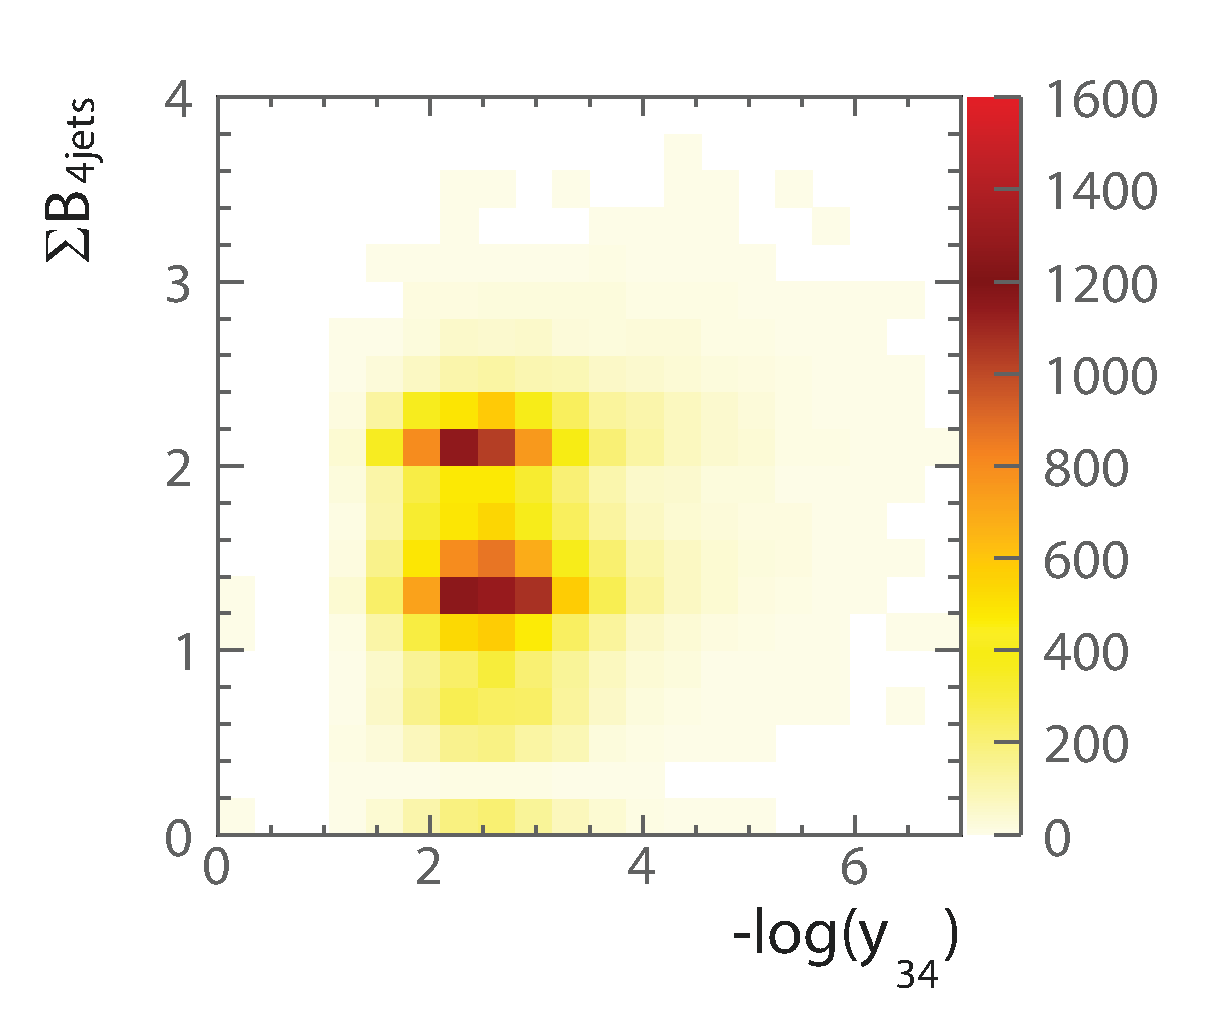
\includegraphics[width=\textwidth]{{doubleHiggs/preSel/mutual6025bbWW2}}
    \caption{\eeToHHbbWW, hadronic}
    \label{fig:doubleHiggs3MutualbbWW}
  \end{subfigure}
    \begin{subfigure}[b]{0.45\textwidth}
    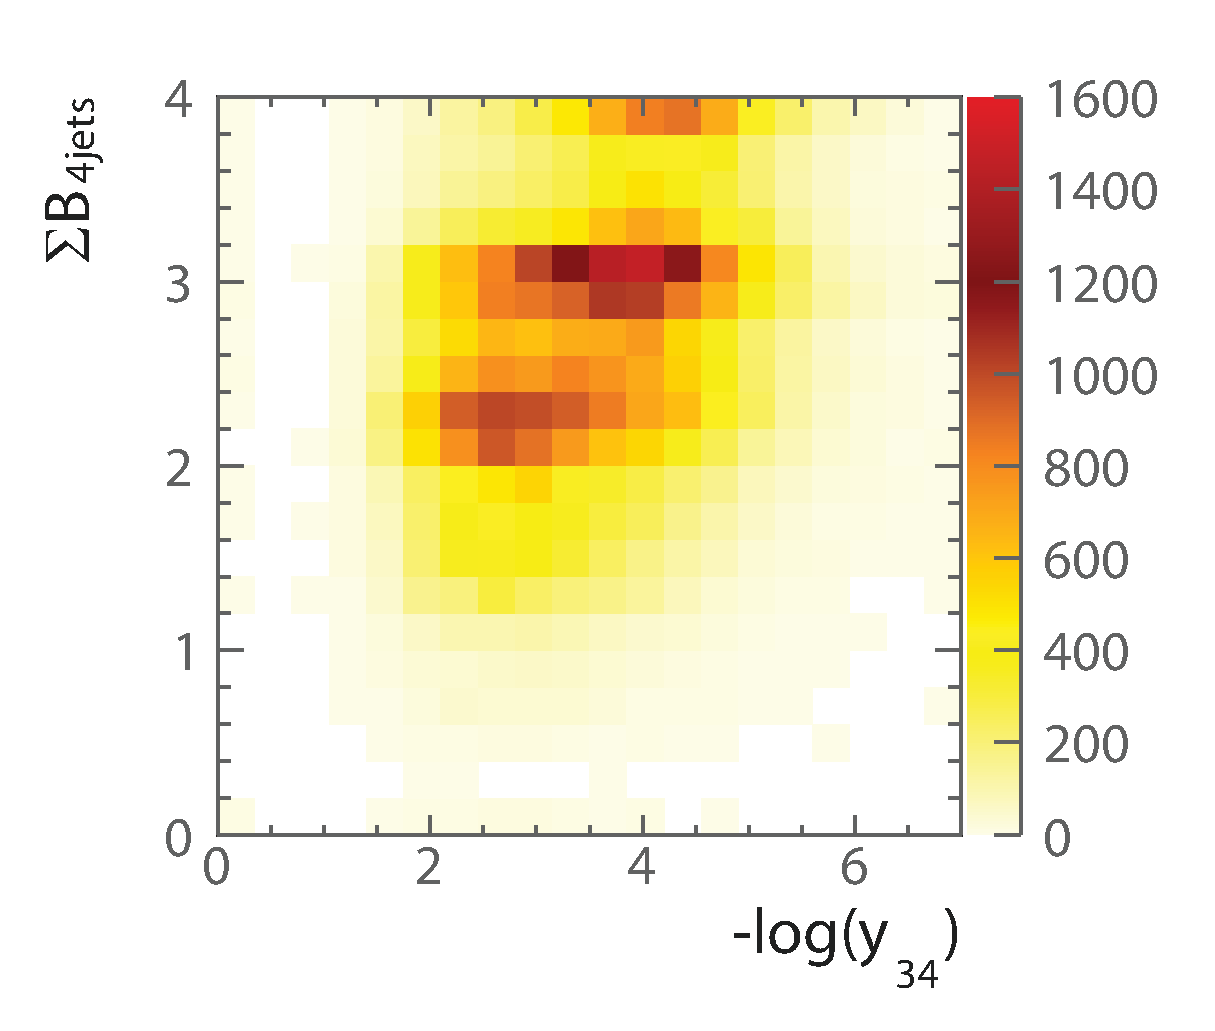
\includegraphics[width=\textwidth]{{doubleHiggs/preSel/mutual6025bbbb2}}
    \caption{\eeToHHbbbb}
    \label{fig:doubleHiggs3Mutualbbbb}
  \end{subfigure}
\caption[Sum of b-jet tag as a function of \y{34} at \rootS{3}]%
   {The two-dimensional distributions of sum of b-jet tag values against $-\log\parenths{\y{34}}$ for: a)  hadronic \WW decay of \eeToHHbbWW; and b) \eeToHHbbbb events at \rootS{3}. The sum of b-jet tag values is calculated for the cases where events are clustered into four jets.}
   \label{fig:doubleHiggs3TeVMutualPreselection}
\end{figure}

The pre-selection cuts at \rootS{3} use the same cut on $m_{\HH}$. The cut on  b-jet tag is different because the performance of flavour tagging is worse at \rootS{3} in comparison to the performance at \rootS{1.4}. \FIGURE{fig:doubleHiggs3PreSelbtag} shows the distribution of the highest b-jet tag value, where the cut above 0.7 helps to reduce background events with no \Pbottom quarks in final states.  \FIGURE{fig:doubleHiggs3PreSelmHH} shows the distribution of the invariant mass of the two Higgs system, where the cut above 150\,GeV is effective against samples with two-quark final states.  The fractions of events passing each pre-section cut for individual processes are listed in  \Table{tab:doubleHiggs3TeVPreslectionPart2}.


\begin{figure}[!htbp]
    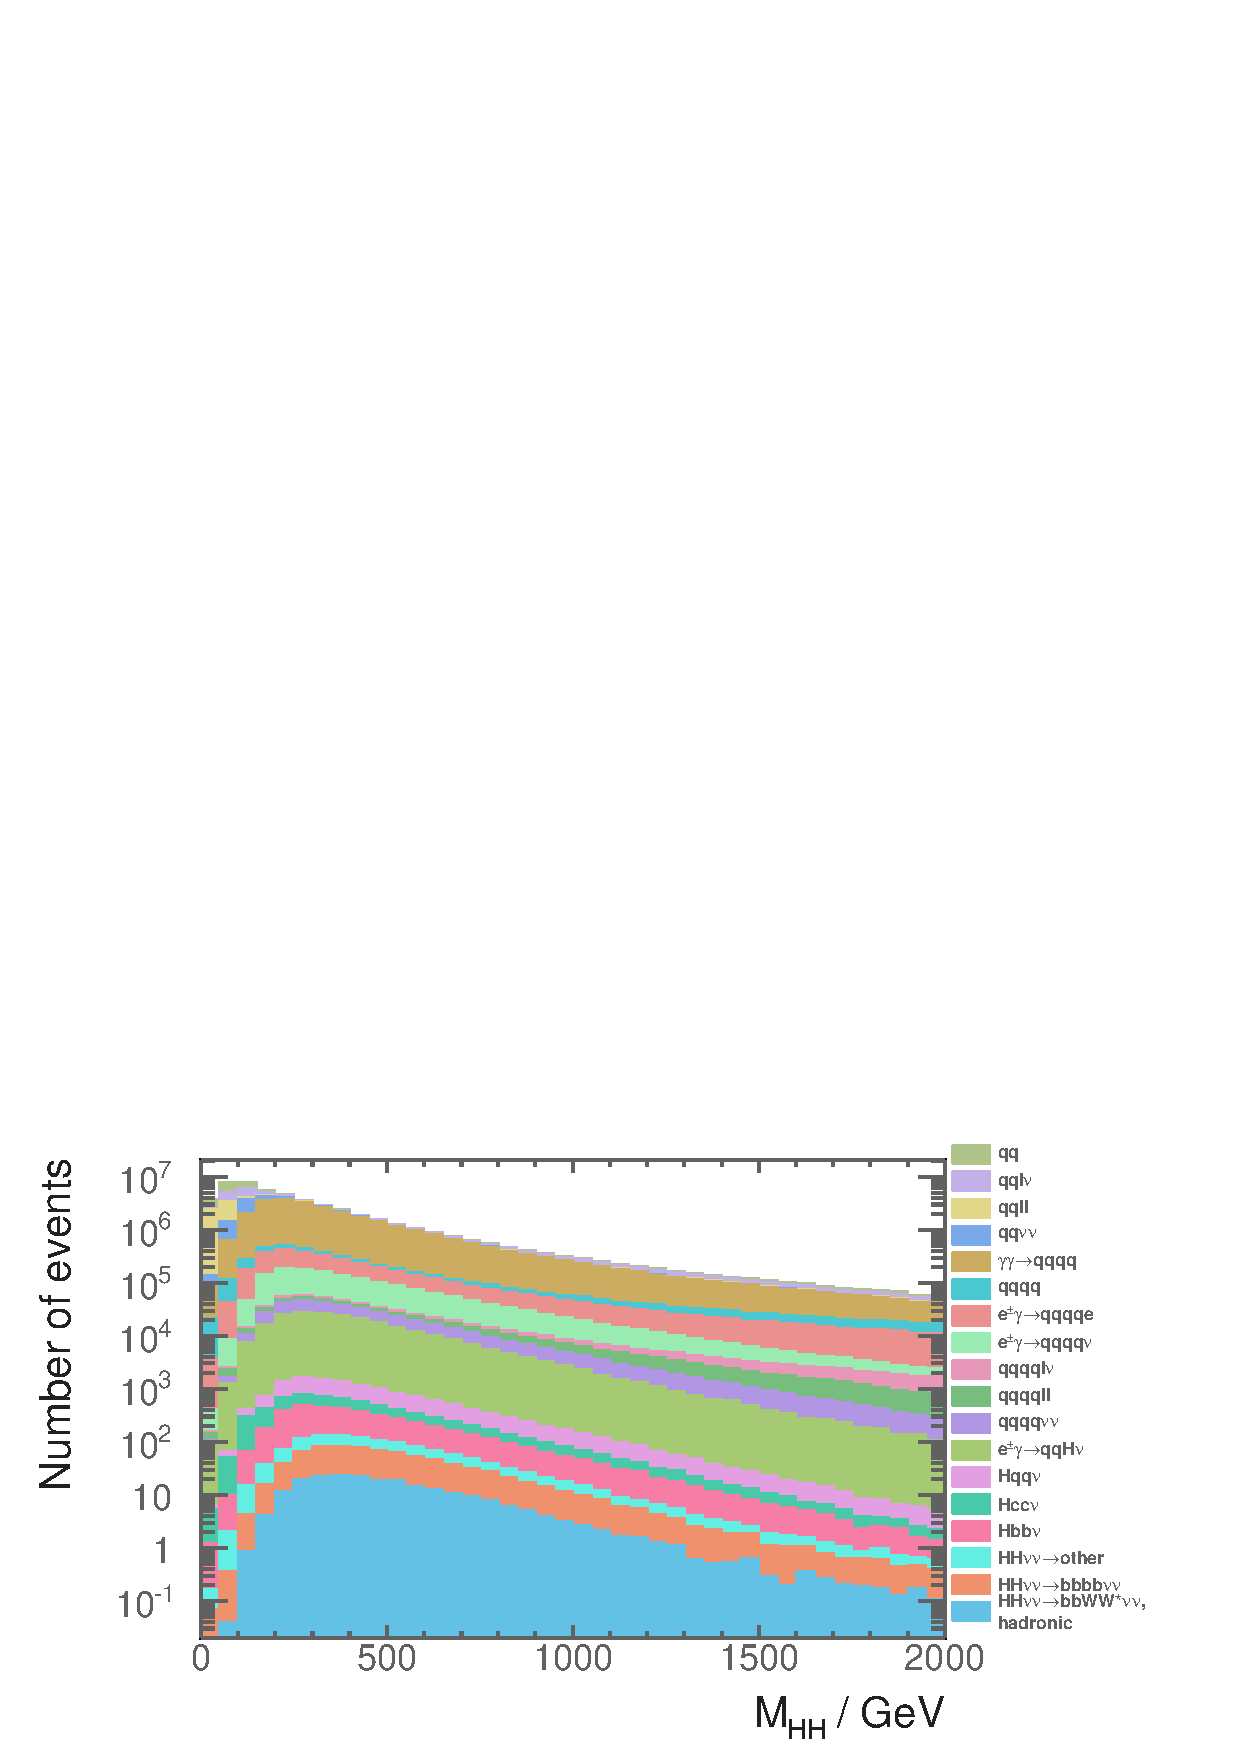
\includegraphics[width=0.95\textwidth]{{doubleHiggs/preSel2/tR0_7_6jet_btag2_Higgs_all_M_TMVA201612083TeVtR0_7_qq_btag2_prepare}.pdf}
    \caption{Distributions of the invariant mass  of the two Higgs system for \rootS{3}, assuming an integrated luminosity of 2000\,\uprightMath{fb^{-1}}.}
    \label{fig:doubleHiggs3PreSelmHH}
\end{figure}

\begin{figure}[!htbp]
    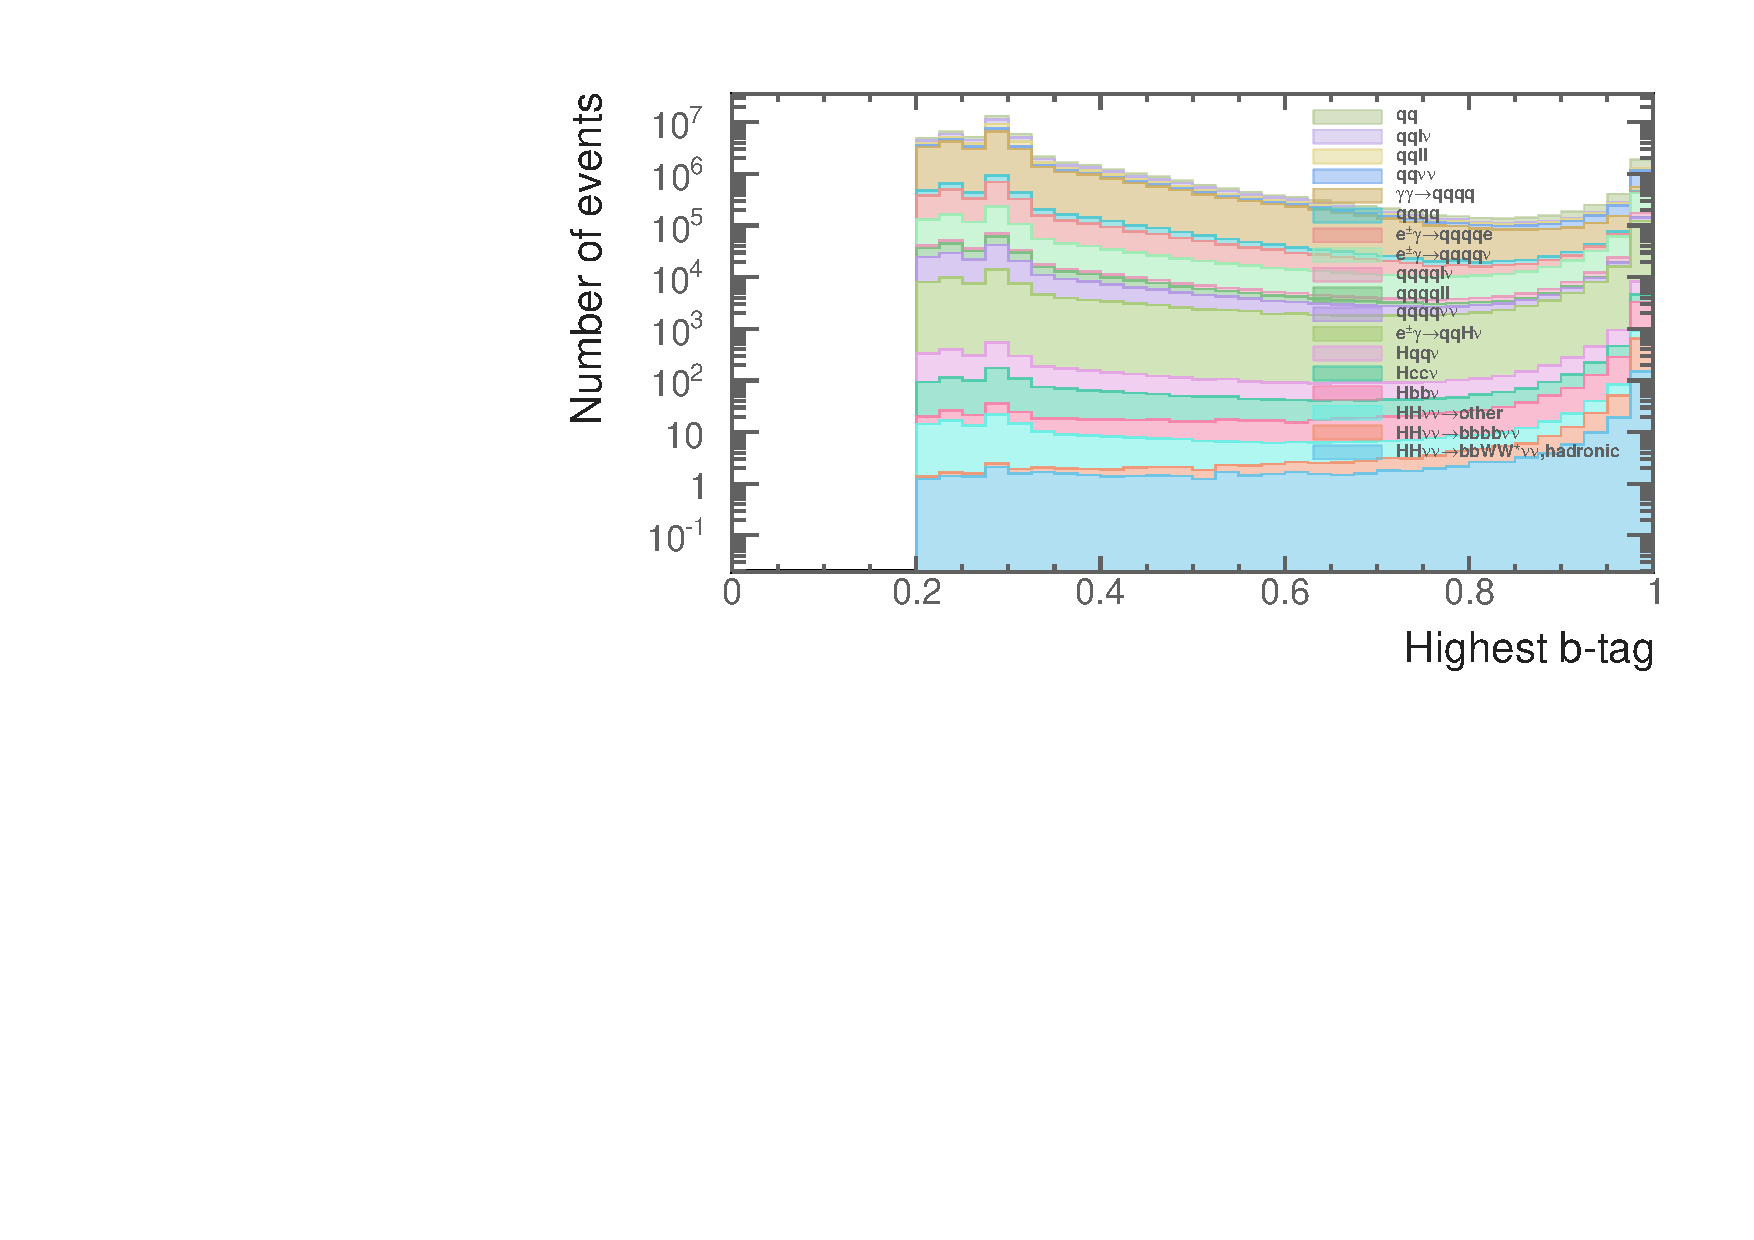
\includegraphics[width=0.95\textwidth]{{doubleHiggs/preSel2/tR0_7_6jet_btag2_bTag1_TMVA201612083TeVtR0_7_qq_btag2_prepare}.pdf}
    \caption{Distributions of the highest b-jet tag value for \rootS{3}, assuming an integrated luminosity of 2000\,\uprightMath{fb^{-1}}.}
    \label{fig:doubleHiggs3PreSelbtag}
\end{figure}

The cuts to aid the MVA at \rootS{3} are largely the same as the ones at \rootS{1.4}, apart from the difference on the cut of the invariant mass of double Higgs system due to a higher centre-of-mass energy. The cuts are the invariant mass of the \Hbb < 500\,GeV, the invariant mass of the \HWW < 800\,GeV, the invariant mass of the \PW < 200\,GeV, and the invariant mass of the double Higgs system < 3000\,GeV.


\begin{comment}
\begin{table}[!htbp]
\begin{tabular}{lrr}
\hline
\hline
Processor / Efficiency (3\,TeV)  &  Signal  & \egamma{\Pem}{\Pphoton}{BS}{\Pem \Pquark \Pquark \Pquark \Pquark}  \\
\hline
Combined light lepton finder & 84.4\% & 72.7\%  \\
ForwardFinderProcessor & 95.9\% & 55.4\%  \\
Combined & 81.0\% &  33.4\%  \\
\hline
\hline

\end{tabular}
\caption{Very forward electron and photon finder performance on the signal and selected background samples.}
\label{tab:doubleHiggs3TeVForwardPerformance}
\end{table}
\end{comment}


% The optimal "what?" chosen is tight tightPFO?

\begin{comment}
\begin{table}[!htbp]
\begin{tabular}{lrr}
\hline
\hline
Jet Parameters  & \rootS{3}  \\
\hline
$\mu_{\Hbb}$  & $119.1_{\pm0.3}$  \\
$\sigma_{L,\Hbb}$ & $15.0_{\pm0.3}$  \\
$\sigma_{R,\Hbb}$ & $8.4_{\pm0.2}$  \\
\hline
$\mu_{\HWW}$ &  $123.0_{\pm0.3}$  \\
$\sigma_{L,\HWW}$ & $36.6_{\pm0.6}$  \\
$\sigma_{R,\HWW}$ & $7.4_{\pm0.2}$  \\
\hline
$\mu_{\PW}$  & $78.1_{\pm0.3}$ \\
$\sigma_{L,\PW}$ & $13.1_{\pm0.4}$  \\
$\sigma_{R,\PW}$ &  $9.5_{\pm0.2}$  \\
\hline
\hline
\end{tabular}
\caption
[The extracted fitted parameters of optimal jet reconstructions at \rootS{3}.] %
{The extracted fitted parameters of optimal jet reconstructions for \tightPFO with $R = 0.7$ at \rootS{3}.}
\label{tab:doubleHiggs3TeVFitParameters}
\end{table}
\end{comment}


%why have the pre-selection cuts changed?

%The cut is aggressive to compensate for the worse performance of the flavour tagging at high \sqrtS.

\begin{comment}

\begin{table}[!htbp]
\begin{tabular}{lr}
\hline
\hline
Pre-selection  &  \rootS{3}  \\
\hline
Discriminative pre-selection & \multicolumn{1}{R{0.5\textwidth}}{$m_{\HH} > 150\,GeV$, $B_1 > 0.7$,  $\pT_{\HH} > 30\,GeV$} \\
Loose cuts for MVA &  \multicolumn{1}{R{0.5\textwidth}}{$m_{\Hbb} < 500\,GeV$, $m_{\HWW} < 800\,GeV$, $m_{\PW} < 200\,GeV$, $m_{\HH} <3000\,GeV$} \\
Mutually exclusive & \sumBtag{4} < 2.3, \y{34} < 3.6 \\
\hline
\hline
\end{tabular}
\caption
{Pre-selection cuts at \rootS{3}.}
\label{tab:doubleHiggs3TeVPreSel}
\end{table}
\end{comment}
% The cut on $m_{HH}$ is effective against background with fewer number of quarks in the final states. The cut on $B_1$ is effective against final states with no b quark.





\begin{comment}
\begin{table}\centering
\begin{tabular}{llrr}
\hline
\hline
\sqrtS & $selection$ & \multicolumn{1}{m{4cm}}{\eeToHHbbqqqq Selection Efficiency} & \multicolumn{1}{m{4cm}}{\eeToHHbbbb Selection Efficiency} \\
1.4\,TeV &  \sumBtag{4} < 2.3 and \y{34} < 3.7 & 86\% & 78\% \\
3\,TeV &  \sumBtag{4} < 2.3 and \y{34} < 3.6 & 89\% & 82\% \\
\hline
\hline
\end{tabular}
\caption[Mutually exclusive cuts] %
{Mutually exclusive cuts, for full signal samples}
\label{tab:doubleHiggsMutualCuts}
\end{table}
\end{comment}

The same set of variables are used in the MVA as in the analysis at \rootS{1.4}. The optimised parameters of the Boosted Decision Tree classifier are the same. The efficiencies of the MVA event selection and the numbers of events after the MVA event selection are listed in \Table{tab:doubleHiggs3TeVMVA}. Background processes that are dominant after the MVA event selection are almost identical to those at \rootS{1.4}. Hence see \Section{sec:doubleHiggsSignalSelResult} for discussion.

\begin{table}[!htbp]\centering
%\small{
\small
\begin{tabular}{lrrrr}
\hline \hline
 \multicolumn{1}{m{3.5cm}}{\rootS{3}} &  \multicolumn{1}{R{2cm}}{N}  & \multicolumn{1}{R{2cm}}{$\varepsilon_{presel}$} & \multicolumn{1}{R{2cm}}{$\varepsilon_{MVA}$} & \multicolumn{1}{R{2cm}}{$N_{MVA}$} \\

\hline
\eeToHH $\to$ \\
\HepProcess{ \Pbottom \APbottom \PWplus \PWminus \Pnue \APnue}, hadronic             &146.0& 61.7\% & 11.6\% & 9.89\\
\hline
\eeToHH $\to$ \\
\HepProcess{ \Pbottom \APbottom \Pbottom \APbottom \Pnue \APnue}             &355.0& 18.8\% & 1.5\% & 1.05 \\
\eeToHH $\to$ other                             & 675.0 & 20.0\% & 3.6\% & 4.51 \\
\hline
\eeTo{\qlight \qlight \PHiggs \Pnu \APnu}  & 6120 & 36.0\% & 0.4\% & 9.42\\
\eeTo{\Pcharm \APcharm \PHiggs \Pnu \APnu}  & 2300 & 26.3\%& 0.5\%& 3.13\\
\eeTo{\Pbottom \APbottom \PHiggs \Pnu \APnu}  & 3560 & 25.8\%& 1.2\%& 6.82\\

\eeTo{ \Pquark \Pquark \Pquark \Pquark}   &   1093000& 1.4\% & 0.01\%& 1.43\\
\eeTo{ \Pquark \Pquark \Pquark \Pquark \Plepton \Plepton}& 338600 & 0.6\%&  - & -\\
\eeTo{ \Pquark \Pquark \Pquark \Pquark \Plepton \Pnu}& 213200 & 7.3\%& 0.05\%& 8.35\\
\eeTo{ \Pquark \Pquark \Pquark \Pquark \Pnu \APnu} & 143000& 9.0\%& 0.05\%& 6.35\\

\eeTo{ \Pquark \Pquark} &  5897800 & 1.4\%&  - & - \\
\eeTo{ \Pquark \Pquark \Plepton \Pnu} &  11121800 & 0.1\%& - & - \\
\eeTo{ \Pquark \Pquark \Pl \Pl} &  6639200 & 0.4\%& - & - \\
\eeTo{ \Pquark \Pquark \Pnu \Pnu} & 2635000 & 3.1\%&  - & - \\
\hline
\egamma{\Pepm}{\Pphoton}{\BS}{\Pepm \Pquark \Pquark \Pquark \Pquark} & 4007354  & 0.7\%&  - & - \\
%\egamma{\Pem}{\Pphoton}{BS}{\Pem \Pquark \Pquark \Pquark \Pquark} & 2004388.1  & 0.7\%&  - & - \\
%\egamma{\Pep}{\Pphoton}{BS}{\Pep \Pquark \Pquark \Pquark \Pquark} & 2002334.1 & 0.7\%&  - & - \\
\egamma{\Pepm}{\Pphoton}{\EPA}{\Pepm \Pquark \Pquark \Pquark \Pquark} & 1151200& 0.4\%&  - & - \\
%\egamma{\Pem}{\Pphoton}{EPA}{\Pem \Pquark \Pquark \Pquark \Pquark} & 575600.0& 0.4\%&  - & - \\
%\egamma{\Pep}{\Pphoton}{EPA}{\Pep \Pquark \Pquark \Pquark \Pquark}  & 575600.0 & 0.3\% &  - & - \\
\egamma{\Pepm}{\Pphoton}{\BS}{\Pnu \Pquark \Pquark \Pquark \Pquark}& 829184  & 16.4\%& 0.04\%& 61.0\\
%\egamma{\Pem}{\Pphoton}{BS}{\Pnu \Pquark \Pquark \Pquark \Pquark}& 414750.0  & 16.8\%& 0.04\%& 30.7\\
%\egamma{\Pep}{\Pphoton}{BS}{\APnu \Pquark \Pquark \Pquark \Pquark}& 414434.0 & 15.9\% & 0.05\%& 30.3\\
\egamma{\Pepm}{\Pphoton}{\EPA}{\Pnu \Pquark \Pquark \Pquark \Pquark}& 216800  & 7.6\% & 0.04\%& 6.0\\
%\egamma{\Pem}{\Pphoton}{EPA}{\Pnu \Pquark \Pquark \Pquark \Pquark}& 108400.0  & 7.8\% & 0.04\%& 3.37\\
%\egamma{\Pep}{\Pphoton}{EPA}{\APnu \Pquark \Pquark \Pquark \Pquark}& 108400.0  & 7.3\%& 0.03\%& 2.63 \\
\egamma{\Pepm}{\Pphoton}{\BS}{\Pquark \Pquark \PHiggs \Pnu} & 185018  & 30.2\% & 0.2\%& 121.7 \\
%\egamma{\Pem}{\Pphoton}{BS}{\Pquark \Pquark \PHiggs \Pnu} & 92588.0  & 30.2\% & 0.2\%& 67.5 \\
%\egamma{\Pep}{\Pphoton}{BS}{\Pquark \Pquark \PHiggs \Pnu} & 92430.0 & 30.3\% & 0.2\% & 54.2 \\
\egamma{\Pepm}{\Pphoton}{\EPA}{\Pquark \Pquark \PHiggs \Pnu} & 46800.0 & 15.3\% & 0.2\% & 18.1 \\
%\egamma{\Pem}{\Pphoton}{EPA}{\Pquark \Pquark \PHiggs \Pnu} & 23400.0 & 15.4\% & 0.2\% & 7.88 \\
%\egamma{\Pep}{\Pphoton}{EPA}{\Pquark \Pquark \PHiggs \Pnu} & 23400.0   & 15.2\% & 0.3\% & 10.2 \\
\hline
\gammagamma{\Pphoton}{\BS}{\Pphoton}{\BS}{ \Pquark \Pquark \Pquark \Pquark}& 18009414  & 1.6\%&   - & - \\
\gammagamma{\Pphoton}{\BS}{\Pphoton}{\EPA}{ \Pquark \Pquark \Pquark \Pquark}& 3824548  & 1.0\%&  - & - \\
\gammagamma{\Pphoton}{\EPA}{\Pphoton}{\BS}{ \Pquark \Pquark \Pquark \Pquark}& 3828498& 1.0\%&  - & - \\
\gammagamma{\Pphoton}{\EPA}{\Pphoton}{\EPA}{ \Pquark \Pquark \Pquark \Pquark}& 805400 & 0.6\%&  - & - \\
\hline \hline
\end{tabular}
\caption[List of signal and background selection efficiencies and event numbers after MVA application at  \rootS{3}.]
{List of signal and background events with selection efficiency and number of events at \rootS{3}, assuming an integrated  luminosity of 2000\,\uprightMath{fb^{-1}}. The number of events ($N$), the selection efficiencies of pre-selection cuts ($\varepsilon_{presel}$), the selection efficiencies of the MVA event selection after pre-selection cuts ($\varepsilon_{MVA}$), and the number of events after the MVA event selection ($N_{MVA}$) are shown. The entries marked with ``-'' represent  numbers less than 0.01. \Pquark can be \Pup, \Pdown, \Pstrange, \Pbottom or \Ptop. Unless specified, \Pquark, \Plepton and \Pnu represent either particles or the corresponding anti-particles.}
\label{tab:doubleHiggs3TeVMVA}
\end{table}

\section{Semi-leptonic decay at \rootS{3} analysis}

The final analysis is the semi-leptonic \WW decay of \eeToHH $\to$ \HepProcess{ \Pbottom \APbottom \PWplus \PWminus \Pnu \APnu}  at \rootS{3}. The semi-leptonic decay analysis at \rootS{1.4} was also performed. However there are not enough signal events to have a meaningful discussion for the analysis at \rootS{1.4}. Hence, only the semi-leptonic decay analysis at \rootS{3} is presented.

The strategy of the semi-leptonic decay  analysis is very similar to the hadronic decay analysis. The main differences are that there is one lepton in the final state and the final state has four quarks instead of six. \Hbb and \PW can not be reconstructed due to the leptonic decay of one of the \PW{s}. Hence, the signal events are selected when there is one identified lepton using the same lepton finding processors. The jet reconstruction parameters are the same as hadronic decay analysis at the \rootS{3}. There are no mutually exclusive cuts since there is no semi-leptonic analysis for the \eeToHHbbbb sub-channel.

The pre-selection cuts are similar to the cuts in the hadronic analysis. The invariant mass of the double Higgs system is required to be above 150\,GeV. The highest b-jet tag value is higher than 0.2. The transverse momentum of the double Higgs system is higher than 30\,GeV.

Variables used in the MVA classifier, listed in  \Table{tab:doubleHiggsVaraiblesSemiLep},  belong to  a reduced set of the variables  used in the hadronic decay analysis, as \HWW and one \PW can not be reconstructed in the semi-hadronic decay analysis. For the same reason, the cuts to aid the MVA are reduced to the invariant mass of \Hbb < 500\,GeV and the invariant mass of the double Higgs system < 3000\,GeV.



\TABLE{tab:doubleHiggsQlv3TeVMVA} lists the  selection efficiency and number of events after the MVA event selection for individual processes at \rootS{3}, assuming an integrated luminosity of 2000\,\uprightMath{fb^{-1}}.  Almost all background processes are non-zero after the MVA event selection. Nevertheless,  dominant background processes are almost identical to the hadronic decay analysis  at \rootS{3}. Hence discussion of the MVA event selection is provided in \Section{sec:doubleHiggsSignalSelResult}.
%"dominant background channels"?
\begin{comment}
\begin{table}[!htbp]
\begin{tabular}{lr}
\hline
\hline
Pre-selection  &  \rootS{3}  \\
\hline
Discriminative pre-selection & \multicolumn{1}{R{0.5\textwidth}}{$m_{\HH} > 150\,GeV$, $B_1 > 0.2$,  $\pT_{\HH} > 30\,GeV$} \\
Loose cuts for MVA &  \multicolumn{1}{R{0.5\textwidth}}{$m_{\Hbb} < 500\,GeV$, $m_{\HH} <3000\,GeV$} \\
\hline
\hline
\end{tabular}
\caption
{Pre-selection cuts at \rootS{3} for semi-leptonic analysis.}
\label{tab:doubleHiggs3TeVPreSelSemiLep}
\end{table}
\end{comment}

 \begin{table}[!htbp]\centering
\begin{tabular}{lr}
\hline
\hline
Category &  Variable \\
\hline
Invariant mass &  \multicolumn{1}{R{0.6\textwidth}}{$m_{\Hbb}$, $m_{\PW}$, $m_{\HH}$} \\
Energy and momentum & \multicolumn{1}{R{0.6\textwidth}}{$E_{mis}$, $\pT_{\Hbb}$, $\pT_{\PW}$, $\pT_{\HH}$} \\
Lab-frame angles & \multicolumn{1}{R{0.6\textwidth}}{$\theta_{mis}$, $\acolinearity{\Hbb}$, $\acolinearity{\PW}$, $\acolinearity{\HH}$} \\
Boosted-frame frames & \multicolumn{1}{R{0.6\textwidth}}{$\cosStar{\Hbb}$, $\cosStar{\HH}$} \\
Event shape & \multicolumn{1}{R{0.6\textwidth}}{$\abs{\sphericity}$, $-\ln(\y{23})$, $-\ln(\y{34})$, $-\ln(\y{45})$, $-\ln(\y{56})$} \\
\Pbottom and \Pcharm tag & \multicolumn{1}{R{0.6\textwidth}}{$\btagFull{1}{\Hbb}$, $\btagFull{2}{\Hbb}$, $\btagFull{1}{\PW}$, $\ctagFull{1}{\Hbb}$, $\ctagFull{1}{\PW}$} \\
Particle number &  \multicolumn{1}{R{0.6\textwidth}}{$\npfo{\Hbb}$, $\npfo{\PW}$} \\
\hline
\hline
\end{tabular}
\caption
{Variables used in the MVA event selection for the semi-leptonic \WW decay of \eeToHHbbWW analysis  at \rootS{3}.}
\label{tab:doubleHiggsVaraiblesSemiLep}
\end{table}





\begin{table}[!htbp]\centering
%\small{

\begin{tabular}{lrrrr}
\hline \hline
 \multicolumn{1}{m{3.5cm}}{\rootS{3}} &  \multicolumn{1}{R{2cm}}{N}  & \multicolumn{1}{R{2cm}}{$\varepsilon_{presel}$} & \multicolumn{1}{R{2cm}}{$\varepsilon_{MVA}$} & \multicolumn{1}{R{2cm}}{$N_{MVA}$} \\
\hline
\eeToHH $\to$ \\
\HepProcess{ \Pbottom \APbottom \PWplus \PWminus \Pnue \APnue}, semi-leptonic       &96.8& 44.6\% & 21.9\% & 13.11\\
\hline
\eeToHH $\to$ \\
\HepProcess{ \Pbottom \APbottom \Pbottom \APbottom \Pnue \APnue}             &355.0& 13.3\% & 10.9\% &  5.38\\
\eeToHH $\to$ other                             & 724.2 & 13.1\% & 13.6\% &  12.75\\
\hline
\eeTo{\qlight \qlight \PHiggs \Pnu \APnu}  & 6120 & 7.4\% & 13.7\% & 62.63\\
\eeTo{\Pcharm \APcharm \PHiggs \Pnu \APnu}  & 2300 & 6.3\%& 12.1\%& 17.10\\
\eeTo{\Pbottom \APbottom \PHiggs \Pnu \APnu}  & 3560 & 15.9\%& 5.1\%& 18.03\\

\eeTo{ \Pquark \Pquark \Pquark \Pquark}   &   1093000& 0.6\% & 0.2\%& 15.04\\
\eeTo{ \Pquark \Pquark \Pquark \Pquark \Plepton \Plepton}& 338600 & 1.0\%&  0.06\% & 1.85\\
\eeTo{ \Pquark \Pquark \Pquark \Pquark \Plepton \Pnu}& 213200 & 27.6\%& 0.5\%& 270.33\\
\eeTo{ \Pquark \Pquark \Pquark \Pquark \Pnu \APnu} & 143000& 1.9\%& 1.6\%& 43.78\\

\eeTo{ \Pquark \Pquark} &  5897800 & 0.4\%&  0.3\% & 60.82 \\
\eeTo{ \Pquark \Pquark \Plepton \Pnu} &  11121800 & 0.3\%& 0.08\% & 21.24 \\
\eeTo{ \Pquark \Pquark \Pl \Pl} &  6639200 & 0.6\%& 0.2\%& 84.14\\
\eeTo{ \Pquark \Pquark \Pnu \Pnu} & 2635000 & 0.4\%&  0.9\% & 92.55 \\
\hline
\egamma{\Pepm}{\Pphoton}{\BS}{\Pepm \Pquark \Pquark \Pquark \Pquark} & 4007354  & 1.2\%&  - & - \\
%\egamma{\Pem}{\Pphoton}{BS}{\Pem \Pquark \Pquark \Pquark \Pquark} & 2004388.1  & 1.2\%&  - & - \\
%\egamma{\Pep}{\Pphoton}{BS}{\Pep \Pquark \Pquark \Pquark \Pquark} & 2002334.1 & 1.2\%&  - & - \\
\egamma{\Pepm}{\Pphoton}{\EPA}{\Pepm \Pquark \Pquark \Pquark \Pquark} & 1151200& 1.1\%&  - & - \\
%\egamma{\Pem}{\Pphoton}{EPA}{\Pem \Pquark \Pquark \Pquark \Pquark} & 575600.0& 1.1\%&  - & - \\
%\egamma{\Pep}{\Pphoton}{EPA}{\Pep \Pquark \Pquark \Pquark \Pquark}  & 575600.0 & 1.1\% &  - & - \\
\egamma{\Pepm}{\Pphoton}{\BS}{\Pnu \Pquark \Pquark \Pquark \Pquark}& 829184  & 3.6\%& 1.5\%& 452.45\\
%\egamma{\Pem}{\Pphoton}{BS}{\Pnu \Pquark \Pquark \Pquark \Pquark}& 414750.0  & 3.7\%& 1.5\%& 226.77\\
%\egamma{\Pep}{\Pphoton}{BS}{\APnu \Pquark \Pquark \Pquark \Pquark}& 414434.0 & 3.5\% & 1.6\%& 225.68\\
\egamma{\Pepm}{\Pphoton}{\EPA}{\Pnu \Pquark \Pquark \Pquark \Pquark}& 216800  & 11.0\% & 0.9\%& 200.65\\
%\egamma{\Pem}{\Pphoton}{EPA}{\Pnu \Pquark \Pquark \Pquark \Pquark}& 108400.0  & 11.2\% & 0.9\%& 107.90\\
%\egamma{\Pep}{\Pphoton}{EPA}{\APnu \Pquark \Pquark \Pquark \Pquark}& 108400.0  & 10.7\%& 0.8\%& 92.75 \\
\egamma{\Pepm}{\Pphoton}{\BS}{\Pquark \Pquark \PHiggs \Pnu} & 185018  & 7.9\% & 10.4\%& 1521.93 \\
%\egamma{\Pem}{\Pphoton}{BS}{\Pquark \Pquark \PHiggs \Pnu} & 92588.0  & 7.9\% & 10.7\%& 779.36 \\
%\egamma{\Pep}{\Pphoton}{BS}{\Pquark \Pquark \PHiggs \Pnu} & 92430.0 & 7.9\% & 10.1\% & 741.57 \\
\egamma{\Pem}{\Pphoton}{\EPA}{\Pquark \Pquark \PHiggs \Pnu} & 46800 & 22.8\% & 7.1\% & 750.85 \\
%\egamma{\Pem}{\Pphoton}{EPA}{\Pquark \Pquark \PHiggs \Pnu} & 23400.0 & 22.9\% & 6.9\% & 369.52 \\
%\egamma{\Pep}{\Pphoton}{EPA}{\Pquark \Pquark \PHiggs \Pnu} & 23400.0   & 22.7\% & 7.2\% & 381.33 \\
\hline
\gammagamma{\Pphoton}{\BS}{\Pphoton}{\BS}{ \Pquark \Pquark \Pquark \Pquark}& 18009414  & 0.4\%&   - & - \\
\gammagamma{\Pphoton}{\BS}{\Pphoton}{\EPA}{ \Pquark \Pquark \Pquark \Pquark}& 3824548 & 1.0\%&  - & - \\
\gammagamma{\Pphoton}{\EPA}{\Pphoton}{\BS}{ \Pquark \Pquark \Pquark \Pquark}& 3828498 & 1.0\%&  0.08\% & 28.85 \\
\gammagamma{\Pphoton}{\EPA}{\Pphoton}{\EPA}{ \Pquark \Pquark \Pquark \Pquark}& 805400& 1.1\%&  - & - \\
\hline \hline
\end{tabular}
\caption
{List of signal and background events with selection efficiency and number of events at \rootS{3}  for semi-leptonic \WW decay of \eeToHHbbWW analysis, assuming an integrated luminosity of 2000\,\uprightMath{fb^{-1}}. The number of events ($N$), the selection efficiencies of pre-selection cuts ($\varepsilon_{presel}$), the selection efficiencies of MVA after pre-selection cuts ($\varepsilon_{MVA}$), and the number of events after MVA ($N_{MVA}$) are shown. The entries marked with ``-'' represent  numbers less than 0.01. \Pquark can be \Pup, \Pdown, \Pstrange, \Pbottom or \Ptop. Unless specified, \Pquark, \Plepton and \Pnu represent either particles or the corresponding anti-particles.}
\label{tab:doubleHiggsQlv3TeVMVA}
\end{table}
%semi-leptonic \WW decay of \eeToHHbbWW
\section{Result interpretation}
\label{sec:doubleHiggsResults}



The numbers of signal events and background events and significance after the MVA event selection for analyses at the \rootS{1.4} and \rootS{3}  are listed in \Table{tab:doubleHiggsResult}. The significance is defined as the number of signal events divided by the square root of the sum of  the signal and background events. The \ee collision at \rootS{1.4} assumes an integrated luminosity of 1500\,\uprightMath{fb^{-1}}, whilst that of the \rootS{3} assumes an integrated luminosity of 2000\,\uprightMath{fb^{-1}}.  For the hadronic \WW decay of \eeToHHbbWW analysis at \rootS{1.4}, the numbers of signal and background events after the MVA selection are 1.79 and 8.41 respectively. For the hadronic analysis at \rootS{3}, the respective numbers of the signal and background events after the MVA selection are 15.45 and 242.28. For the semi-leptonic \WW decay of \eeToHHbbWW analysis at \rootS{3}, the numbers of the signal and background events after the MVA selection are 31.24 and 3612.39 respectively.

 %and \rootS{3}, numbers of the signal events passing the MVA event selection are 1.79 and 15.45, respectively, and the numbers of background events passing the MVA event selection are 8.41 and 242.28, respectively. For  the semi-leptonic \WW decay of \eeToHHbbWW analyses \rootS{3}, the number of the signal events passing the MVA event selection is 31.24, whilst the  numbers of background events passing the MVA event selection is 3612.39.

% which is roughly $\sqrt{N_S + N_B} / N_S$ at \rootS{1.4} and 3\,TeV,

\begin{table}[!htbp]
\begin{tabular}{lrrr}
\hline
\hline
Process  &  $N_{S}$ & $N_{B}$ & $\frac{N_S} { \sqrt{N_S + N_B}}$ \\
\hline
\multicolumn{1}{L{0.3\textwidth}}{\eeToHHbbWW, hadronic, \rootS{1.4}} & 1.79 & 8.41 & 0.56 \\
\multicolumn{1}{L{0.3\textwidth}}{\eeToHHbbWW, hadronic, \rootS{3}} & 15.45 & 242.28 & 0.96 \\
\multicolumn{1}{L{0.3\textwidth}}{\eeToHHbbWW, semi-leptonic, \rootS{3}} &  31.24& 3612.39 & 0.52 \\
\hline
\hline
\end{tabular}
\caption
{Number of signal ($N_S$) and background  ($N_B$) events, and significance ($N_S / \sqrt{N_S + N_B}$) after MVA event selections for \eeToHHbbWW analyses at \rootS{1.4} and 3\,TeV. The \ee collision at \rootS{1.4} assumes an integrated luminosity of 1500\,\uprightMath{fb^{-1}}, whilst that of \rootS{3} assumes an integrated luminosity of 2000\,\uprightMath{fb^{-1}}.}
\label{tab:doubleHiggsResult}
\end{table}


The expected uncertainties on the measurement of the double Higgs production cross sections are estimated to be the inverse of the significance \cite{Agashe:2014kda}:
\begin{equation}
\frac{\Delta\left[\sigma\left(\HHvv\right)\right]}{\sigma\left(\HHvv\right)} =
\begin{cases}
  179\%, & \mbox{at \rootS{1.4}, }  \\
  92\%, & \mbox{at \rootS{3}}.
\end{cases}
\end{equation}
%where $N_S$ is the number of  \eeToHH events passing the MVA event selection and $N_B$ is the number of background events passing the MVA event selection.

The expected uncertainty at \rootS{3} combines the results from analyses for the hadronic and semi-leptonic decay sub-channels.


%. The relative uncertainty on the \gHHH coupling can be related to the uncertainty on the cross section
The Higgs trilinear self coupling \gHHH is related to the double Higgs production cross section via  \cite{Abramowicz:2016zbo}:
\begin{equation}
\frac{\Delta\gHHH}{\gHHH}\approx \kappa \cdot \frac{\Delta\left[\sigma\left(\HHvv\right)\right]}{\sigma\left(\HHvv\right)},
\label{eqn:doubleHiggs1Dextration}
\end{equation}
The coefficient $\kappa$ can be determined by parameterising the \eeToHH cross section as a function of the coupling \gHHH. \FIGURE{fig:doubleHiggsCouplingOneDRelation} shows the \eeToHH cross sections as a function of the coupling \gHHH for \rootS{1.4} and \rootS{3}. At the SM \gHHH value, the coefficient $\kappa$ is 1.22 at \rootS{1.4}, and 1.47  at  \rootS{3}.

%The negative gradient indicates that for all processes producing double Higgs, the process  that is  sensitive to the \gHHH experiences destructive interferences with other SM processes with the same final state.
%Since $\kappa$ is extracted from the relation at generator level, the fully simulated reconstruction selection may favour certain Feynman diagrams, therefore affecting the sensitivity to $\lambda$ .


\begin{figure}[!htbp]
    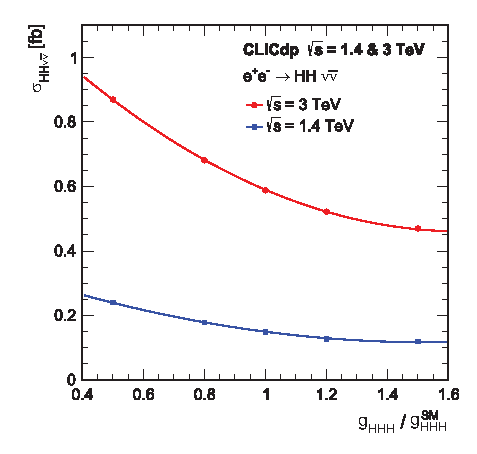
\includegraphics[width=0.45\textwidth]{{doubleHiggs/extraction/oneDrelation2}}
\caption[Cross section for the \eeToHH process as a function of the ratio $\lambda/\lambda_{SM}$ ]
{Cross sections of \eeToHH process as a function of the ratio $\gHHH/\gHHHSM$ at \rootS{1.4} and 3\,TeV, adapted from \cite{Abramowicz:2016zbo}.}
   \label{fig:doubleHiggsCouplingOneDRelation}
\end{figure}
%Without electron polarisation,
The uncertainties on measurement of the Higgs trilinear self coupling, \gHHH, from  \eeToHH $\to$ \HepProcess{ \Pbottom \APbottom \PWplus \PWminus \Pnue \APnue} analyses, are hence obtained via \Equation{eqn:doubleHiggs1Dextration}:
\begin{equation}
\frac{\Delta\gHHH}{\gHHH} \approx
\begin{cases}
  218\%, & \mbox{at \rootS{1.4}, }  \\
  135\%, & \mbox{at \rootS{3}}.
\end{cases}
\end{equation}

Since the leading-order  Feynman diagrams for the double Higgs boson production  include a t-channel $\HepProcess{\PW\PW}$-fusion process, the cross section of the double Higgs production can be enhanced by using a polarised electron beam. For a electron beam polarisation of $P(\Pem) = 80\%$, the uncertainties of the coupling \gHHH  become:
\begin{equation}
\frac{\Delta\gHHH}{\gHHH} \approx
\begin{cases}
  163\%, & \mbox{at \rootS{1.4}, }  \\
  97\%, & \mbox{at \rootS{3}}.
\end{cases}
\end{equation}
When the analyses at both \rootS{1.4} and \rootS{3} are combined, the uncertainty of the coupling \gHHH improves to 99\% with the unpolarised beam, and to 87\% with the polarised beam of  $P(\Pem) = 80\%$.


%\section{Combined results}

When the analyses for \eeToHHbbWW and \eeToHHbbbb sub-channels are combined, the expected uncertainties on the double Higgs production cross section measurements are:
\begin{equation}
\frac{\Delta\left[\sigma\left(\HHvv\right)\right]}{\sigma\left(\HHvv\right)} =
\begin{cases}
  44\%, & \mbox{at \rootS{1.4}, }  \\
  20\%, & \mbox{at \rootS{3}},
\end{cases}
\end{equation}

This translates to uncertainties on the measurement of the Higgs trilinear self coupling \gHHH, via \Equation{eqn:doubleHiggs1Dextration}, with unpolarised beams:
\begin{equation}
\frac{\Delta\gHHH}{\gHHH} \approx
\begin{cases}
  54\%, & \mbox{at \rootS{1.4}, }  \\
  29\%, & \mbox{at \rootS{3}}.
\end{cases}
\end{equation}

\section{Simultaneous couplings extraction}

%As stated in the beginning of the chapter,
%Therefore, a simultaneous extraction on the coupling uncertainty can be performed by extending the one-dimensional coupling extraction in the previous sections.
The study of the double Higgs production via \WW fusion can probe the Higgs trilinear self coupling, \gHHH, and quartic coupling, \gWWHH.  A two-dimensional \gHHH and \gWWHH couplings extraction is performed using the results of the hadronic  analysis at  \rootS{3}. The integrated luminosity in this section is assumed to be 3000\,\uprightMath{fb^{-1}} at  \rootS{3}  to reflect the updated \CLIC running scenario \cite{CLIC:2016zwp}. A simple scaling is applied to the number of events after the MVA event selection for the analysis at \rootS{3} to adapt to  the change in the luminosity.

% , as the uncertainty in couplings obtained from analysis at \rootS{1.4} is too large to obtain meaningful results.
%  template fitting





The \eeToHH events with non-SM \gHHH and \gWWHH  couplings were generated and reconstructed in the same way as previously.  The normalised cross sections of the \eeToHH as a function of \gHHH and \gWWHH are shown in \Figure{fig:doubleHiggsCouplingCrossSection}.  Around the SM coupling values, the cross section increases with the decrease of \gHHH and with the increase of \gWWHH.

%The cross sections along the anti-diagonal are nearly constant, which would be difficult to precisely determine the statistical uncertainty on the coupling measurements.

\begin{figure}[!htbp]
    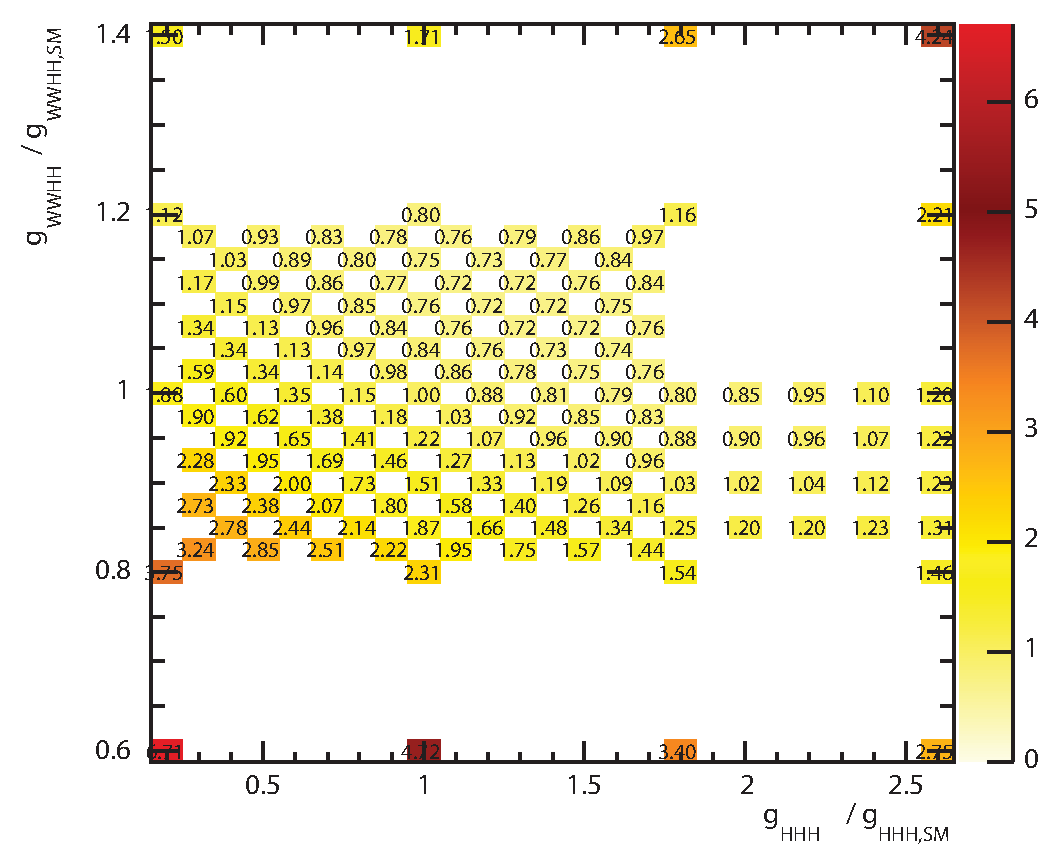
\includegraphics[width=0.85\textwidth]{{doubleHiggs/extraction/crossSectionNew3}}
\caption{Normalised cross section for the \eeToHH process as a function of the $\gHHH/\gHHHSM$ and  $\gWWHH/\gWWHHSM$ at \rootS{3}. All cross sections are normalised to the cross section at the SM couplings value.}
   \label{fig:doubleHiggsCouplingCrossSection}
\end{figure}



%Once a relationship between the couplings, \gHHH and \gWWHH, and the change in kinematic variable distributions is established,  the uncertainty of the measurements of  \gHHH and \gWWHH  be obtained.

%To determine the uncertainty on the coupling measurements, the variables proposed in the  study in \Section{sec:theoryHiggsBSM} are used: the invariant mass of the two Higgs system, \mhh, and the scalar sum of the two Higgs transverse momentum, \HT.  %By choosing kinematic bins, high-energy behaviour can be disentailed from the physics at threshold, allowing the extraction of the coupling strength \gWWHH and \gHHH.
%generator-leve

These generated non-SM coupling \eeToHH events went through the analysis chain described in this chapter with the same pre-selection cuts and the same MVA classifier applied. The same of background events from the \rootS{3} analysis were added to the \eeToHH events with non-SM couplings. \FIGURE{fig:doubleHiggsCouplingSignificancebbWW} shows the  signal significance after the MVA event selection of the double Higgs events with hadronic \WW decay of \eeToHHbbWW sub-channel as a function of  \gHHH and \gWWHH.

\begin{figure}[!htbp]
    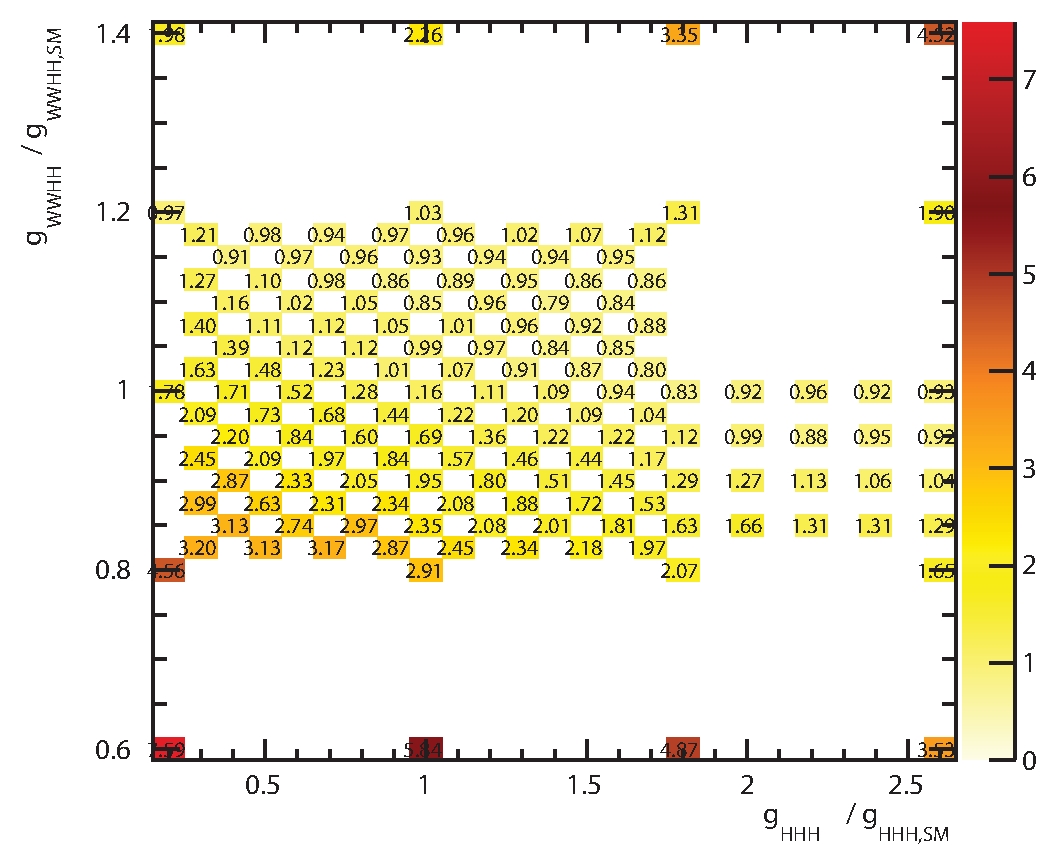
\includegraphics[width=0.8\textwidth]{doubleHiggs/extraction/SignificanceBono4}
\caption{The significance for the \eeToHH process as a function of the $\gHHH/\gHHHSM$ and  $\gWWHH/\gWWHHSM$ at \rootS{3}, using  hadronic \WW decay of \eeToHHbbWW sub-channel, assuming an integrated luminosity of  3000\,\uprightMath{fb^{-1}}.}
   \label{fig:doubleHiggsCouplingSignificancebbWW}
\end{figure}


Two kinematic variables that are sensitive to the change of the couplings, motivated in \Section{sec:theoryHiggsBSM}, are used for the extraction of the couplings: the invariant mass of the two Higgs system, \mhh, and the scalar sum of the two Higgs transverse momentum, \HT.

Events are subsequently binned using the kinematic variables. Two bins in \HT are obtained by dividing the \HT distribution at 200\,GeV. Four bins in \mhh are obtained by dividing the \mhh distribution at 400, 560, and 720\,GeV. This results in events being divided into eight kinematic bins.

%Once the relationship between the change in the kinematic variable distributions, and the change in couplings is established,  the uncertainties of the measurements of  \gHHH and \gWWHH  can be obtained.

%The selected events are divided into 8 kinematic bin. Two bins in \HT are obtained by binning the \HT distribution at 200\,GeV. Four bins in \mhh are obtained by dividing the \mhh distribution at 400, 560, and 720\,GeV.
To access the change in the \mhh and \HT distributions for  non-SM coupling samples, the $\chi^2$ function is used:
%A $\chi^2$ function is constructed to access the change in the \mhh and \HT distributions for  non-SM coupling comparing to \SM coupling sample, defined as:
\begin{equation}
\chi^2 = \sum_{i}^{8}\frac{\parenths{N_i^e - N_{i}^{o}}^2}{N_{i}^e},
\label{eqn:doubleHiggsChi2}
\end{equation}
where $N_i^e$ is the number of expected  events in the kinematic bin $i$ in a non-SM coupling sample; and $ N_{i}^{o}$ is the number of observed  event in the kinematic bin $i$. Here the observed sample is assumed to be the \SM coupling sample. The  $\chi^2$  is summed over all kinematic bins. By construction, the \SM coupling sample has a $\chi^2$ of 0. \FIGURE{fig:doubleHiggsCouplingChi2Separate} shows the $\chi^2$  as a function of \gHHH and \gWWHH using samples from two sub-channels: hadronic \WW decay of \eeToHHbbWW and \eeToHHbbbb. The $\chi^2$ values for the \eeToHHbbbb sub-channel are larger because the signal significance of \eeToHHbbbb  sub-channel is much higher than that of the hadronic \WW decay of \eeToHHbbWW channel.

%more sensitive to the couplings.


\begin{figure}[!htbp]
  \begin{subfigure}[b]{0.75\textwidth}
    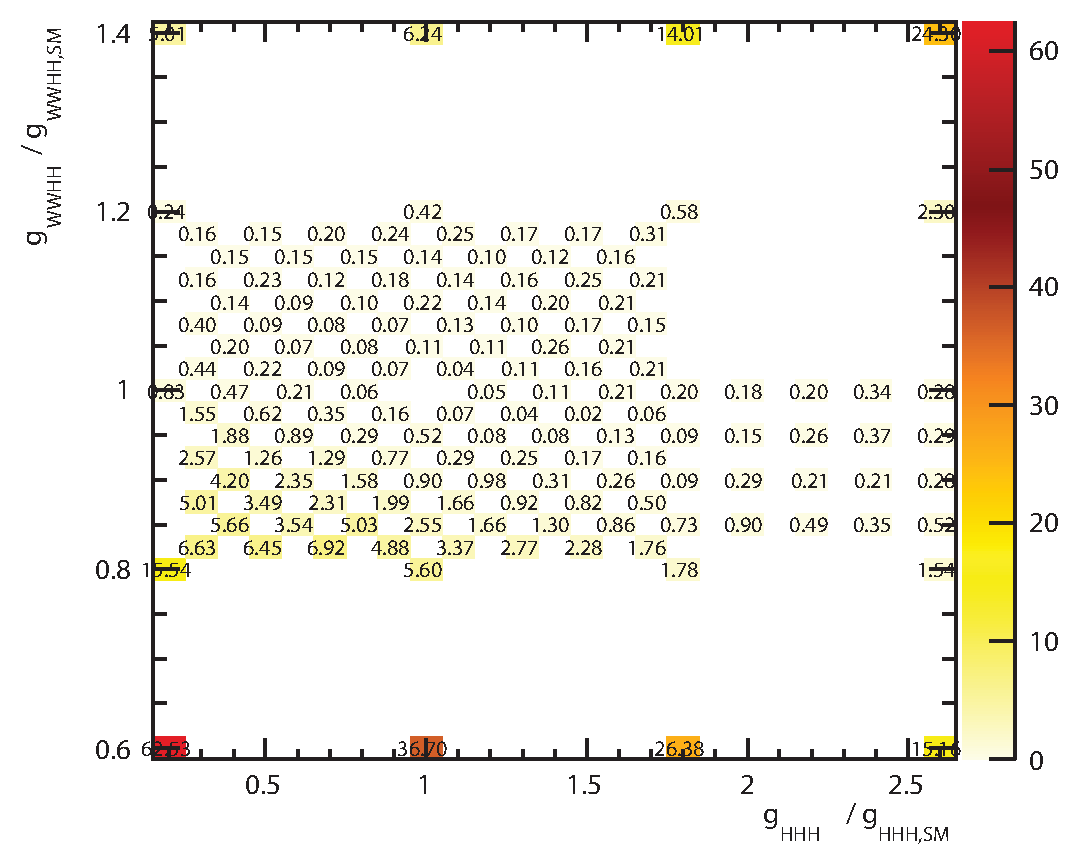
\includegraphics[width=\textwidth]{{doubleHiggs/extraction/new/chi2Bono4mhh2HT3}}
    \caption{\eeToHHbbWWHad}
    \label{fig:doubleHiggsCouplingChi2bbWW}
  \end{subfigure}
    \begin{subfigure}[b]{0.75\textwidth}
    \includegraphics[width=\textwidth]{doubleHiggs/extraction/new/chi2Rosa4mhh2HT3}
    \caption{\eeToHHbbbb}
    \label{fig:doubleHiggsCouplingChi2bbbb}
  \end{subfigure}
\caption[$\chi^2$ as a function of $\gHHH/\gHHHSM$ and  $\gWWHH/\gWWHHSM$  at \rootS{3}]%
   {The $\chi^2$ for the \eeToHH process as a function of the $\gHHH/\gHHHSM$ and  $\gWWHH/\gWWHHSM$ at \rootS{3}, using: a) hadronic \WW decay of \eeToHHbbWW; b) and \eeToHHbbbb sub-channels, assuming an integrated luminosity of  3000\,\uprightMath{fb^{-1}}.}
   \label{fig:doubleHiggsCouplingChi2Separate}
\end{figure}

Two sub-channels, hadronic \WW decay of \eeToHHbbWW and \eeToHHbbbb, are combined to increase the statistical precision on the coupling measurements.  To minimise the statistical fluctuations when generating  samples with different non-SM couplings, a toy MC experiment is performed. The SM coupling sample is treated as a data template set. 100000 data sets are generated by fluctuating the event number in each kinematic bin in the data template according to the Poisson distribution with a mean that is equal to the event number in the bin.  The $\chi^2$ is calculated using these generated data sets as the observed data ($N_{i}^e$ in \Equation{eqn:doubleHiggsChi2}). The $\chi^2$ is then averaged over the number of  data sets (100000) and normalised such that the $\chi^2$ at the  SM couplings is 0. \FIGURE{fig:doubleHiggsCouplingChi2Ave} shows the normalised $\chi^2$ after averaging over 100000 toy MC experiments as a function of $\gHHH/\gHHHSM$ and $\gWWHH/\gWWHHSM$.

%Since only the difference of $\chi^2$  between samples with non-SM couplings and SM couplings  is used for the couplings extraction, this normalisation does not affect the couplings extraction and helps to ease the visualisation.
%The $\chi^2$ changes slowly along the anti-diagonal which is similar to the cross section plot.

\begin{figure}[!htbp]
    \includegraphics[width=0.85\textwidth]{{doubleHiggs/extraction/new/chi2CombineAve4mhh2HT3}}
\caption{Normalised $\chi^2$, after averaging over 100000 toy MC experiments, as a function of $\gHHH/\gHHHSM$ and  $\gWWHH/\gWWHHSM$, after combining hadronic decay \eeToHHbbWW and \eeToHHbbbb sub-channels, assuming an integrated luminosity of  3000\,\uprightMath{fb^{-1}}.  Normalisation is set such that the $\chi^2$ at the  SM coupling point is 0.}
   \label{fig:doubleHiggsCouplingChi2Ave}
\end{figure}


%for this fit
Since there are two couplings in this $\chi^2$ surface, the degree of freedom  is 2. A contour of 68\% confidence ($\chi^2 = 2.3$) can be drawn by interpolating between points on the $\chi^2$ surface in \Figure{fig:doubleHiggsCouplingChi2Ave}. \FIGURE{fig:doubleHiggsCouplingChi2Countour} shows the contour of 68\% confidence of the measurements of the \gHHH and \gWWHH. The counter can be sliced one dimensionally to extract the uncertainty of the measurements of one coupling for a given value of the other coupling. For example:
\begin{equation}
\frac{\Delta\gWWHH}{\gWWHH}  \simeq 4.9\% , & \text{ for \gHHH = $\gHHHSM$},\\
\frac{\Delta\gHHH}{\gHHH}  \simeq 29\% , & \text{ for \gWWHH = $\gWWHHSM$}.
\end{equation}
The statistical precisions on the measurements of \gWWHH and \gHHH are much better at \CLIC than at current \LHC or  high-luminosity upgraded \LHC \cite{Contino:2010mh}.


\begin{figure}[!htbp]
    \includegraphics[width=0.85\textwidth]{doubleHiggs/extraction/new/contourCOmbineAve5}
\caption{Contour plot of 68\% confidence ($\chi^2 = 2.3$) , after averaging toy MC experiments, as a function of $\gHHH/\gHHHSM$ and  $\gWWHH/\gWWHHSM$,  after combining hadronic \WW  decay of \eeToHHbbWW and \eeToHHbbbb sub-channels, assuming an integrated luminosity of  3000\,\uprightMath{fb^{-1}}.}
   \label{fig:doubleHiggsCouplingChi2Countour}
\end{figure} 